% !TEX TS-program = pdflatex
% !TEX encoding = UTF-8 Unicode
\RequirePackage{fix-cm}
\documentclass[ngerman,a4paper,openany,showtrims]{memoir}
% !TEX ROOT = ersti.tex
\usepackage{fixltx2e}

\usepackage[ngerman]{babel}
\usepackage{color}

\usepackage[utf8]{inputenc} % wir wollen das erstiinfo /richtig/
                            % kodiert haben

% Boolean, mit dem wir abfragen können, ob Druck- oder Webversion benötigt wird,
% um nicht alles in config_druck.tex bzw. config_web.tex angeben zu müssen.
\usepackage{ifthen}
\newboolean{druckversion}

% Diese Datei wird automatisch vom Makefile erstellt aus config_web.tex
% und config_druck.tex, je nachdem was man will
\input{config.tex}

\usepackage{eurosym} % eurozeichen kann man schon gut gebrauchen
\usepackage{amsmath}

\usepackage{memhfixc} % fix für die kollision memoir/hyperref

\usepackage{euler} % euler ist die schrift für die kapitelüberschriften
\usepackage{wasysym}  % für die Simleys
\usepackage[squaren]{SIunits}  % für "m^2" und andere Maßeinheiten
\usepackage{newcent}
\usepackage[pdftex]{graphicx} % hübsche bilder
\usepackage{epstopdf} % direkt eps einbinden können
\usepackage{booktabs} % hübsche tabellen
\usepackage[protrusion=true,expansion]{microtype} % hübscherer Blocksatz
\usepackage{multirow} % mehrzeilige Spalten in Tabellen
\usepackage[T1]{fontenc}

\usepackage{timetable} % für die Stundenpläne
\defineeventgrey{xxxxxx}{1.00}{0.0}
\defineeventgrey{xxxxx} {0.96}{0.0}
\defineeventgrey{xxxx}  {0.86}{0.0}
\defineeventgrey{xxx}   {0.76}{0.0}
\defineeventgrey{xx}    {0.66}{0.0}
\defineeventgrey{x}     {0.56}{0.0}

\usepackage[section=chapter,numberline,nonumberlist]{glossaries}
\renewcommand*{\glsclearpage}{\clearpage}
\makeglossaries
% Kurzanleitung:
% http://mirror.ctan.org/macros/latex/contrib/glossaries/glossariesbegin.pdf

% Syntax:
% \newglossaryentry{ label }{ settings }
% \newacronym{ label }{ abbrv }{ full }


% Beispiele: Einträge erstellen
% \newglossaryentry{electrolyte}{name=electrolyte, description={solution able to conduct electric current}}

% \newglossaryentry{oesophagus}{name=œsophagus, description={canal from mouth to stomach}, plural=œsophagi}

% \newacronym{label}{svm}{support vector machine}


% Beispiel: sich auf einen Glossareintrag beziehen
%       \gls{ label }
%       \glspl{ label }   % gibt die Pluralform aus


\newglossaryentry{c.t.}{name={c.t.}, description={lat.: cum tempore, mit Zeit. Also eine viertel Stunde später}}
\newglossaryentry{s.t.}{name={s.t.}, description={lat.: sine tempore, ohne Zeit. Also genau so, wie es da steht}}
\newglossaryentry{HEIDI}{name={HEIDI}, description={So heißt das Computersystem der \gls{UB}, mit dem ihr nach Büchern suchen und sie auch gleich vorbestellen könnt. Eure aktuellen Ausleihen werden auch dort gelistet, ebenso besteht die Möglichkeit dort insgesamt zweimal eure Ausleihfristen um je einen Monat zu verlängern. Die Adresse ist \url{http://heidi.ub.uni-heidelberg.de}, aber eine Suche nach „heidi heidelberg“ führt auch zum Ziel}}


\newglossaryentry{URZ}{
	name={URZ},
	first={Universitätsrechenzentrum (URZ)},
	description={Das Universitätsrechenzentrum stellt alles bereit, was sich grob mit dem Begriff „Computer“ in Verbindung bringen lässt. Siehe Artikel auf \autopageref{urz}}
}

\newglossaryentry{AM}{
	name={AM},
	first={Angewandte Mathematik (AM, INF 294)},
	description={In der Angewandten Mathematik befinden sich die Bereichsbibliothek sowie ein Kopierer, an dem Mathe- und Infostudis aus Studiengebühren finanziert kopieren können. Die Kopierkarte kann bei der Bibliotheksaufsicht gegen Studi- und Personalausweis ausgeliehen werden. Unseres Wissens nach ist dies auch das einzige Gebäude mit negativen Raumnummern. Wenn ihr also eine Übungsgruppe in „-104“ habt, ist der Keller der AM gemeint}
}

\newglossaryentry{RM}{
	name={RM},
	first={Reine Mathematik (RM, INF 288)},
	description={Die Reine Mathematik ist das Gebäude INF 288. Im ersten Stock befinden sich die Prüfungssekretariate der Mathe}
}

\newglossaryentry{GymPO}{
	name={GymPO I},
	first={Gymnasiallehrerprüfungsordnung I (GymPO I)},
	description={Die „Gymnasiallehrerprüfungsordnung I“ ist die Prüfungsordnung, nach der sich alle Lehrämtler\_innen ab dem WS 2010/2011 prüfen lassen müssen. Siehe Artikel auf \autopageref{lehramt_allg}}
}

\newglossaryentry{EPG}{
	name={EPG},
	first={Ethisch-Philosophische Grundlagenstudium (EPG)},
	description={Das Ethisch-Philosophische Grundlagenstudium ist ein Teil des Lehramtsstudiums. Siehe Artikel auf \autopageref{epg}}
}
\newglossaryentry{OMZ}{
    name={OMZ},
    first={Otto-Meyerhof-Zentrum (OMZ)},
    description={Im OMZ findet ihr das Robotiklabor, ein paar Seminarräume und einen großen CIP-Pool, in dem z.B. der Programmierkurs stattfindet}
}

\newglossaryentry{FSK}{
	name={FSK},
	first={Fachschaftskonferenz (FSK)},
	description={Die Fachschaftskonferenz war der vorgänger des StuRa als Vertretung aller Studis vor der Wiedereinführung der Verfassten Studierendenschaft}
}

\newglossaryentry{StuRa}{
	name={StuRa},
	first={Studierendenrat (StuRa)},
	description={Der StuRa ist das Zentralorgan der Verfassten Studierendenschaft an der Uni Heidelberg und tagt zweiwöchentlich im neuen Hörsaal am Philosophenweg. Details in den Artikeln auf \autopageref{hopo} ff}
}

\newglossaryentry{ZFB}{
	name={ZFB},
	first={Zentrales Fachschaftenbüro (ZFB)},
	description={auch: StuRa-Kontor. Büro- und Tagungsräume für den StuRa und andere studentische Gruppen. Auch die Sozialberatung u.ä. finden hier statt. Die genaue Adresse ist Albert-Ueberle-Straße 3-5, 69120 Heidelberg}
}


\newglossaryentry{KVV}{
	name={KVV},
	first={Kommentiertes Vorlesungsverzeichnis (KVV)},
	description={Das Kommentiertes Vorlesungsverzeichnis enthält eine Beschreibung zu vielen Veranstaltungen, die neben „Wer? Wo? Wann?“ auch Auskunft über den Inhalt gibt. Literaturempfehlungen und Voraussetzungen können hier ebenfalls nachgelesen werden.\\ \url{http://www.ub.uni-heidelberg.de/helios/fachinfo/www/math/kvv/}}
}


\newacronym{UB}{UB}{Universitätsbibliothek}
\newacronym{OPNV}{ÖPNV}{Öffentlicher Personen Nahverkehr}
\newacronym{INF}{INF}{im Neuenheimer Feld}
\newacronym{HS}{HS}{Hörsaal}
\newglossaryentry{FSWE}{
	name={FSWE},
	first={Fachschaftswochenende (FSWE)},
	description={Das Fachschaftswochenende veranstalten wir einmal pro Semester um Themen diskutieren können, die sich nicht sinnvoll in einer Fachschaftssitzung unterbringen lassen. Und jede Menge Spaß haben natürlich \smiley. Die Mitfahrt ist für euch kostenlos.}
}

\newglossaryentry{SWS}{
	name={SWS},
	first={Semesterwochenstunden (SWS)},
	description={Die Semesterwochenstunden geben an, wie viel Aufwand eine Veranstaltung ungefähr ist. Genau genommen wird nur die Anwesenheitszeit pro Woche angegeben: Ein Seminar hat dann meist 2 SWS, eine Vorlesung mit Übung dagegen 4+2 SWS}
}



\newacronym{ZUV}{ZUV}{Zentrale Universitätsverwaltung}
\newacronym{StuWe}{StuWe}{\href{www.studentenwerk.uni-heidelberg.de}{Studentenwerk}}

% Für bestimmte Akronyme, die keine Mehrzahl haben, missbrauchen wir das
% Mehrzahlfeld um Genitiv (oder so… "des KIPs") zu speichern
\newacronym[\glslongpluralkey={Kirchoff-Instituts für Physik},\glsshortpluralkey={KIP}]{KIP}{KIP}{Kirchoff-Institut für Physik}
\newglossaryentry{PI}{
	name={PI},
	first={Physikalisches Institut (PI)},
	description={Das PI wird des öfteren auch Klaus-Tschira-Institut genannt. Es handelt sich dabei um eines der neueren Gebäude im Feld. Dort finden eure ersten verpflichtenden Physikpraktika statt, welche aus diversen Versuchen bestehen.}
}
\newacronym[\glslongpluralkey={Verkehrsverbundes Rhein-Neckar},\glsshortpluralkey={VRN}]{VRN}{VRN}{Verkehrsverbund Rhein-Neckar}

% Zeige alle Einträge an, auch die ohne Referenz
\glsaddall


% alternative Fußnoten-Symbole
\makeatletter
\newcommand*{\@greek}[1]{\ensuremath{\ifcase#1 \or \alpha \or \beta \or \gamma \or \delta \or \varepsilon \or \zeta \or \eta \or \vartheta \or \iota \or \kappa \or \lambda \or \mu \or \nu \or o \or \pi \or \varrho \or \sigma \or \tau \or \upsilon \or \varphi \or \chi \or \psi \or \omega \or \varsigma \else \@cterr \fi}}
\newcommand*{\greek}[1]{\expandafter\@greek\csname c@#1\endcsname}
\makeatother
\renewcommand{\thefootnote}{\greek{footnote}}

% !TEX ROOT = ../ersti.tex
% hier werden die Posten definiert, damit bei Neuwahlen nicht der
% Text durchsucht werden muss

% BITTE BEACHTEN:
%  - Titel sind Böse. Keine Titel. Keine Titel.
%  - Keine abschließenden Leerzeichen. Das ist einfach falsch und flahsc.

%Physik
\newcommand{\dekanphysik}{Hebecker}
\newcommand{\dekanphysiklang}{Arthur Hebecker}
\newcommand{\dekanphysikfoto}{bilder/hebecker_mon.jpg}
\newcommand{\prodekanphysik}{Hans-Christian Schulz-Coulon und Matthias Weidemüller}
\newcommand{\prodekanphysikA}{H.-C. Schulz-Coulon}
\newcommand{\prodekanphysikfotoA}{bilder/hcsc_mon.jpg}
\newcommand{\prodekanphysikB}{M. Weidemüller}
\newcommand{\prodekanphysikfotoB}{bilder/weidemueller_mon.jpg}
\newcommand{\studiendekanphysik}{Norbert Herrmann}
\newcommand{\studiendekanphysikfoto}{bilder/herrmann_mon.jpg}
\newcommand{\pruefausschussvorsitzphysik}{Cornelis Dullemond}
\newcommand{\studienberatungphysik}{Ulrich Uwer und Michael Hausmann}
\newcommand{\dozentvorkurs}{Herrn Thommes und Herrn Komnick}
\newcommand{\bafogphysik}{Norbert Herrmann}
\newcommand{\dekanatphysik}{Dewald-Klussmann}
\newcommand{\dekanatphysiktelefon}{+49\,62\,21 / 54\,-\,92\,98}
\newcommand{\frauenbeauftragtephysik}{Monica Dunford}
\newcommand{\pruefsekphysik}{Frau Hiemenz und Frau Nerger}
\newcommand{\pruefsekphysikfotoA}{bilder/hiemenz_mon.jpg}
\newcommand{\pruefsekphysikA}{Frau Hiemenz}
\newcommand{\pruefsekphysikfotoB}{bilder/nerger_mon.jpg}
\newcommand{\pruefsekphysikB}{Frau Nerger}


%Mathe
\newcommand{\dekanmathe}{Gertz}
\newcommand{\dekanmathelang}{Michael Gertz}
\newcommand{\dekanmathefoto}{bilder/gertz_mon.jpg}
\newcommand{\prodekanmathe}{Kay Wingberg}
\newcommand{\prodekanmathefoto}{bilder/wingberg_mon.jpg}
\newcommand{\studiendekanmathe}{Guido Kanschat}
\newcommand{\studiendekanmathefoto}{bilder/kanschat_mon.jpg}
\newcommand{\pruefausschussvorsitzmathe}{Gebhard Böckle}
\newcommand{\studienberatungmathe}{Karl Oelschläger und Winfried Kohnen}
\newcommand{\frauenbeauftragtemathe}{Anna Marciniak-Czochra}
\newcommand{\bafogmathe}{Markus Banagl}
\newcommand{\dekanatmathe}{Frau Häukäufer}
\newcommand{\dekanatmathetelefon}{+49\,62\,21 / 54\,-\,57\,58}
\newcommand{\pruefsekmathe}{Frau Kiesel}
\newcommand{\pruefsekmathefoto}{bilder/kiesel_mon.jpg}

%Info
\newcommand{\studiendekaninformatik}{Artur Andrzejak}
\newcommand{\studiendekaninformatikfoto}{bilder/andrzejak_mon.jpg}
\newcommand{\studienberatunginformatik}{Wolfgang Merkle}
\newcommand{\pruefausschussvorsitzinformatik}{Gerhard Reinelt}
\newcommand{\bafoginformatik}{Peter Bastian}
\newcommand{\pruefsekinfo}{Frau Sopka}
\newcommand{\pruefsekinfofoto}{bilder/sopka_mon.jpg}

%Uni
\newcommand{\frauenbeauftragteuni}{Jadranka Gvozdanovic}
\newcommand{\rektor}{Bernhard Eitel}
\newcommand{\fskstudisimsenat}{keinen der vier}

%Rest
\newcommand{\redaktionsschluss}{08.08.2015}
\newcommand{\volley}{im Dezember}                 % "Der nächste Termin ist ...   ."
\newcommand{\anfi}{9.\,Oktober 2015}               % Termin für die AnfiFete
\newcommand{\fsraum}{\Gls{INF} 305, Raum 045}
\newcommand{\auflage}{850}                        % wie viel Erstiinfos sollen
                                                  % gedruckt werden
\newcommand{\semester}{Wintersemester 2015/16}    % bislang nur fuer titel.tex

% wo fehlt noch
\newcommand{\fswe}{6. bis 8. November} % Dieses Semester findet es am <Datum> statt.

\newcommand{\mathphystheotermin}{17.\,Oktober 2014}

% diverse Minister

\newcommand{\wissenschaftsministerbawue}{Theresia Bauer (Grüne)}
\newcommand{\wissenschaftsministerbund}{Johanna Wanka (CDU)}


% Geldbeträge
%\newcommand{\studiengebuehren}{500}
\newcommand{\verwaltungsbetrag}{60}
\newcommand{\studentenwerksbeitrag}{74,80}
\newcommand{\vsbeitrag}{7,50}
\newcommand{\beitragssumme}{142,30}
\newcommand{\quasimi}{280}

% http://www.vrn.de/vrn/tickets/zeitkarten/studenten/vrn-semesterticket/index.html
\newcommand{\semesterticket}{150}

%%% Local Variables:
%%% mode: latex
%%% TeX-master: "ersti"
%%% End:
 %% hier sind die ganzen wichtigen
                               %% aktualisierungswürdigen daten
                               %% drin. das ist wichtig!!!

%%%%%% eigens definierter krimskrams


\newenvironment{spalten}{}{}
\newcommand{\nurimdruck}[1]{#1}
\newcommand{\email}[1]{\href{mailto:#1}{#1}}
% Dieser Befehl wird genutzt, um die Comics/Bilder am Rand, die auf
% einer „neues Kapitel“-Seite sind nach unten zu verschieben, um
% Überlappungen zu verhindern.
\newcommand{\chaptersidebarpushdown}{\vspace*{6.47cm}}
\setsidebarheight{22cm}

\urlstyle{same}

%%%% chapterstyle

\makechapterstyle{mathphys}{
    \renewcommand{\chaptitlefont}{
        \checkoddpage
        \ifoddpage
            \Huge\flushright\sffamily
        \else
            \Huge\flushleft\sffamily
        \fi
    }
    \renewcommand{\printchaptertitle}[1]{
        \checkoddpage
        \ifoddpage
            % gerade seiten
            \colorbox{kapitelhintergrund}{
                \parbox{18cm}{
                    \vspace{0.5cm}
                    \parbox{0.985\textwidth}{
                        \chaptitlefont ##1
                    }
                    \hspace*{2.3cm}%
                    \raisebox{-9mm}{
                        \makebox[0pt][l]{
                            \resizebox{!}{42pt}{\chapnumfont
                            % das ist nicht nett. stimmt. tut mir leid. ehrlich.
                            \textcolor{white}{$\thechapter$}}
                        }
                    }
                    \vspace{0.6cm}
                }
            }
        \else
            % ungerade seiten
            \hspace*{-\foremargin}
            \hspace*{-11.2mm} % keine Ahnung warum die fehlen
            \colorbox{kapitelhintergrund}{
                \parbox{18cm}{
                    \vspace{0.5cm}
                    \hspace{1.42cm}
                    \raisebox{-9mm}{
                        \makebox[0pt][l]{
                            \resizebox{!}{42pt}{\chapnumfont
                            \textcolor{white}{$\thechapter$}}
                        }
                    }
                    \hspace*{3.4cm}%
                    \parbox{0.985\textwidth}{
                        \chaptitlefont ##1
                    }
                    % keine Ahnung warum die \colorbox sonst höher wird
                    \vspace{0.56cm}
                }
            }
        \fi
    }

    \renewcommand{\chapnumfont}{\sffamily\bfseries}
    \renewcommand{\printchaptername}{}
    \renewcommand{\afterchapternum}{}
    \renewcommand{\printchapternum}{}
    \renewcommand{\printchapternonum}{}
}


\chapterstyle{mathphys}

\newcommand{\mathphyssubsubsec}[1]{\noindent\sffamily\bfseries\flushleft\textcolor{sectiontextfarbe}{#1}}
\newcommand{\mathphyssubsec}[1]{\large\mathphyssubsubsec{#1}}
\newcommand{\mathphyssec}[1]{
    % Die Trennlinie nach neuen Kapiteln nicht zeichnen
	\ifthenelse{\value{section}>1}{
			\noindent\vspace{-0.2cm}\hrulefill\vspace{0.3cm}
		}{}
%    \ifnum \value{section}=1 \else
%        \noindent\vspace{-0.2cm}\hrulefill\vspace{0.3cm}
%    \fi
    \Large\mathphyssubsubsec{#1}
}
\setsecheadstyle{\mathphyssec}
\setsubsecheadstyle{\mathphyssubsec}
\setsubsubsecheadstyle{\mathphyssubsubsec}
\setparaheadstyle{\sffamily\textbf}
\setsecnumformat{}

\newcommand{\mathphyssecnobar}[1]{
    \begingroup
        \Large\mathphyssubsubsec{#1}\\[1em]
        \addcontentsline{toc}{section}{\numberline{\thesection}#1}
    \endgroup\noindent
}


%\renewcommand{\section}[1]{
%     \addcontentsline{toc}{section}{#1}
                % Wie soll der TOC-Eintrag aussehen?
                % Text ohne Zähler.
%}

\pagestyle{plain}
\makeoddfoot{plain}{}{}{\thepage}
\makeevenfoot{plain}{\thepage}{}{}


%%%% Impressum
\newcommand{\impressum}[2]{
    \vspace*{\fill}
    \begin{tabular*}{0.77\textwidth}{ll}
        \multicolumn{2}{l}{
            \parbox{0.77\textwidth}{
                Der Redaktionsschluss für diesen Text war am #1. Wir freuen uns
                sehr über Kommentare, Anregungen, Verbesserungsvorschläge,
                Mitarbeit und Kuchen -- melde dich bei
				\email{vorkurs@mathphys.fsk.uni-heidelberg.de}.
            }
            \vspace{5cm}
        }\\
        V.\,i.\,S.\,d.\,P.: & Fachschaft MathPhys\\
        & Uni Heidelberg \\
        & Im Neuenheimer Feld 305, Raum 045\\
        & 0\,62\,21 54\,-\,41\,67\\
        & \email{fachschaft@mathphys.fsk.uni-heidelberg.de}\\
        & \url{http://mathphys.fsk.uni-heidelberg.de}\\
    \end{tabular*}

    \vfill

    \begin{textblock*}{202mm}[0,1](8mm,290mm)
        \begin{flushleft}
            \footnotesize\noindent
            ISSN: \ifthenelse{\boolean{druckversion}}{2199-8310}{2199-8329}\\
            Letzter Commit: \input{GITHASH}\\
            Letzte Änderung: \input{GITDATE}\\
			Source Code: \ifthenelse{\boolean{druckversion}}{https://github.com/FachschaftMathPhys/Ersti-Info/tree/\drucktag}{\url{https://github.com/FachschaftMathPhys/Ersti-Info/tree/\webtag}}\\
        \end{flushleft}
    \end{textblock*}

    \begin{textblock*}{203mm}[0,1](-7mm,290mm)
        \begin{flushright}
            \footnotesize
%            \href{http://www.flickr.com/photos/99962592@N00/2849889847/}{Ursprüngliches Coverfoto: Niki Odolphie} \href{http://creativecommons.org/licenses/by/2.0/deed.en}{(CC-BY)}\\ %2009
%            \href{http://www.flickr.com/photos/atoach/6014917153/}{Ursprüngliches Coverfoto: Tim Green} \href{http://creativecommons.org/licenses/by/2.0/deed.en}{(CC-BY)}\\ %2011
%            \href{mailto:mo+erstiinfo@mathphys.fsk.uni-heidelberg.de}{Coverbild: Moritz Brinkmann} \href{http://creativecommons.org/licenses/by-sa/3.0/deed.en}{(CC-BY-SA)}\\ %2012
%            \href{mailto:mo+erstiinfo@mathphys.fsk.uni-heidelberg.de}{Coverbild: Moritz Brinkmann} \href{http://creativecommons.org/licenses/by-sa/3.0/deed.en}{(CC-BY-SA)}\\ %2013
%            \href{http://mo.uni-hd.de/}{Coverbild: Moritz Brinkmann} \href{http://creativecommons.org/licenses/by-sa/4.0/}{(CC-BY-SA)}\\ %2014
            \href{http://mobrinkmann.de}{Coverbild: Moritz Brinkmann} \href{http://creativecommons.org/licenses/by-sa/4.0/}{(CC-BY-SA)}\\ %2015  
            \href{http://xkcd.com/}{xkcd Comics: Randall Munroe} \href{http://creativecommons.org/licenses/by-nc/2.5/}{(CC-BY-NC)}\\
            \href{http://abstrusegoose.com/}{Abstruse Goose Comics: lcfr} \href{http://creativecommons.org/licenses/by-nc/3.0/us/}{(CC-BY-NC)}\\
            \href{http://nfccomic.com/index.php}{Not From Concentrate Comics: \copyright{} Thomas Dobrosielski}\\
            \href{http://www.phdcomics.com/}{Piled Higher and Deeper (PhD) Comics: \copyright{} Jorge Cham}\\
            \href{http://mbah.deviantart.com/art/Evil-Tram-126691939}{Straßenbahn: Henno Lauinger} \href{http://creativecommons.org/licenses/by-nc-sa/3.0/}{(CC-BY-NC-SA)}\\
            \href{http://www.openstreetmap.org/}{Landkarten: Mitarbeiter der OpenStreetMap} \href{http://creativecommons.org/licenses/by-sa/2.0/}{(CC-BY-SA)}
        \end{flushright}
    \end{textblock*}
}

%%%%%%%%% Suche nach Grafiken in ./bilder und .:
\graphicspath{{./bilder/}{./}}

%%%%%%%%% Dschungelbuch Verweise
\newcommand{\dschungel}{
    \marginpar{
        \centering
        \hyperref[dschungel] {
            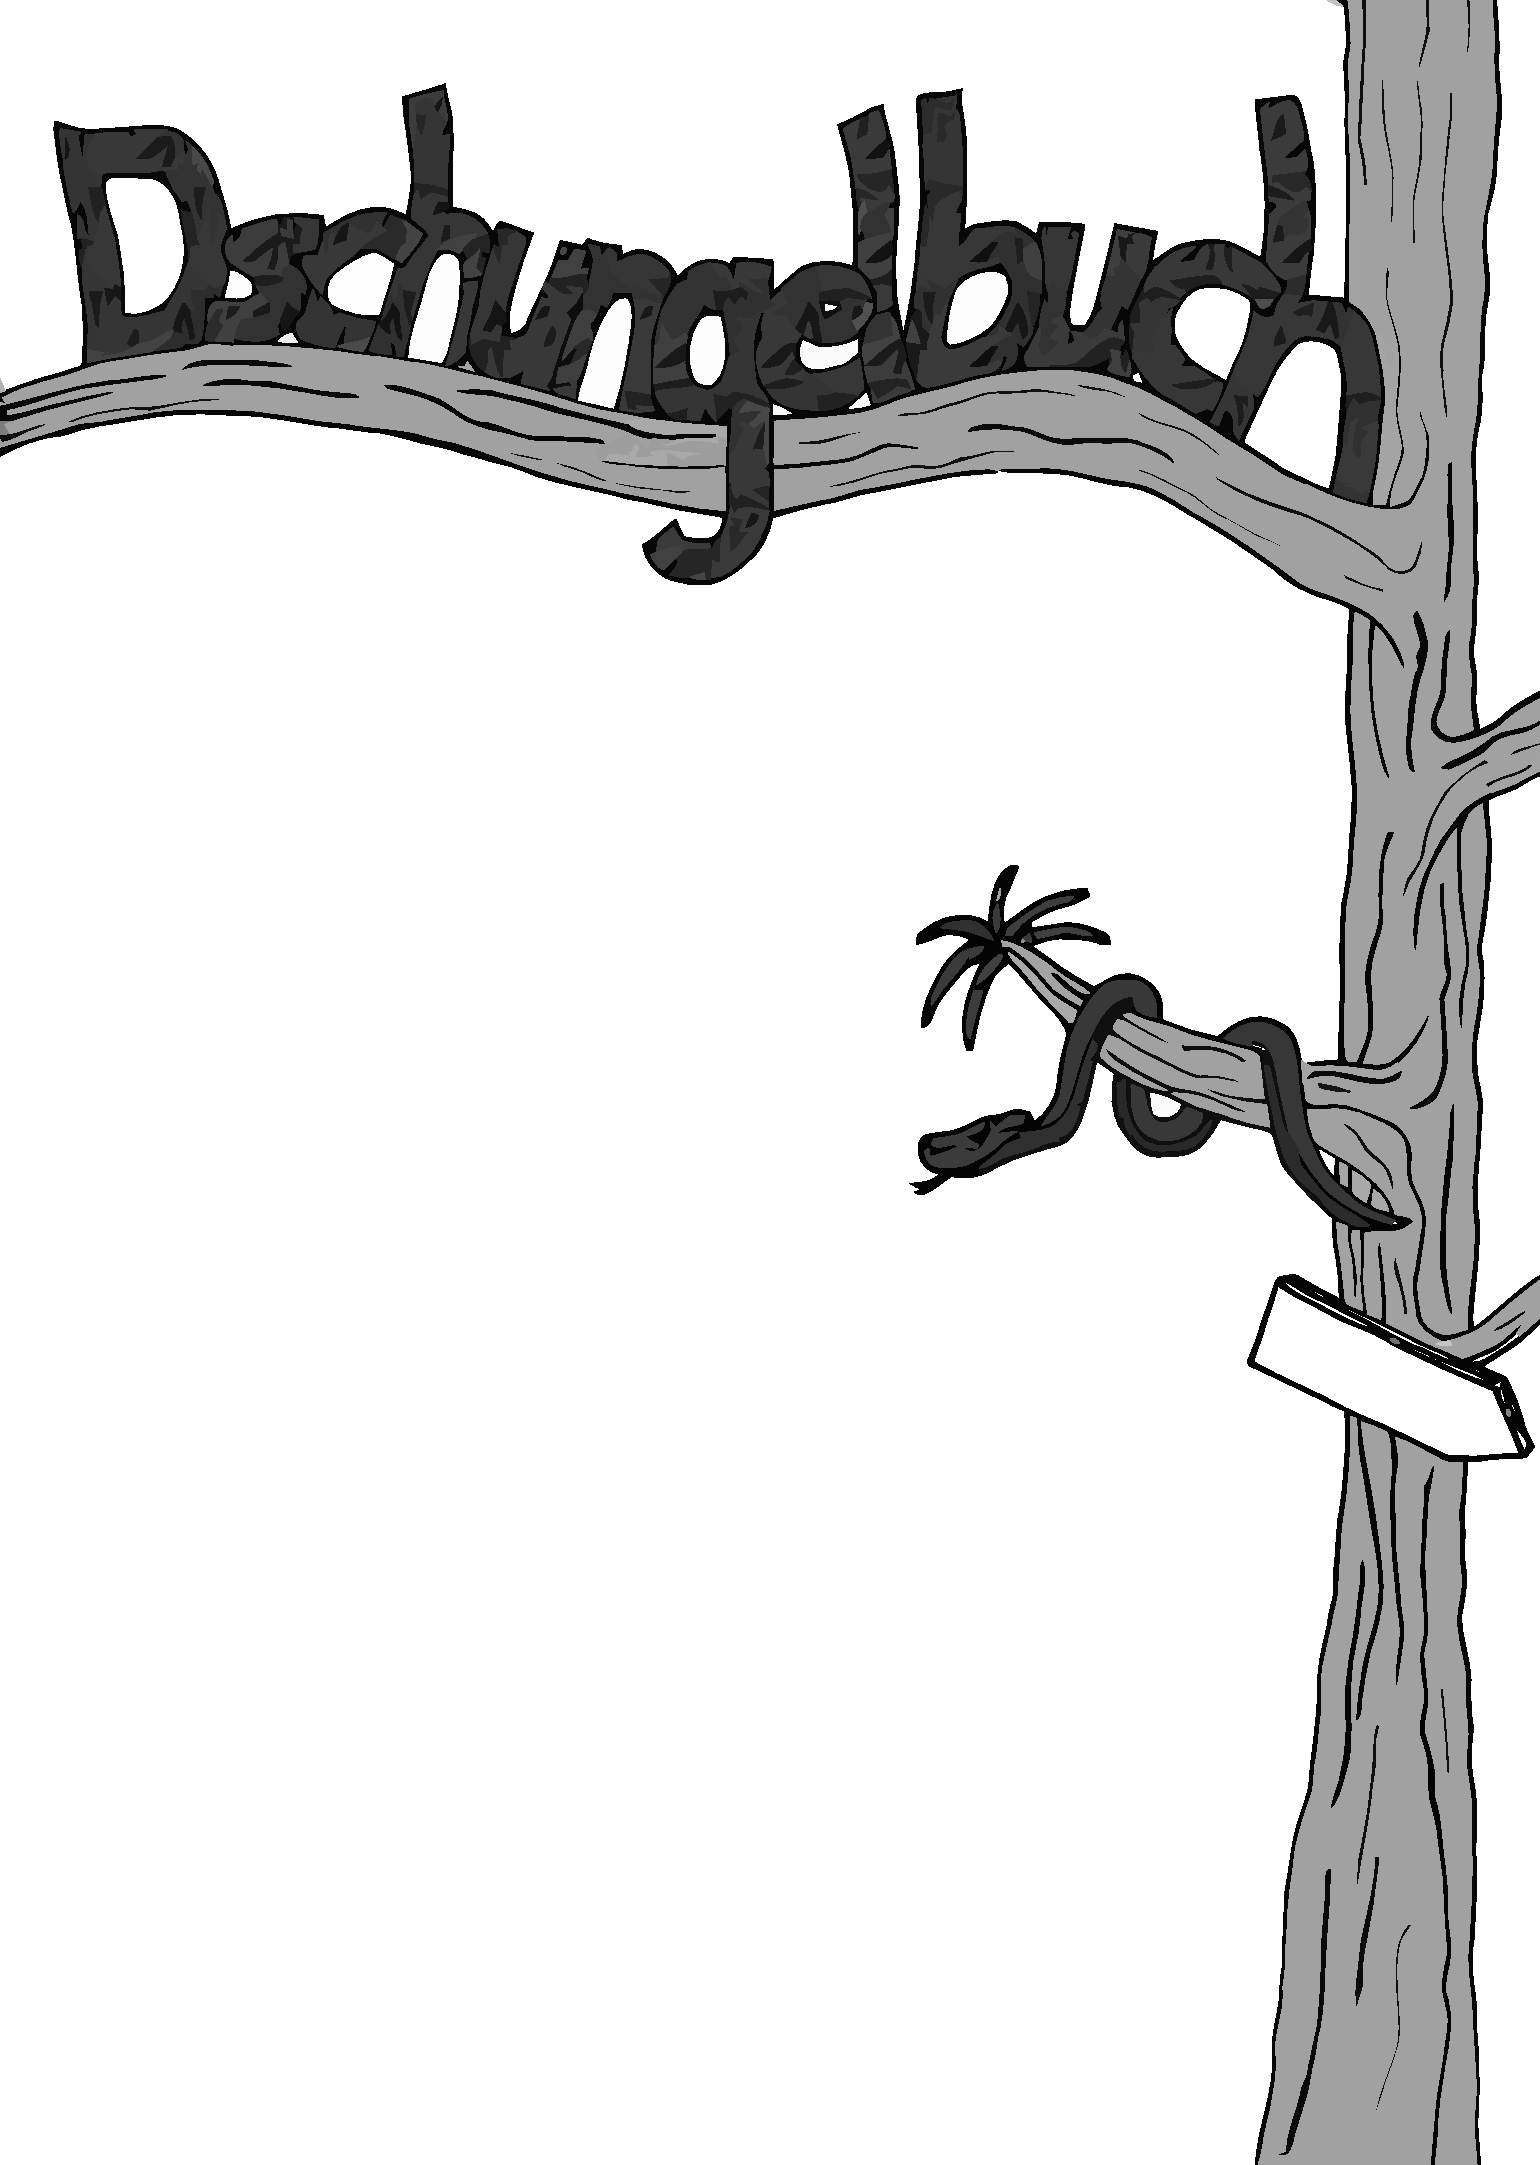
\includegraphics[width=3cm]{dschungelbuch_3.pdf}
        }
    }
}
%%% Local Variables:
%%% mode: latex
%%% TeX-master: ersti
%%% End:


\begin{document}
\pagestyle{empty}

\frontmatter

\tableofcontents

\mainmatter
\pagestyle{plain}

\chapter{Hallo und herzlich willkommen}
 an der Uni Heidelberg! Wenn ihr dieses Erstsemester-Info in den Händen haltet,
 habt ihr euch wahrscheinlich dazu entschieden, hier Informatik, Mathematik
 oder Physik zu studieren -- herzlichen Glückwunsch zu diesem großen und
 wichtigen Schritt! Heidelberg ist eine wunderschöne Stadt und die
 naturwissenschaftlichen Fakultäten der Universität haben national und
 international einen hervorragenden Ruf. Auch das Verhältnis zwischen den
 Professoren und den Studierenden ist in aller Regel überdurchschnittlich gut
 -- einem erfolgreichen, interessanten und lehrreichen Studium steht also
 nichts mehr im Wege. Dabei wünschen wir euch erstmal viel Spaß! \smiley

Da es erfahrungsgemäß vor allem am Anfang des Studiums trotzdem ein
paar Probleme gibt, was die neuen Strukturen an der Uni, den
Studienalltag und so wichtige Nebensächlichkeiten wie Wohnen,
Finanzen, Ausgehen (aber auch Soziales, Umwelt und Politik) gibt, will
die Fachschaft versuchen, euch mit dieser Info-Broschüre einige
nützliche Tipps und Starthilfen für den Uni-Dschungel mit auf den Weg
zu geben \dots

\sidebar{
    \chaptersidebarpushdown
    \centering
    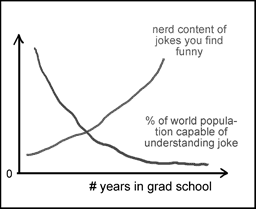
\includegraphics[width=\sidebarwidth]{bilder/Humor.png}\\\vspace{54mm}
    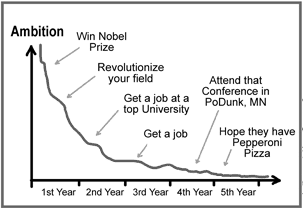
\includegraphics[width=\sidebarwidth]{bilder/ambition.png}
}

Wir hoffen, dass alles Wichtige angesprochen wird. Falls ihr noch
Fragen, Anregungen oder Kritik habt, könnt ihr euch jederzeit an uns
wenden (wo der Fachschaftsraum liegt seht ihr auf der letzten Innenseite).

Falls ihr euch jetzt fragt, wer oder was die Fachschaft eigentlich ist
und was wir außer dem Erstsemester-Info noch alles machen, dann könnt
ihr dies im Kapitel Fachschaft MathPhys nachlesen. \\\\ \noindent Viel Spaß und Erfolg
im Studium,\\\\

eure Fachschaft MathPhys


%%%%%%%%%%%%%%%%%%%%%%%%%%%%%%%%%%%%%%%%%%%%%%%%%%%%%%%%%%%%%%%%%%%%%%%%%%%%%
\chapter{Vorkurs}
% !TEX ROOT = ../ersti.tex
\section{Vorkurs: Informatik}
\label{vkinfo}
Da in den ersten beiden Semestern verhältnismäßig viel Mathe gemacht werden muss, ist der Mathe-Vorkurs auch allen zukünftigen Infostudierenden zu empfehlen. Er widmet sich einer Einführung in die universitäre Mathematik, sowie der Vorstellung einiger anderer Themengebiete. Siehe dazu weiter
\ifthenelse{\pageref{vkmathe} < \pageref{vkinfo}}{oben}{unten}.
Parallel zu den Mathevorträgen zum Thema „Gruppen“ und „Was ist Mathe?“ finden für die InformatikerInnen Informatik-Vorträge statt.

\vskip-5\parskip

\subsection{Programmiervorkurs}
Der Programmiervorkurs richtet sich an alle diejenigen von Euch, die noch keinerlei Kenntnisse im Bereich des Programmierens haben und sich im allgemeinen Umgang mit dem Computer unsicher fühlen. Der Kurs findet vom 21. bis 25. September im OMZ, \gls{INF} 350, statt und ist auch für MathematikerInnen zu empfehlen.

Die Kenntnisse werden in der Einführung in die praktische Informatik (erstes
Semester) bzw. spätestens in Numerik 0 hilfreich sein. Davon abgesehen ist es
nützlich erste Erfahrungen mit unix-artigen Betriebssystemen („Linux“) zu
machen, da sie im naturwissenschaftlichen Bereich weit verbreitet sind.

Für den Programmiervorkurs ist aufgrund der begrenzten Plätze im Computer-Pool
eine vorherige Anmeldung erforderlich!


% !TEX ROOT = ../ersti.tex
\section{Vorkursplan: Mathematik}
\label{vkmathe}
Der Vorkurs für die Studienanfänger der Mathematik und Informatik wird von der
Fachschaft MathPhys organisiert. Er soll helfen, euch den Einstieg in das
Studium zu erleichtern. Dazu gibt es vormittags fachliche Vorträge und Übungen
und nachmittags alles, was nicht direkt mit Mathe zu tun hat: wichtige Infos zu
wechselnden Themen und ein umfangreiches Kennenlern- und Spaßprogramm. Die
Veranstaltungen finden an unterscheidlichen Orten statt, die im Plan rechts
abzulesen sind. Die Begrüßungsveranstaltung findet am Montag den 28.09. um 10
Uhr im Gebäude \gls{INF} 306 (Theoretikum) in Hörsaal 1 statt. Die
Informationsvorträge finden täglich 14 bis 15 Uhr in der Reinen Mathe
(\gls{INF} 288) in Hörsaal 1 statt. \clearpage


%\vskip-\parskip
%\vspace*{-3\parskip}

%\noindent
%\begin{minipage}[b]{19cm}
\begin{stundenplan}{Vorkursplan 1. Woche}{9}{22}
  \days{Mo 28.09.}{Di 29.09.}{Mi 30.09.}{Do 01.10.}{Fr 02.10.}

  \event{1}{10}{11}{Begrüßung}{}{xxxx}
  \event{1}{11}{12}{Was ist Mathe?}{}{xxxx}
  \event{1}{12}{13}{Campusführung}{}{xxxx}
  \event{1}{14}{15}{ServiceStudium}{}{xx} 
  \event{1}{20}{99}{Kneipentour}{Treffpunkt: Uniplatz}{xxxx}

  \event{2}{9}{13}{Logik und Beweismethoden}{INF 306, HS 1}{xxx}
  \event{2}{14}{15}{Stundenplan}{}{xx}
  \event{2}{20}{99}{Spieleabend}{INF 288}{xxxx}

  \event{3}{9}{13}{Logik und Beweismethoden}{INF 306, HS 1}{xxx}
  \event{3}{14}{15}{Service Leben}{}{xx}
  \event{3}{15}{18}{Workshops}{Anmeldung: MÜSLI}{xxxx}
  \event{3}{18}{99}{Fachschafts\-sitzung}{INF 305, Raum 045}{x}

  \event{4}{9}{13}{Mengen, nat.\,Zahlen, Induktion}{INF 252, gHS}{xxx}
  \event{4}{14}{15}{BA / LA}{}{xx}
  \event{4}{15}{20}{Workshops}{Anmeldung: MÜSLI}{xxxx}

  \event{5}{9}{13}{Abbildungen, Relationen}{INF 306, HS 1}{xxx}
  \event{5}{14}{15}{?}{}{xx}

\end{stundenplan}

\begin{stundenplan}{Vorkursplan 2. Woche}{9}{22}
  \days{Mo 05.10.}{Di 06.10.}{Mi 07.10.}{Do 08.10.}{Fr 09.10.}

  \event{1}{9}{13}{Abbildungen, Relationen}{INF 231, gHS}{xxx}
  \event{1}{14}{15}{süße Kätzchen}{}{xx}
  \event{1}{20}{99}{Kneipentour}{Treffpunkt: Uniplatz}{xxxx}

  \event{2}{9}{13}{Folgen}{INF 231, gHS}{xxx}
  \event{2}{14}{15}{Ausland}{}{xx}
  \event{2}{15}{20}{Workshops}{Anmeldung: MÜSLI}{xxxx}
  \event{2}{20}{99}{Spieleabend}{INF 288}{xxxx}

  \event{3}{9}{13}{Gruppen}{INF 288, HS 1 / HS 2}{xxx}
  \event{3}{14}{15}{Gremien}{}{xx}
  \event{3}{15}{17}{Dozentencafé}{INF 288, HS 3 und HS 4}{xxxx}
  \event{3}{17}{18}{WasFachschaft?}{}{xx}
  \event{3}{18}{99}{Fachschafts\-sitzung}{INF 305, Raum 045}{x}

  \event{4}{9}{13}{Gruppen / Theo. Informatik}{INF 288, HS 1 / HS 2}{xxx}

  \event{5}{9}{11}{Gruppen / Abstraktion}{INF 288, HS 1 / HS 2}{xxx}
  \event{5}{11}{13}{Dozentenvortrag Mathe / Info}{INF 288, HS 1 / HS 2}{xxx}
  \event{5}{14}{16}{Aufbau AnfiFete}{INF 308}{xxxx}
  \event{5}{20}{99}{AnfiFete}{INF 308}{xxxx}

\end{stundenplan}
%\end{minipage}

\vskip-\parskip \enlargethispage{\baselineskip}

\noindent Beachtet, dass die Pläne auf dem Stand des Redaktionsschlusses sind. \textbf{Schaut auf der FS-Homepage\footnote{\url{http://mathphys.info/vorkurs/plan\#mathe}\\\null\hspace*{15.80pt}
\url{http://mathphys.info/vorkurs/plan\#info}} nach}, ob sich etwas geändert hat. \clearpage


% !TEX ROOT = ../ersti.tex
%\setcounter{section}{0}%horizontale linie unterdrücken
\subsection*{\Large Vorkursplan: Physik}
\addcontentsline{toc}{section}{2.3\quad Vorkursplan: Physik}
\addtocounter{section}{1}
%boah ist das kompliziert diese blöde linie zu unterdrücken … (wahrscheinlich war ich zu blöd den einfachen weg zu sehen)
Der Vorkurs der Physik besteht aus einem Mathematik-Vorkurs der Fakultät für
Physik, gelesen von \dozentvorkurs. Seit Einführung des Bachelor wird auch ein
Kurs zu Schlüsselkompetenzen angeboten, der zum Bachelor-Programm gehört,
jedoch nicht verpflichtend ist. Ihr könnt also bereits durch den Vorkurs eure
ersten Credit-Points erhalten. Treffpunkt ist das Foyer des Hörsaalgebäudes
Physik, \Gls{INF} 308, um 9 Uhr. Die genauen Inhalte des Vorkurses legt der
Dozent je nach Kenntnisstand der Hörerschaft fest, wobei das zugehörige
Skript\footnote{\url{http://www.thphys.uni-heidelberg.de/~hefft/vk1/}} einen
guten Anhaltspunkt bietet.

Das Rahmenprogramm, welches ihr (ab der zweiten Woche) gemeinsam mit den Mathematikern und Informatikern habt, wird von der Fachschaft MathPhys organisiert und durchgeführt.% In der ersten Woche findet ein Spiel statt, bei dem ihr die Stadt kennenlernen könnt. mit "der zweiten Woche" ist die 1. Woche gemeint!

Den Vorkurs gibt es inzwischen auch als gebundenes Buch (siehe Buchliste). Geht ruhig mal in der ersten Vorkurswoche in die Universitätsbibliothek und leiht es euch sozusagen als Begleitbuch aus. (Vom Kauf möchten wir dennoch abraten.)

\begin{stundenplan}{Vorkursplan 0. Woche}{9}{20}
  \days{Mo 21.09.}{Di 22.09.}{Mi 23.09.}{Do 24.09.}{Fr 25.09.}

  \event{1}{09}{11}{Begrüßung}{INF 227}{xx}
  \event{1}{11}{13}{Campusführung}{INF 227}{xx}
  \event{1}{14}{18}{Vorkurs}{INF 227 / INF 306}{xxx}

  \event{2}{09}{13}{Vorkurs}{INF 227 / INF 306}{xxx}
  \event{2}{14}{18}{Vorkurs}{INF 227 / INF 306}{xxx}

  \event{3}{09}{13}{Vorkurs}{INF 227 / INF 306}{xxx}
  \event{3}{14}{18}{Vorkurs}{INF 227 / INF 306}{xxx}
  \event{3}{18}{99}{Fachschafts\-sitzung}{INF 305, R. 045}{x}

  \event{4}{09}{13}{Vorkurs}{INF 227 / INF 306}{xxx}
  \event{4}{14}{18}{Appel, Ei und Bier}{Exerzierplatz}{xx}

  \event{5}{09}{13}{Vorkurs}{INF 227 / INF 306}{xxx}
  \event{5}{14}{18}{Vorkurs}{INF 227 / INF 306}{xxx}
\end{stundenplan}

\begin{stundenplan}{Vorkursplan 1. Woche}{9}{22}
  \days{Mo 28.09.}{Di 29.09.}{Mi 30.09.}{Do 01.10.}{Fr 02.10.}

  \event{1}{09}{13}{Vorkurs}{INF 227 / Philweg 12}{xxx}
  \event{1}{14}{18}{Vorkurs}{INF 227 / Philweg 12}{xxx}
  \event{1}{20}{99}{Kneipentour}{Treffpunkt: Uniplatz}{xxxx}

  \event{2}{09}{13}{Vorkurs}{INF 227 / Philweg 12}{xxx}
  \event{2}{14}{18}{Vorkurs}{INF 227 / Philweg 12}{xxx}
  \event{2}{20}{99}{Spieleabend}{INF 288}{xxxx}

  \event{3}{09}{13}{Vorkurs}{INF 227 / Philweg 12}{xxx}
  \event{3}{15}{18}{Workshops}{Anmeldung: MÜSLI}{xxxx}
  \event{3}{18}{99}{Fachschafts\-sitzung}{INF 305, R. 045}{x}

  \event{4}{09}{13}{Vorkurs}{INF 227 / Philweg 12}{xxx}
  \event{1}{14}{20}{Workshops}{Anmeldung: MÜSLI}{xxx}

  \event{5}{09}{13}{Vorkurs}{INF 227 / Philweg 12}{xxx}
  \event{5}{14}{18}{Vorkurs}{INF 227 / Philweg 12}{xxx}
\end{stundenplan}

\begin{stundenplan}{Vorkursplan 2. Woche}{9}{22}
  \days{Mo 05.10.}{Di 06.10.}{Mi 07.10}{Do 08.10}{Fr 09.10}

  \event{1}{09}{13}{Vorkurs}{INF 227 / Philweg 12}{xxx}
  \event{1}{14}{18}{Workshops}{Anmeldung: MÜSLI}{xxx}
  \event{1}{20}{99}{Kneipentour}{Treffpunkt: Uniplatz}{xxxx}

  \event{2}{09}{13}{Vorkurs}{INF 227 / Philweg 12}{xxx}
  \event{2}{14}{18}{Basiskurs}{Philweg 12}{xxx}
  \event{2}{20}{99}{Spieleabend}{INF 288}{xxxx}

  \event{3}{09}{13}{Vorkurs}{INF 227 / Philweg 12}{xxx}
  \event{3}{14}{18}{Basiskurs}{Philweg 12}{xxx}
  \event{3}{18}{19}{WasFachschaft?}{}{x}
  \event{3}{19}{99}{Fachschafts-sitzung}{INF 305, R. 045}{x}

  \event{4}{09}{13}{Vorkurs}{INF 227 / Philweg 12}{xxx}
  \event{4}{14}{18}{Basiskurs}{Philweg 12}{xxx}

  \event{5}{09}{11}{Vorkurs}{INF 227 / Philweg 12}{xxx}
  \event{5}{11}{13}{Dozentencafé}{INF 227 TODO}{xxxx}
  \event{5}{17}{20}{Aufbau Anfifete}{INF 227}{xxxx}
  \event{5}{20}{99}{Anfifete}{INF 227}{xxxx}
\end{stundenplan}

\noindent Beachtet, dass die Pläne auf dem Stand des Redaktionsschlusses sind. \textbf{Schaut auf der FS-Homepage\footnote{\url{http://mathphys.info/vorkurs/plan\#physik}} nach}, ob sich etwas geändert hat.

\subsection{Mentorenprogramm}
Um den Einstieg ins Studium zu erleichtern und euch Erstis eine weitere Möglichkeit zu bieten, sich auszutauschen, organisiert die Gleichstellungskommission der Fakultät ein Mentorenprogramm.

Die Mentorinnen und Mentoren sollen euch beratend begleiten und ihre Erfahrungen weitergeben. Es sind Studierende höherer Semester, DoktorandInnen, Postdocs und DozentInnen aller Fachbereiche der Physik und Astronomie. Die meisten Mentoren treffen sich in eurem ersten Semester ein paar mal mit ihren Gruppen in einem Café oder einer Kneipe. Vom Austausch über Freizeit und Studium bis zur Hilfe bei organisatorischen Belangen – den Ablauf sprechen die jeweiligen Mentoren mit ihren Mentees ab.

Wenn ihr Interesse oder Fragen zum Mentoringprogramm habt, schickt einfach eine Email an \url{gleichstellung@lsw.uni-heidelberg.de}. 

% !TEX ROOT = ../ersti.tex
\section{Rahmenprogramm}
\subsection{Wanderungen}
An den Wochenenden (Samstag 03.10. und Sonntag 11.10.) werden wir jeweils eine
kleine Wanderung unternehmen und im Anschluss gemütlich grillen oder
picknicken. Die erste Tour führt voraussichtlich auf den Heiligenberg, die
zweite auf den Königstuhl -- die beiden Hausberge (Hügel) Heidelbergs. Am
Anschluss an die erste Tour werden wir an der Thing-Stätte\footnote{alle Infos
hierzu während der Wanderung erfragen} grillen, im Anschluss an die zweite Tour
im Schlossgarten Picknicken.  Bringt euch für das Picknick alles wichtige
selber mit.

\noindent\emph{Wir treffen uns jeweils um 11 Uhr am Bismarckplatz.}

\subsection{Spieleabende}
Das Abendprogramm wird spontan entschieden, meist handelt es sich um Gesellschaftsspiele -- bringt auf jeden Fall eigene Spiele mit, was auch immer ihr unter Spielen versteht. Manchmal wird auch zusätzlich gegrillt, wenn von der Wanderung noch Reste übrig geblieben sind.

Bisher sind Gesellschaftsspiele super angekommen (da lernt man sich kennen), Alternativvorschläge sind natürlich trotzdem immer gern gesehen, falls euch etwas einfällt meldet euch doch einfach, schließlich wird das Ganze ja für euch veranstaltet.


\iffalse
\subsection{Nicht nur die Fachschaft macht interessantes Programm...}
In den ersten Semesterwochen gibt es eine Vielzahl von Angeboten (auch) für Erstsemester. Hier eine Auswahl:
\begin{itemize}
\item Montag 13.10.2014, 9:00–12:00 Uhr, \gls{INF} 252, offizielle Erstsemesterbegrüßung des Rektors mit „Studienauftaktmesse“ in der Mensa (\gls{INF} 304), bei der sich viele studentische Gruppierungen vorstellen
\item Freitags, 19:00, ZEP, Zeppelinstraße 1: Vokü
\item Sonntags, im Sep. 20:00 / ab Okt. 19:00, Cafe Gegendruck, Fischergasse 2: Vokü
%\item Di, 04.10.2011, 18:00, Universitätsplatz: Antifaschistischer Stadt\-rund\-gang \\ Die Antifaschistische Initiative nimmt euch mit in die dunkelbraune Vergangenheit und Gegenwart Heidelbergs. Zwar wird an der Uni nicht mehr "Deutsche Physik" gegen "jüdische Umtriebe" wie die Allgemeine Relativitätstheorie betrieben, aber immer noch wettert die Deutsche Bur\-schen\-schaft, der auch zwei Heidelberger Bur\-schen\-schaf\-ten angehören, gegen "außereuropäische Gesichtsmorphologie" in ihren Reihen. Der Rundgang führt euch zu verschiedenen Schauplätzen faschistischer und antifaschistischer Stadtgeschichte.
% zu früh.. \item \textbf{Mi, 05.10.2011, 20:00, Heinrich-Fuchs-Str. 85: Vernetzungstreffen zur Nutzung der US-Flächen ab 2015} \\ Nach dem Abzug der US-Truppen 2015 wird ein gigantisches Areal in Heidelberg frei. Wofür soll es genutzt werden? Alle Menschen mit Ideen für alternative Wohnprojekte, Kulturprojekte, Soziale Zentren u.v.m. sind hier willkommen.
%\item Do, 06.10.2011, 16:00, Mensavorplatz: Kakipflaumen und Minikiwis - Obstbäume im Neuenheimer Feld \\ Was tun, wenn im Geldbeutel wieder Flaute ist, oder man einfach scharf auf ein paar neue Geschmackserlebnisse ist? Das Neuenheimer Feld kann seine Vergangenheit als Obstanbaugebiet nicht verleugnen und auch die Uni hat das reichhaltige Angebot um ein paar ganz besondere Leckerbissen erweitert. Alle klassischen Obstarten sind vertreten, daneben aber auch Exoten wie mehrere Kiwiarten, Lotuspflaumen, Weissdornfrüchte, Baumgurken, Feigen, u.v.m. Der Herbst ist die beste Zeit, diese Vielfalt zu erleben, was wir auf einem ca. 2-stündigen Spaziergang über den Campus versuchen wollen.\\ Aber Vorsicht: Obwohl einem das Obst im Feld uneingezäunt und verlockend quasi in den Mund wächst, sind die Bäume allesamt Eigentum des Landes Baden-Württemberg. Auf dem Campus wachsen zudem auch zahlreiche giftige Früchte. Für Vergiftungen bei Selbstversuchen wird keine Haftung übernommen.
\item Donnerstags im Semester, 18:00, Cafe da lang, IBW, Akademiestr. 3: Lehramts-Cafe. Infos zum äußerst empfehlenswerten Programm des Lehramts-Cafes bekommt ihr auf der Mailingliste \footnote{\url{https://fsk.uni-heidelberg.de/mailman/listinfo/lehramtscafe}} oder über Aushänge am Fachschafts-Brett.
\end{itemize}
\fi

\marginpar{
    \centering{
        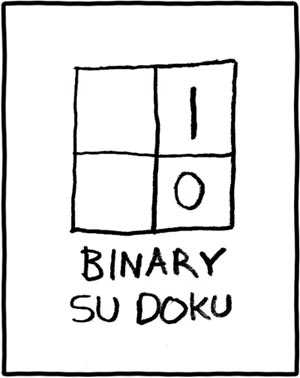
\includegraphics[width=3cm]{bilder/su_doku.png}\\
    }
}


%%%%%%%%%%%%%%%%%%%%%%%%%%%%%%%%%%%%%%%%%%%%%%%%%%%%%%%%%%%%%%%%%%%%%%%%%%%%%
\chapter{Studiengänge}
\section{Bachelor Allgemein}
Der Bachelor ist in den ersten Semestern sehr stark von Pflichtvorlesungen
geprägt, die kaum Wahlmöglichkeiten lassen. Gerade die ersten zwei Semester
sind in der Regel mit den Grundvorlesungen gut gefüllt. Ab dem dritten Semester
ist es dann aber meist möglich, euren Interessen nachzugehen.
Ein Bachelor lässt sich in drei bis vier Bereiche einteilen: Pflichtbereich,
Wahlpflichtbereich und Übergreifende Kompetenzen; im Bachelor Physik kommt noch
der Wahlbereich hinzu.
Der Pflichtbereich dient dazu, euch die Grundlagen eures Fachs beizubringen und
euch mit der fachlichen Methodik vertraut zu machen.  Im Wahlfpflichtbereich
vertieft ihr dann eure Kenntnisse und spezialisiert euch oft auf ein Gebiet. Im
Bereich Übergreifende Kompetenzen geht es um Soft- und Social Skills, aber auch
um fachlich übergreifendes Wissen.  Im Wahlpflichtbereich könnt ihr
schliesslich all das einbringen, was euch Spaß macht und nicht durch einen der
anderen Bereiche abgedeckt ist.

Die verschiedenen Veranstaltungen, die ihr während eures Studiums besucht, sind
in sogenannte Module gegliedert. Nach Definition ist ein Modul eine „thematisch
und zeitlich abgeschlossene Lehr- und Lerneinheit“. Ihr müsst euch allerdings
nicht lange mit dieser doch etwas umständlichen Formulierung befassen. Für euch
ist ein Modul nämlich nichts anderes als eine Vorlesung, die meist mit einer
schriftlichen Prüfung abgeschlossen wird, oder ein Seminar, in dem die Prüfung
aus einem Vortrag zu einem der Seminarthemen. Hin und wieder können euch auch
Module begegnen, die aus mehreren Veranstaltungen bestehen. Dann müsst ihr zum
Abschließen des Moduls eben nicht nur eine Prüfung bestehen oder einen Vortrag
halten, sondern eben alle\footnote{rechtlich heißt es zwar "ein Modul, eine
Prüfung", aber man kann da Ausnahmen machen.} Verstaltungen des Moduls bestehen.

Um den Stoff einer Vorlesung über das Semester hin zu vertiefen, gibt es in
fast allen Vorlesungen jede Woche einen Übungszettel mit Aufgaben zum aktuellen
Thema. Diese Zettel sind einerseits gut, um den Vorlesungsstoff aufzuarbeiten
und anzuwenden, andererseits braucht ihr auf den Zetteln in der Regel 50\% der
Punkte, um überhaupt zur Klausur zugelassen zu werden. Wie genau das dann
funktioniert, wird euch in den einzelnen Vorlesungen am Anfang jedes Semesters
ausführlich erklärt.

Für bestandene Module bekommt ihr dann Leistungspunkte (LP)\footnote{manchmal
auch Credit Points (CP) genannt}, von denen ihr in eurem Studium insgesamt 180
sammeln müsst (mit einigen Bedingungen verknüpft), um euren Bachelor zu
bekommen. Die Anzahl der Punkte, die ein Modul gibt, berechnet sich aus dem
„Workload“ einer Vorlesung. Das ist der Arbeitsaufwand, den eine Vorlesung und
die dazugehörige Übung mit sich bringt. Zum einen Teil ist das also Zeit, die
ihr in der Vorlesung und in den Übungen sitzt, aber auch die Zeit, die ihr für
das Vor- und Nachbereiten der Vorlesung und für das Rechnen des zugehörigen
Zettel braucht. Dabei entspricht ein LP in etwa 30 Stunden Arbeit im Semester,
also gute zwei Stunden pro Woche. Da es natürlich stark von euch abhängt, wie
lange ihr für das alles braucht und wie viel Zeit ihr wirklich investieren
wollt, kann das nur eine grobe Abschätzung sein, ist aber eine gute
Orientierung, wenn ihr überlegt, wie viel ihr euch im Semester aufbürden wollt.

\section{Bachelor Angewandte Informatik}
\sidebar{
    \centering
    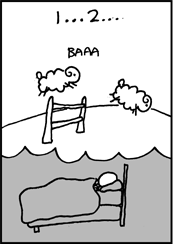
\includegraphics[width=3cm]{bilder/cant_sleep_1.png}\\\vspace{13mm}
    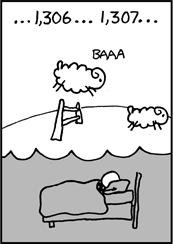
\includegraphics[width=3cm]{bilder/cant_sleep_2.png}\\\vspace{13mm}
    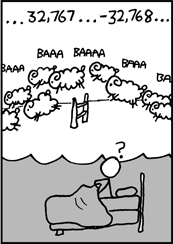
\includegraphics[width=3cm]{bilder/cant_sleep_3.png}\\\vspace{13mm}
    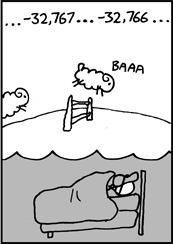
\includegraphics[width=3cm]{bilder/cant_sleep_4.png}
}

Im ersten Semester hört ihr die Informatikvorlesungen „Einführung in die Praktische Informatik“
und „Einführung in die Technische Informatik“ sowie eine Mathematikvorlesung.
Auch ist ein Programmierkurs Pflicht, in dem grundlegende Fertigkeiten in C++ vermittelt werden
sollen. Außerdem nehmt ihr an einem, von der Fakultät organsierten Mentoringprogramm, teil -- das Modul
heißt „Einführung in das Studium“ --, das euch den Einstieg ins Studium erleichtern soll.

In „Einführung in die Praktische Informatik“ (auch „Informatik~I“ genannt) sollt ihr Programmieren
und andere Grundfertigkeiten lernen. Ihr sollt einen Überblick über verschiedene Grundkonzepte der
Informatik und Grundkenntnisse in einer oder mehrerer Programmiersprachen bekommen.

Die „Einführung in die Technische Informatik“ („Informatik~II“) soll euch Kenntnisse über den
grundsätzlichen Aufbau und Funktionsweise von Rechnern vermitteln. Ihr lernt Schritt für Schritt,
angefangen bei Logik und einfachen Schaltungen, wie ein Prozessor funktioniert.

In den späteren Vorlesungen werden einzelne Themengebiete eröffnet und vertieft, die Namen der
Vorlesungen sprechen zum größten Teil für sich, zum Beispiel „Datenbanken“ oder „Betriebssysteme
und Netzwerke“.

Das Informatikstudium in Heidelberg beinhaltet einen in Vergleich zu anderen Universitäten hohen
Anteil an Mathematik. Ihr könnt von Anfang an entscheiden, welche Art der Mathematikausbildung ihr
erhalten möchtet. Ihr habt die Wahl zwischen mehreren Varianten.

In der ersten Variante hört ihr die Vorlesungen Lineare Algebra I (im 1.
Semester) und Analysis I (im 3. Semester). Alternativ könnt ihr als Ersatz für
die „Lineare Algebra I“ und die „Analysis I“ im ersten und zweiten Semester die
Veranstaltungen „Mathematik für Informatiker I und II“ hören.  Diese
Vorlesungen soll den Informatikstudierenden speziell die Mathematikkenntnisse
vermitteln, die sie in ihrem späteren Studium brauchen werden. Diese
Veranstaltung ist relativ neu, sie bietet aber trotzdem solide
Mathematikgrundlagen und den Bezug zur Informatik.

Hinzu kommen noch die Vorlesung Einführung in die Numerik und mindestens ein
Mathematikmodul eurer Wahl, wobei mindestens Analysis 2, Mathematische Logik
oder Einführung in die Wahrscheinlichkeitstheorie und Statistik belegt werden
muss.  Maximal dürft ihr aber insgesamt 5 Mathematikvorlesungen belegen, d.\
h.\ zu den oben beschriebenen Modulen dürft ihr maximal ein weiteres
Mathematikmodul belegen.

Die Mathematikmodule unterscheiden sich stark von der Schulmathematik,
unterschätzt den Aufwand für die Vorlesungen nicht!  Wenn ihr schon wisst, dass
ihr euer Informatikstudium mathematisch ausrichten und weitere Mathematikmodule
hört, euch vielleicht später sogar im wissenschaftlichen Rechnen spezialisieren
möchtet, ist die Variante mit Linarer Algebra I und Analysis I empfehlenswert.

Zum Thema Prüfungen und Prüfungswiederholungen: Um in den Vorlesungen
Creditpoints (meisten mit CP oder LP abgekürzt) zu bekommen, müsst ihr am Ende
in den meisten Fällen eine schriftliche Prüfung bestehen. Die genauen
Modalitäten, um überhaupt für die Prüfung zugelassen zu werden, legt die
Dozentin bzw.\ der Dozent am Anfang fest.  Informiert euch unbedingt genau,
worin die bestehen! Meist müsst ihr am Ende nur im Mittel 50 oder 60 Prozent
der Punkte auf den Übungszetteln erreichen, manchmal ist aber auch gefordert,
dass jeder Übungszettel bearbeitet wurde.

Ihr solltet euch auch bei jeder Veranstaltung genau darüber informieren, was
genau \emph{eine} Prüfung beinhaltet (z.\,B.\ Bestehen von einer von zwei
Klausuren). Insbesondere der letzte Teil ist wichtig, denn ihr könnt Prüfungen
grundsätzlich zweimal versuchen. Je nach Veranstaltung und Dozent/in
\emph{können} zwei Klausuren als eine Prüfung zählen, müssen aber nicht -- dann
würde jede geschriebene Klausur als ein Prüfungsversuch gelten. Wenn ihr aus
Gründen, die ihr nicht zu verantworten habt (wie krank sein), nicht an einer
\emph{Prüfung} teilnehmen konntet, erhöhen sich entsprechend eure Versuche.
Aber keine Panik -- auch wenn ihr in einer Vorlesung zum zweiten Mal die
Prüfung nicht bestanden haben solltest, seid ihr noch nicht exmatrikuliert: In
bis zu vier Fällen dürft ihr auf Antrag Prüfungen auch ein zweites Mal
wiederholen, dies gilt aber nicht für die Orientierungsprüfung und für die
Bachelorarbeit.

Denkt dran: Eine Klausuranmeldung ist eine Anmeldung zu einer Prüfung. Wenn ihr
euch sicher seid, sie nicht zu bestehen, überlegt euch lieber zweimal, ob ihr
euch anmeldet. Das Schöne an eurem Studiengang ist, dass die Noten der
Grundpflichtmodule nicht in eure Abschlussnote zählen, das heißt, dass auch
wenn die ersten Semester mit der ganzen Mathematik vielleicht etwas hart sind,
eure Abschlussnote darunter nicht unbedingt zu leiden hat.

Auch in Informatik gibt es eine sog. Orientierungsprüfung. Die besteht darin,
dass ihr den Schein der Vorlesung „Einführung in die Praktische Informatik“
bekommt. Diesen Schein müsst ihr spätestens am Ende des 3. Semester vorweisen
können.

Programmieren ist eine wichtige Fertigkeit. Und die werdet ihr nur teilweise an
der Uni lernen. Im Programmierkurs und in der Info I wird versucht, euch die
Konzepte näher zu bringen und in den Übungsaufgaben werdet ihr selber kleinere
Sachen programmieren müssen. Aber so lernt ihr letztlich nicht, wie man
„richtig“ programmiert.

Es gibt eine enorme Anzahl an Programmiersprachen und die meisten haben ihre
Daseinsberechtigung: um praktische Probleme zu lösen, akademisches Interesse
oder auch Unterhaltung. Es gibt diverse Paradigmen, nach denen
Programmiersprachen konzipiert sind und an der Uni werdet ihr nur die wenigsten
kennen lernen. Auch solltet ihr das System kennen, auf dem ihr arbeitet: solide
Kenntnisse von unixoiden Systemen sind immer Gold wert.

Die Uni hilft aber durchaus: Die „Einführung in die Praktische Informatik“
beinhaltet eine Art Programmierkurs, es gibt einen richtigen Programmierkurs,
der auch Pflicht ist, zur „Numerik 0“ gibt es praktische Übungen, in denen
ebenfalls programmiert wird. Eigeninitiative ist aber dennoch wichtig.

\vspace{-\parskip}

\section{Bachelor Mathematik}


\subsection{Das erste und zweite Semester}

In den ersten zwei oder drei Semestern hört ihr eure Grundvorlesungen und
einige Einführungsvorlesungen. Die Grundvorlesungen sind die Lineare Algebra I
und II, in denen ihr hauptsächlich Abbildungen zwischen Vektorräumen
betrachtet, und Analysis I und II, sowie Höhere Analysis. Dort behandelt ihr
Grenzwerte mit allem, was folgt, das heißt Differential- und Integralrechnung.

In der Prüfungsordnung wird in Anlage 1 und 2 noch einmal aufgelistet wie das
Studium aufgebaut ist. Auch das sind nur Vorschläge, wie ihr euer Studium im
Endeffekt einteilt, bleibt euch überlassen.

\subsection{Orientierungsprüfungen}

Orientierungsprüfungen sind Prüfungen, die bis Ende des dritten Semesters
bestanden sein müssen. In der Mathe sind das Analysis I und Lineare Algebra I
für Bachelor-Studis, bzw. Lineare Algebra I für Lehrämtler.  Diese Vorlesungen
müssen also im ersten Semester gehört werden.  Sollte man im ersten Anlauf, das
heißt in der ersten Klausur und in der Nachklausur nicht bestehen, ist das noch
lange kein Weltuntergang. Ihr seid damit nicht die Ersten und nicht die Letzten
an der Uni und sicher auch nicht die Einzigen in eurem Semester.  Es fallen
jedes Jahr etwa 50\%, mal mehr, mal weniger, durch diese Klausuren durch. Macht
euch deshalb also keinen Kopf! Ihr habt dann im WS darauf noch einen Versuch,
bestehend aus Klausur und Nachklausur. Der muss dann aber klappen, da euch
sonst die Exmatrikulation droht.

Die Einfühungsvorlesungen bestehen aus der Einführung in die praktische
Informatik, in die Numerik und in die Wahrscheinklichkeitstheorie und
Statistik.  In allen Vorlesungen müsst ihr Übungszettel lösen, die dazu dienen,
den Stoff zu vertiefen.  Ihr habt dann zu jeder Vorlesung Übungsgruppen und
einen Tutoren, die nicht nur eure Zettel korrigieren und sie mit euch
besprechen, sondern vor allem dazu da sind, euch zu helfen.  Tutoren werden
dafür bezahlt, eure Fragen zu beantworten, egal wie dumm sie euch in dem Moment
vorkommen, und machen das auch gerne.  Auch die anderen Studis verstehen meist
nicht mehr als ihr, sehr wahrscheinlich haben sie ähnliche Fragen.  Sucht euch
am besten am Anfang eine Gruppe von Kommilitonen, mit denen ihr gut rechnen und
überlegen könnt, damit ihr die Zettel nicht alleine bearbeiten müsst.  Abgeben
sollt ihr sie auch nicht alleine, sondern im Allgemeinen zu zweit.

Zusätzlich kann im zweiten Semester ein Proseminar besucht werden. Das
Proseminar setzt eine aktive Teilnahme voraus und wird mit einem mündlichen
Vortrag abgeschlossen, evtl mit zusätzlicher schriftlicher Ausarbeitung.  Der
Vortrag ist eine sehr gute Möglichkeit LaTeX zu lernen.  LaTeX ist ein
Programm, um pdf-Dokumente zu schreiben, ihr werdet es in eurem Mathestudium
noch häufig brauchen und wie heißt es so schön: Früh übt sich, wer ein Meister
werden will (Schiller).


Im Mathebachelor müsst ihr ein Anwendungsgebiet wählen, welches ein Fach eurer
Wahl sein kann, allerdings gibt es nur für Informatik, Physik, Astronomie,
Biologie, Chemie, Wirtschaftswissenschften und Philosophie eine in der
Prüfungsordnung festgelegte Regelung, alle andern Fächer könnt ihr nur nach
Rücksprache mit dem Prüfungsausschuss als Anwendungsgebiet wählen.

\subsection{Schlusswort}

In den ersten beiden Semestern kann es passieren, dass eure Noten nicht so gut
sind, wie ihr das vielleicht gerne hättet oder aber gewohnt seid.  Das ist aber
noch lange kein Weltuntergang und auch noch kein Grund, das Studium
abzubrechen, wenn ihr Spaß an Mathematik habt. Mathematik an der Uni ist etwas
ganz anderes als die Mathematik, die man aus der Schule kennt.  Es wird auch
gerne die Tatsache unterschätzt, dass man plötzlich in einer ganz neuen
Situation ist, eine für die meisten fremde Stadt, neue Leute, ein ganz anderes
System als die Schule.  Man muss sich erstmal an die geänderten äußeren
Umstände gewöhnen und das braucht Zeit.  Auch die Klausuren sind nicht so
schlimm, wie es einem am Anfang vorkommen mag.  Ihr habt im Regelfall eine
zweite Chance, wenn ihr durch die erste durchfallt.  Sollte auch der zweite
Anlauf nicht klappen, dann könnt ihr die Vorlesung im nächsten Jahr noch einmal
hören. Es ist also nichts verloren.

Wenn ihr sonst über irgendetwas stolpert, gibt es immer noch die Fachschaft,
die euch gerne weiterhilft. Ihr könnt entweder persönlich bei uns vorbei kommen
oder eine Mail schreiben. Wir versuchen dann, euch zu helfen, wo es nur geht.


\subsection{Alle weiteren Semester}

Der weitere Verlauf des Studiums kann von jedem ganz individuell gestaltet
werden.  Man kann sich dabei nach einem der Stundenpläne, die auf der Homepage
der Fakultät zu finden sind, richten. Bei der Frage, welche Vorlesungen und
Veranstaltungen ihr belegen müsst und könnt, helfen euch Modulhandbauch,
Prüfungsordung und Homepage der Fakultät.

Gerade am Anfang eures Studium werdet ihr möglicherweise nicht so gute Noten
haben, da ihr euch erst an die zunächst noch sehr ungewohnte Uni-Mathe gewöhnen
müsst. Aber verzweifelt nicht daran, denn ihr werdet euch schnell daran gewöhnt
haben und dann wird aus Linearer Algebra I und II sowie Analysis I und II  auch
nur die jeweils bessere Analysis- und die bessere Lineare-Algebra-Note in eurem
Bachelor berücksichtigt.

\subsection{Prüfungsordnung}

In der Prüfungsordnung (PO) findet ihr alle wichtigen Informationen darüber,
welche Veranstaltungen gehört werden müssen, welche Prüfungen wann und wie
abgelegt werden müssen und wie euer Studium sonst geregelt ist.  In der
Prüfungsordnung könnt ihr nachschlagen, welche Pflich- und
Wahlpflichtveranstaltungen es gibt und wieviele und welche
Wahlpflichtveranstaltungen gehört werden müssen (Anlage 1 und 2).  Im
Modulhandbuch findet ihr kurze Beschreibungen der Veranstaltungen und welche
Vorkenntnisse für sie empfohlen werden.  Neben Pflicht- und Wahlpflichtmodulen
gibt es noch das Anwendungsgebiet und fachübergreifende Kompetenzen.  Über
letztere braucht ihr euch keine großen Sorgen machen, die hat man meist
schneller als ihr denkt. Möglichkeiten sind hier Praktika, Auslandssemester,
Sprachkurse, die das Zentrale Sprachlabor der Universität Heidelberg anbietet,
Vorlesungen anderer Fächer und so weiter.  Bereits 8 der 20 Leistungspunkte für
fachübergreifende Kompetenzen sind bereits in andere Veranstaltungen
integriert.  In Anlage 3 der PO findet ihr mehr Informationen darüber, wie und
wann ihr diese Leistungspunkte erwerbt.


\subsection{Anwendungsgebiet}

Zusätzlich zum puren Mathematik-Studium habt ihr das Anwendungsgebiet, was ein
Fach eurer Wahl sein kann.  In der Prüfungsordnung gibt es aber nur für die
Fächer Informatik, Physik, Astronomie, Biologie, Chemie,
Wirtschaftswissenschaften und Philosophie eine feste Regelung. Nach Rücksprache
mit dem Prüfungsausschuss können jedoch auch andere Fächer angerechnet werden.
Habt ihr zum Beispiel ein Studium vorher abgebrochen, kann das oft als
Anwendungsgebiet angerechnet werden.  Die meisten der oben genannten Fächer
fangen laut Musterstudium in eurem dritten Semester an, die interessanten
Informatikvorlesungen sind dagegen im Sommersemester.  Niemand wird euch daran
hindern euer Anwendungsgebiet schon im ersten Semester zu beginnen,
unterschätzt jedoch die Arbeitbelastung des Grundstudiums nicht.

Ganz am Ende erwarten auch dann noch ein weiteres Seminar, welches häufig als
Grundlage für die Bachelorarbeit verwendet wird, und dann die Bachelorarbeit.


\section{Bachelor Physik}

\subsection{Erstes Semester}

Das erste Semester ist, verglichen mit späteren Semestern, sehr stark durchstrukturiert, was euch den Wechsel von der Schule an die Uni erleichtert, jedoch auch nicht besonders viele Freiheiten lässt.
Allgemein werdet ihr bis ins vierte Semester im Pflichtprogramm je eine Experimentalphysik und eine Theoretische Physik Vorlesung besuchen, wobei im fünften Semester noch die Experimentalphysik V folgt. Zusätzlich dazu hört ihr an Mathe im ersten Semester die Lineare Algebra I und wenn ihr wollt auch die Analysis I; aber zur Mathe später mehr.

Das ganze Semester über werdet ihr jede Woche in jeder Vorlesung, die ihr hört, einen Übungszettel bekommen, den ihr dann auf die nächste Woche lösen sollt. Diese dienen zum Einüben des in den Vorlesungen behandelten Stoffes und zugleich als Klausurzulassung. Man benötigt meistens insgesamt 50 - 60 \% der Gesamtpunktzahl auf allen Zetteln, aber wenn es nur um ein paar Punkte geht, sind die Tutoren meistens kulant. Wenn euer Tutor den Eindruck hat, ihr verschwendet nicht nur einen Prüfungsversuch mit der Klausur, lässt er euch meistens zu. Macht euch darum aber erstmal keinen Kopf, wenn man am Ball bleibt, ist das überhaupt kein Problem, ihr müsst sie ja nicht alle alleine lösen.

\subsubsection{Orientierungsprüfung}

Die Orientierungsprüfung ist eine Prüfung, die ihr bis zum Ende des 3. Semesters bestehen müsst, um weiterhin Physik studieren zu dürfen. Im Bachelor Physik ist dies die ganz normale Klausur in der Experimentalphysik I. Dort werden meist sehr schulnahe physikalische Grundlagen der Mechanik behandelt. Macht euch also keine Sorgen. Das schafft ihr!

\subsubsection{Basiskurs}

Der Basiskurs beginnt, wie ihr wahrscheinlich schon wisst, in der letzten Vorkurswoche und soll euch den Einstieg in das Studium erleichtern. Dabei werden euch sogenannte Schlüsselkompetenzen beigebracht, die euch unter anderem in Zeitmanagement, Literatursuche und das Textsatzsytem \LaTeX{} einführen. Auch wenn ihr vermutlich schon einiges davon kennt, ist es doch ganz nett, nochmal alles kompakt zu sehen und vor allem dabei neue Menschen und vielleicht auch spätere „Zettelpartner“ kennenlernen zu können. Leider ist die Qualität des Kurses oft stark abhängig von eurem Tutor. Ihr müsst also für euch bestimmen, wie viel ihr aus diesem Kurs mitnehmt. Bedenkt, der Tutor bekommt Geld für diesen Kurs, ihr dürft also auch etwas von ihm erwarten. %(Stimmen die Inhalte des Basiskurses? Ja, die stimmen.)
\subsubsection{Analysis vs. Höhere Mathematik für Physiker}
\label{mathephysik}

Die Mathematikausbildung für Physiker*innen sieht vor, dass ihr die Lineare Algebra I im ersten Semester hört. Laut Modulhandbuch kann man sich dann vor dem zweiten Semester entscheiden, ob man mit Analysis II und III (was auch die Mathematiker*innen hören) oder mit Höhere Mathematik für Physiker (HöMa) II und III weitermacht.\\

Was spricht für Höhere Mathematik für Physiker (HöMa)?\\
Die Vorlesung ist extra auf euch als Physiker*innen zugeschnitten und legt ihren Schwerpunkt auf die Vorlesungen Analysis 1-3 in strafferer Form. Während Mathematikvorlesungen einer gewissen
Freiheit unterliegen und es durchaus vorkommen kann, dass die/der Dozent*in einen Schwerpunkt auf ihr/sein Forschungsgebiet legt, hört ihr in HöMa größtenteils auch nur jene Dinge, die in der Physik auch verwendet werden. Außerdem kommen Beispiele gerne aus der Physik und liegen euch deshalb vielleicht näher. Trotzdem handelt es sich nicht um eine Schmalspurversion, sondern um eine vollwertige Mathematikvorlesung, die auch für zukünftige Theoretiker nicht ungeeignet ist.\\

Was spricht für die Analysis?\\
Die Analysis bietet als eine für Mathematiker*innen konzipierte Veranstaltung eine präzisere Formulierung der Definitionen, Sätze und insbesondere Beweise. Somit wird es möglich die mathematischen Hintergründe in der Physik besser zu durchdringen und weitergehende Verbindungen der Gebiete zu erkennen. Dieses tiefere Verständnis kann unter anderem in der theoretischen Physik oder auch in weiterführenden Matheveranstaltungen von Vorteil sein und lässt euch insgesamt mehr Freiheiten im weiteren Studienverlauf, besonders bezüglich der Mathematik.
Zudem ist je nach Dozent*in und Forschungsbereich auch eine gewisse Schwerpunktlegung (vor allem in der Analysis III) möglich.\\

Auf den ersten Blick mag es verwundern, dass man in die Analysis II einsteigen soll, ohne die erste Vorlesung dazu gehört zu haben. Dies ist theoretisch zumindest möglich, jedoch vermutlich mit ein wenig Mehraufwand verbunden. Trotzdem können mathematisch Ambitionierte natürlich auch die Analysis I im ersten Semester hören, da diese eine schöne Einführung in den Themenbereich Analysis und die damit verbundenen Methoden darstellt. Das kann einem vor allem in weiterführenden Vorlesungen weiterhelfen; auch wird es eine große Erleichterung für die Analysis II sein, wenn man schon ein wenig mehr mit der Materie und dem Dozenten vertraut ist.
Andererseits werdet ihr mit dem Kursprogramm auch so schon stark ausgelastet sein. Wenn ihr es mit vier Vorlesungen versuchen wollt, solltet ihr euch nach zwei bis drei Wochen entschieden haben, ob ihr das im ersten Semester durchhaltet oder nicht, da es für den Übungsbetrieb ziemlich blöd ist, wenn in der Mitte des Semesters viele Leute aussteigen.


\subsection{Weiteres Studium}

Euer weiteres Studium sieht, wie oben kurz angedeutet, so aus, dass ihr immer ein Grundgerüst an Vorlesungen habt und euch darum herum andere Vorlesungen und Seminare selbst auswählen könnt. Die Experimentalphysikvorlesungen sind bis zum fünften Semester und die theoretischen bis zum vierten Semester Pflicht. Hinzu kommen im zweiten und dritten Semester entweder die Höhere Mathematik für Physiker (HöMa) II und III, oder die Analysis II und III. Ansonsten seid ihr jedoch bis auf ein Pflichtseminar, das ihr aus einem relativ großen Topf an Seminaren auswählen könnt und den Pflichtpraktika frei alles zu hören, was euch so in den Sinn kommt. Ihr müsst einzig darauf achten, dass ihr in den einzelnen Bereichen ausreichend „Punkte sammelt“: Im Wahlpflichtbereich sind das 14 CP, bei den Übergreifenden Kompetenzen 19 CP und im Wahlbereich bis zu 17 CP. Nutzt frühzeitig die Gelegenheit Veranstaltungen zu besuchen, die euch interessieren, dann macht das Studium gleich doppelt so viel Spaß!

\subsection{Wahlbereich, Wahlpflichtbereich und Übergreifende Kompetenzen}

Im Laufe Eures Bachelorstudiums müsst ihr ggf. ein oder zwei Wahlfächer belegen, welche ihr aus einem recht weit gefächerten Angebot wählen könnt. Diese Wahlfächer müssen auch nicht zwingendermaßen aus Bereichen der Physik kommen, sondern können z.B. Mathe, Chemie oder Philosophie sein. Was ihr alles für Möglichkeiten habt, könnt ihr genauer in der Prüfungsordnung nachlesen und selbst Fächer, die dort nicht aufgezählt sind, lassen sich möglicherweise nach Absprache mit dem Prüfungsausschuss auch anrechnen lassen.\\

Der Wahlpflichtbereich besteht, im Gegensatz zum Wahlbereich und den Übergreifenden Kompetenzen, aus vertiefenden oder weiterführenden Physikveranstaltungen. Schaut doch einfach in das Vorlesungsverzeichnis im LSF und sucht euch interessante Vorlesungen oder auch Seminare aus. Besonders Seminare können viel Spaß machen, da diese zwar oftmals viel selbstständiges Arbeiten verlangen, aber oft auch forschungsnäher sind als Vorlesungen. Zudem findet ihr auch Anregungen dazu in der Prüfungsordnung und im Modulhandbuch.\\

Der Bereich Übergreifende Kompetenzen soll euch ein wenig dazu bewegen fachunabhängige Kompetenzen zu erlernen. Darunter fallen der mathematische Vorkurs, der Basiskurs, sowie alle als „Überfachliche Kompetenzen“ gekennzeichneten Module der Mathematik, Informatik und den Naturwissenschaften. Außerdem lassen sich oft nach Rücksprache mit dem Prüfungssekretariat auch weitere Veranstaltungen anrechnen lassen, wie zum Beispiel Sprachkurse, Programmierkurse, usw.\\

Allgemein gilt: Versucht, möglichst früh Dinge aus Gebieten, die euch wirklich interessieren, zu hören; denn das sind die Fächer die euch auch wirklich Spaß machen und ihr erlangt ein möglichst breites, und vor allem tiefes Wissen, welches euch bei eurer Bachelorarbeit und vermutlich auch sonst zugutekommt.


\subsection{Prüfungen und Noten}

Es wird euch sicher freuen zu hören, dass eine nicht bestandene Klausur nicht gleich das Ende für euer Studium bedeutet. Im Grunde ist die Wiederholungsregelung sogar recht studifreundlich; so habt ihr in jedem Modul zwei Versuche, wobei in der Regel ein Versuch aus einer Klausur und, wenn nötig, der dazugehörenden Nachklausur besteht. Darüber hinaus habt ihr für euer Studium noch zwei sogenannte Joker, die euch jeweils einen dritten Versuch geben, falls die zwei regulären nicht reichen sollteni (dies gilt nicht für eure Orientierungsprüfung, welches die Prüfung in der Experimentalphysik I darstellt). Darüber hinaus ist für euch recht interressant, dass es die Möglichkeit gibt, zwei Noten aus unterschiedlichen Bereichen der tendenziell schlechteren Pflichtmodule zu streichen. Macht euch also nicht zu viele Gedanken darüber, wenn eure Noten zunächst nicht ganz so gut sind. Auch könnt ihr jederzeit zusätzlich gehörte Module in den Zusatzqualifikationenbereich verschieben, wenn ihr diese nicht benötigt, euch entsteht also kein Nachteil dadurch, dass ihr mehr hört, als ihr müsst.\\

Sonst ist noch zu erwähnen, dass ihr, um in Heidelberg in den Master zugelassen zu werden, eine Bachelornote von 2,9 oder besser braucht. Das war bisher, so wurde uns versichert, aber noch nie ein Problem, für Heidelberger Studis, der Notenschnitt lag im Bachelor bei etwa 1,7.

\subsection{Prüfungsordung und Modulhandbuch}

Immer dann, wenn sich euch Fragen zu eurem Studium stellen oder ihr euch einfach über den weiteren Studienverlauf informieren wollt, sind die ersten Anlaufstellen die Prüfungsordung und das Modulhandbuch. In der Prüfungsordung ist formal geregelt, wie der Studienablauf, die Prüfungen und die Anrechenbarkeit von Modulen aussehen. Das Modulhandbuch wiederum ist im Großen und Ganzen eine Auflistung der in der Physik (und benachbarten Gebieten) angebotenen Veranstaltungen. Zurzeit findet ihr beide Dokumente auf der Hauptseite des Bachelors Physik. Leider ist das Modulhandbuch oft nicht ganz aktuell, falls euch Verbesserungen auffallen, meldet euch einfach bei uns.\\

Ansonsten könnt ihr auch gerne zu uns in die Fachschaft auf eine Tasse Kaffee oder Tee vorbeikommen. In vielen Fällen können wir euch auch weiterhelfen.

\section{Die 50\%-Bachelor-Studiengänge (Lehramt)} % Dereinst "Lehramt allgemein"
\label{lehramt_allg}

Lehramtsstudiengang, Staatsexamen, Referendariat -- so ging es vor 2015 zurück
an die Schule.  Die ersten beiden Schritte haben sich nun verändert, denn die
Umstellung der Studiengänge in Deutschland auf das zweistufige
Bachelor-Master-System macht auch vor dem Lehramt in Baden-Württemberg nicht
halt. Und daher heißt es jetzt: Doppel-Fachbachelor, Master of Education,
Referendariat. Andernorts heißt es manchmal auch: Bachelor of Education, Master
of Education, Referendariat. Das zweite Konzept versucht, das alte
Lehramtsstudium soweit wie möglich zu erhalten, während in Heidelberg mit dem
heiEDUCATION-Konzept eine Umstellung auf das Erste vorgenommen wird -- mit dem
Nebeneffekt, dass es künftig auch möglich sein wird, Informatik, Mathematik und
Physik als 50\%-Bachelorstudiengang zu studieren.

\subsection{heiEDUCATION}

heiEDUCATION ist ein von Universität und Pädagogischer Hochschule (PH)
Heidelberg gemeinsam entwickeltes Konzept um „Heidelberg zu einem Ort
exzellenter Lehrerbildung
auszubauen“\footnote{\url{http://www.hei.education/de/hauptmenue/startseite/}}.
Exzellente Lehrerbildung bedeutet dabei folgendes:

Lehramtsstudierende absolvieren zunächst parallel zwei
50\%-Bachelorstudiengänge an der Universität Heidelberg. Diese Studiengänge
haben fast keinen Lehramtsbezug, lediglich vereinzelte Veranstaltungen für
Fachdidaktik und Bildungswissenschaften können belegt werden. Vorgesehen ist,
dass man im 6. Semester in einem der beiden Fächer eine Bachelorarbeit
schreibt. Während diesem Studium lernt ihr also alle nötigen fachlichen
Kompetenzen für das Lehramt.

Anschließend kann man wahlweise auf den „Master of Education“ oder einen
Fachmaster in einem der beiden Fächer wechseln. Der „Master of Education“ wird
von der PH angeboten und die soll die notwendigen Kompetenzen für das
Unterrichten vermitteln.  Diese sogenannte „Polyvalenz“ hat den Vorteil, dass
dass Lehramtsstudierende bis zum 6. Semester Zeit für die Entscheidung zwischen
Fach- und Lehramtsausbildung haben, und die 50\%-Bachelorstudiengänge eine
interessante Option für Studierende bieten, die an zwei Fächern großes
Interesse haben.

Da dieses neue Konzept von denen, die die Umstellung zu verantworten haben,
reichlich positiv gesehen wird, sollen an dieser Stelle einige skeptische Worte
nicht fehlen:

Zunächst ist der Master of Education momentan noch ein recht abstraktes
Konzept, das erst in den kommenden Semestern Gestalt annehmen wird. Zwar steht
beispielsweise schon fest, dass das Praxissemester im Rahmen des Master of
Education weiterbestehen wird, vieles andere ist aber noch offen. Außerdem muss
man Lehramtsstudierenden ganz klar sagen: Ihr werdet in euren ersten Semestern
kaum auf eure spätere Berufspraxis vorbereitet. Sicherlich ist ein tiefes
Verständnis von Inhalten auch jenseits des Schulstoffes wichtig, um später an
Schulen gut unterrichten zu können. Doch die tatsächliche Planung von
Unterricht, der Schritt vom eigenen Verständnis von Inhalten hin zur Fähigkeit,
anderen das Verständnis von Inhalten zu ermöglichen, geschieht in diesem
Konzept erst spät. Daher der Appell an all diejenigen, die am liebsten sich
schon morgen vor eine Schulklasse stellen und unterrichten würden: Habt Geduld
und beißt euch durch!

\subsection{Bachelor of Everything\dots}

\dots oder zumindest mal in zwei Fächern gleichzeitig: Einer der Vorteile
dessen, wie in Heidelberg das Lehramt umgestellt wurde, ist die hinzugewonnene
Möglichkeit, zwei Fächer zu einem Bachelorstudiengang zu kombinieren
(„Doppelbachelor“) und sich damit für beide Fach-Masterstudiengänge zu
qualifizieren. Zum einen hat man so weitere zwei bis drei Jahre Zeit, sich
zwischen den Gebieten zu entscheiden. Zum anderen kann man diesen Studiengang
wählen, wenn man zum Ziel hat, an den Grenzflächen zweier Wissenschaften zu
arbeiten. Physikalische Chemie, Wissenschaftliches Rechnen und Mathematische
Physik sind hier gute Beispiele.

Es muss allerdings darauf hingewiesen werden, dass man sich die größere
fachliche Breite auf Kosten der Spezialisierung in den Fächern aneignet. Das
kann je nach Fach bedeuten, dass man im Fachmaster später noch Grundlagen
aufholen muss, um dieselbe fachliche Tiefe zu erreichen wie die
100\%-Bachelor-Studierenden. Dazu kommt, dass man nur eine Bachelorarbeit
schreibt, für die man zwischen den Fächern wählen muss. Teilweise ist an dieses
Wahl die Zulassung für den Fach-Master geknüpft, teils treffen Fächer
Einschränkungen auf bestimmte Fächerkombinationen. Es ist für Studierende des
Doppelbachelors daher besonders wichtig, schon frühzeitig sich über die
formalen Regelungen in ihren Fächern zu informieren. Dies könnte beispielsweise
eine überblicksartige Lektüre der Prüfungsordnungen sein. Auch die Hinweise für
die Fächer Informatik, Mathematik und Physik in den folgenden Abschnitten sind
vermutlich hilfreich, doch es können dort natürlich nicht alle möglichen
Fächerkombinationen diskutiert werden.


%TODO: \subsection{Immatrikulation für das Lehramtsstudium}
% -- davon habe ich keine Ahnung...
%
% Früher stand da mal:
% \subsection{Immatrikulation für das Lehramtsstudium}
%
% Grundsätzlich immatrikuliert man sich im Staatsexamensstudiengang Lehramt
% immer in mindestens zwei Hauptfächern. Gegebenenfalls kann nach der
% Zwischenprüfung in den Hauptfächern noch ein drittes Fach -- ein sogenanntes
% Erweiterungsfach -- hinzukommen.
%
% Aber Vorsicht! Manche Fächer können nicht auf Lehramt studiert werden, andere
% Fächer nur in bestimmten Kombinationen. Obwohl das Studentensekretariat darauf
% achten sollte, kommt es immer wieder vor, dass Leute mit „falschen“
% Kombinationen immatrikuliert werden. Seht auf jeden Fall nochmal selber nach:
% Welche Fächerkombinationen in Baden-Württemberg auf Lehramt studiert werden
% können, entnehmt ihr einer Tabelle des Kultusministeriums, die ihr bei
% verschiedenen Beratungsstellen (meist auch online auf deren Webseite) einsehen
% könnt: Es gibt für jedes Fach eine eigene Lehramtsberatung sowie eine zentrale
% Beratung für Lehramtsstudierende durch das Oberschulamt; für
% rechtsverbindliche Auskünfte sollte man sich an letztere wenden.
%
% \emph{Achtung:} In anderen Bundesländern gelten andere Regelungen!
%
%
% Zur Immatrikulation für einen Lehramtsstudiengang muss eine Bescheinigung über
% die Ableistung eines sogenannten Orientierungspraktikums vorgelegt werden.
% Sofern diese noch nicht vorliegt, kann sie aber für eine begrenzte Zeit noch
% nachgereicht werden. Die konkrete Frist orientiert sich meist an den sonstigen
% Fristen der Immatrikulation, lest hierzu am besten auf der Seite des
% Studierendensekretariats nach oder ruft dort an (06221 -- 54\,54\,54).


\subsection{Modularisierung}

Die 50\%-Bachelorstudiengänge sind modularisiert, d.h. die Lerninhalte werden
in kleinen, abgeschlossenen Einheiten, sogenannten Modulen, vermittelt. Ein
Modul umfasst beispielsweise wöchentlich zwei Vorlesungen und eine Übung mit
Übungszetteln über ein Semester oder ein Praktikum. Auch die Bachelorarbeit ist
ein Modul. Oftmals werden Module sowohl von Studierenden des 100\%- und des
50\%-Bachelorstudienganges belegt. Alle Module werden mit Leistungspunkten (LP;
oder CP für „Credit Points“) versehen, die den Arbeitsaufwand messen sollen.
Dabei entspricht 1 LP ca. 25-30 Stunden Arbeit. Für einen Bachelor müssen
insgesamt 180 LP gesammelt werden. Die Gesamtnote des Bachelorabschlusses
ergibt sich aus den nach LP gewichteten Noten der Module.

\subsection{Fachdidaktik und Bildungswissenschaften}

Für die Zulassung zum Master of Education ist das Absolvieren von Modulen mit
insgesamt 20 Leistungspunkten für Fachdidaktik und Bildungswissenschaften
erforderlich. Welche Verantstaltungen hier so angeboten werden, ist uns leider
auch noch nicht ganz klar, aber da das zum einen „nur“ 20 Punkte, zum anderen
in den ersten Semestern vermutlich recht uninteressant ist, könnt ihr das
getrost auf euch zukommen lassen.

% TODO: Weitere Informationsangebote schaffen und kommunizieren

%%%%%%%%%%%%%%%%%%%%%%%%%%%%%%%%%%%%%%%
% KEEP THIS!!
%
% Sobald bekannt ist, wie der Master of Education aussehen wird, sollte es hier
% einen Abschnitt darüber geben. Insbesondere ist auf das Praxissemester
% einzugehen. Das wurde früher(TM) mal so beschrieben:
%
% \subsection{Praxissemester}
%
% Gemäß der Lehramtsprüfungsordnung müssen Lehramtsstudierende ein
% Schulpraxissemester absolvieren oder eine vergleichbare Schulpraxis (z.B.
% Assistant Teacher im Ausland) nachweisen.  Das Praxissemester soll -- so das
% Kultusministerium -- schon früh den Bezug zur Schulpraxis herstellen. (Dass
% für die Einführung aber auch Kostengründe gesprochen haben, ist kaum zu
% leugnen. Schließlich wird das Schulpraxissemester nicht bezahlt, im Gegensatz
% zu dem halben Jahr Referendariat, welches dadurch ersetzt wird.)  Das
% Praxissemester soll in der Regel nach dem dritten oder vierten
% Studiensemester, also gegen oder nach Ende des Grundstudiums absolviert
% werden. Empfehlenswert ist häufig das fünfte Fachsemester, wie es auch in den
% Studienordnungen der meisten Fächer vorgeschlagen wird. Letztlich könnt ihr
% aber den Termin frei wählen. Das Praxissemester dauert 13 Wochen – es beginnt
% zum Schuljahresbeginn im September und endet mit Beginn der Weihnachtsferien.
% Während des Praxissemesters besucht man nachmittags Kurse beim Staatlichen
% Seminar für Didaktik und Lehrerbildung, wo man etwas über Pädagogik und
% Fachdidaktik lernen soll.
%
% Ihr solltet bereits ein einführenden Vorlesung in Bildungswissenschaft sowie
% pro Fach eine Fachdidaktikveranstaltung besucht haben, bevor ihr in der Regel
% im 5. Semester ins Schulpraxissemester geht. Im Frühjahr, bis das kommende
% Semester startet, habt ihr eventuell die Möglichkeit Blockveranstaltungen zu
% belegen.
%
% Die Vergabe der Praktikumsplätze wird über das Internet geregelt -- nähere
% Infos dazu findet man auf der Homepage der jeweiligen Fakultät.
%%%%%%%%%%%%%%%%%%%%%%%%%%%%%%%%%%%%%%%


\subsection{Übersicht} %TODO: Punktezahlen überprüfen! %TODO: die Tabelle muss evtl. angepasst werden (Zeilenumbrüche)
Hier nochmal eine Übersicht über die Leistungspunkte, die im Lehramt, bzw. Doppelbachelor erbracht werden müssen:

\begin{table*}[htb]
	\centering

	\begin{tabular}{ll}
		\toprule
		Bereich  & Leistungspunkte\\
		\midrule
		Fach A, Fachstudium & 74\\
		Fach A, Fachdidaktik & \phantom{0}2\\
		\addlinespace
		Fach B, Fachstudium & 74\\
		Fach B, Fachdidaktik & \phantom{0}2\\
		\addlinespace
		Bildungswissenschaften oder Fachwissenschaften* & 16\\
		\addlinespace
		Bachelorarbeit (in einem der Fächer) & 12\\
		\bottomrule
	\end{tabular}

\end{table*}
Dabei sollten im mit * gekennzeichneten Teil Module in den
Bildungswissenschaften gewählt werden, wenn ein Übergang in den Master of
Education angestrebt wird, andernfalls können je nach Fach diese
Leistungspunkte durch fachwissenschaftliche Module erbracht werden.
     %\newpage %%%%%
%\Large\mathphyssubsubsec{Lehramt Informatik}\normalfont\small
\section{50\%-Bachelor Informatik (Lehramt)}
\sidebar{
	\centering
	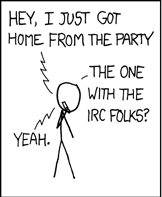
\includegraphics[width=3.5cm]{bilder/xkcd_responsible_behaviour_1.png}\\\vspace{10mm}
	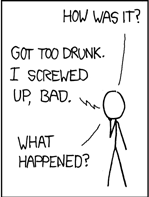
\includegraphics[width=3.5cm]{bilder/xkcd_responsible_behaviour_2.png}\\\vspace{10mm}
	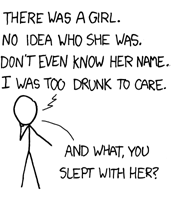
\includegraphics[width=3.5cm]{bilder/xkcd_responsible_behaviour_3.png}\\\vspace{10mm}
	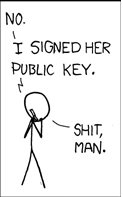
\includegraphics[width=3.1cm]{bilder/xkcd_responsible_behaviour_4.png}
}

Wenn ihr den 50\%-Bachelor Informatik studiert, sind zwei Fälle zu
unterscheiden: Entweder hört ihr in eurem zweiten Fach
Mathematik-Veranstaltungen oder ihr tut es nicht. Diese Unterscheidung rührt
daher, dass ihr in der Informatik auf jeden Fall etwas Mathematik können
solltet. Wenn ihr in eurem anderen Fach Mathe hört, habt ihr das aber schon da
abgedeckt und könnt euch in dieser Hälfte eures Bachelors ganz auf die
Informatik konzentrieren.

Auf jeden Fall hört ihr im ersten Semester \hyperref[info1]{„Einführung in die
Praktische Informatik“ (Info 1)} und den Programmierkurs. Hier ist besonders
die erste Veranstaltung wichtig, da es euere Orientierungsprüfung in Informatik
ist. Im zweiten Semester solltet ihr dann in Informatik die „Einführung in die
Theoretische Informatik“ \footnote{„Theo“ kann zu Verwirungen mit Physikern
führen, da diese das als „Theoretische Physik“ verstehen} und „Algorithmen und
Datenstrukturen“ (AlDa) hören. Im Dritten Semester macht sich der Unterschied,
ob ihr in eurem zweiten Fach Mathe hört oder nicht, bemerkbar, da ihr hier
„Mathematik für Informatiker 1“ (MafIn 1)  hören sollt.  Wenn ihr aber bereits
andere Matheveranstaltungen bestanden habt, könnt ihr beim Prüfungsausschuss
beantragen, dass ihr stattdessen ein weiteres Info-Modul aus den
Wahlpflicht-Veranstaltungen hören könnt.  Ausserdem ist vorgesehen das ihr im
Dritten Semester die „Einführung in die Technische Informatik“ (ITE oder
Technische Info)\footnote{dafür hat leider noch niemand eine schön Abkürzung
gefunden} hört.  Im Vierten und Fünften Semester stehen dann „Betriebssysteme
und Netzwerke“ (BeNe), „Software Engineering“ (ISW) und ein Proseminar auf dem
Plan. Im sechsten Semester müsst ihr dann neben der Bachelorarbeit, die ihr in
einem eurer beiden Fächer schreibt, noch „Datenbanken 1“ (IDB1) hören. Hinzu
kommen dann noch ein Anfängerparktikum und ein Seminar. Falls ihr nach dem
Bachelor den „Master of Education“ machen wollt, müsst ihr das Proseminar und
das Anfängerpraktikum im Themenbereich „Informatik und Gesellschaft“ (IuG)
machen.  Da im Seminar und Proseminar und Seminar schon LP als
„Fachübergreifende Kompetenzen“ (FÜK) vergeben werden habt ihr nun noch 4 LP
die ihr mit einer FÜK Veranstaltung eurer Wahl holen könnt.

Ihr solltet euch bei jeder Veranstaltung genau darüber informieren, was ihr
benötigt, um zur Prüfung zugelassen zu werden (z.B. 50\% auf den Übungszetteln)
und was genau \emph{eine} Prüfung beinhaltet (z.\,B.\ das Bestehen von einer von
zwei Klausuren). Insbesondere der letzte Teil ist wichtig, denn ihr könnt
Prüfungen grundsätzlich zweimal versuchen. Je nach Veranstaltung und Dozent/in
\emph{können} zwei Klausuren als eine Prüfung zählen, müssen aber nicht -- dann
würde jede geschriebene Klausur als ein Prüfungsversuch gelten. Wenn ihr aus
Gründen, die ihr nicht zu verantworten habt (wie krank sein), nicht an einer
\emph{Prüfung} teilnehmen konntet, erhöhen sich entsprechend eure Versuche.
Wenn ihr alle \emph{Klausur}termine verpasst habt, kann die Klausur auch durch
eine mündliche Prüfung ersetzt werden. Sollte das bei euch mal der Fall sein,
fragt ihr jedoch am besten den/die Dozent/in.

Im 50\%-Bachelor habt ihr leider nur sehr wenig Wahlmöglichkeiten, da die
meisten Veranstaltungen verpflichtend sind.  Einen Anhaltspunkt für die Planung
eures Studiums können die Musterstudienpläne in eurer Prüfungsordnung sein, die
„nach Vorgabe“ erstellt wurden. Das heißt, sie enthalten ca.\ 15
Leistungspunkte pro Semester und versuchen gleichzeitig, die Veranstaltungen
möglichst sinnvoll anzuordnen.

\section{50\%-Bachelor Mathematik (Lehramt)}

Das Studium beginnt mit einem Zweifach-Bachelor in Mathematik und im anderen
gewählten Fach. Der Schwerpunkt liegt in den ersten sechs Semestern also auf
dem fachlichen Studium. In der Mathematik startet man mit den Grundvorlesungen
Ana I und II und LA I und II; jede dieser vier Vorlesungen gibt jeweils 8~LP.

Je nach der Wahl des zweiten Fachs können die ersten beiden Semester damit sehr
voll sein. Viele Lehramtsstudierende konzentrieren sich deshalb entweder auf
Mathematik und hören nur wenige Vorlesungen aus dem zweiten Fach oder
entscheiden sich für eines der beiden Module, also entweder Analysis oder
Lineare Algebra.

Im Zweifach-Bachelor gibt es da leider noch keine Erfahrungen. Solltet ihr
aber feststellen, dass euch vier Vorlesungen im ersten Semester zu viel sind,
dann ist das kein Weltuntergang. Ihr solltet euch dann entweder auf Mathematik
oder auf eines der beiden Module konzentrieren. Das kann natürlich dazu
führen, dass sich euer Studium um ein oder zwei Semester verlängert. Aber in
anderen Bachelor-Studiengängen, zum Beispiel im Mathematik Bachelor 100\%, ist
die durchschnittliche Studienzeit höher als die Regelstudienzeit.
Wenn ihr länger als die Regelstudienzeit studiert, kann es sein, dass ihr für
die zusätzlichen Semester kein BaFög mehr bekommt. Aber auch da gibt es
Ausnahmen. Ihr solltet euch, falls ihr Vorlesungen schiebt, frühzeitig bei den
zuständigen Stellen informieren.

Nachdem ihr die Grundvorlesungen absolviert habt, könnt ihr euch aussuchen, in
welcher Reihenfolge ihr die Vorlesungen aus dem Wahlpflichtbereich hören
wollt. Das sind
\begin{itemize}
  \item Algebra 1,
  \item Funktionentheorie 1,
  \item Einführung in die Wahrscheinlichkeitstheorie und Statistik und
  \item Einführung in die Numerik,
\end{itemize}
alle wieder jeweils zu 8~LP. Im Bachelor müsst ihr drei der vier zur Wahl
stehenden Vorlesungen hören. Eine vierte dürft ihr frei aus dem Angebot der
Fakultät wählen. Außerdem müsst ihr im Bachelor noch jeweils ein Proseminar und
ein Seminar machen; die bringen jeweils 6~LP.

Dabei müsst ihr beachten, dass ihr für den Master of Education alle vier
Vorlesungen bestanden haben müsst. Dazu kommt noch Einführung in die Geometrie,
die ihr nur im Master hören könnt. Ihr könnt aber eine der Vorlesungen erst im
Master hören. Wenn ihr alle vier Vorlesungen schon im Bachelor macht, dann
könnt ihr im Master eine Vorlesung frei aus dem Angebot der Fakultät
auswählen.

Als fachübergreifenden Kompetenzen (FÜK) solltet ihr bildungswissenschaftliche
Veranstaltungen belegen, da diese Zulassungsvoraussetzung für den Master of
Education sind. Welche genau das sind findet ihr im Artikel über das allgemeine
Lehramt. Damit bleiben euch keine Leistungspunkte im Bereich der FÜK mehr übrig.

Als letztes bleibt noch die Entscheidung zu fällen, in welchem Fach ihr eure
Bachelor-Arbeit schreiben wollt. Diese Entscheidung bestimmt, welches euer
erstes Hauptfach ist und ob ihr dann einen Bachelor of Science oder einen
Bachelor of Arts habt.

Solltet ihr nach dem Doppelbachelor doch den Fach-Master machen wollen, ist in
den meisten Fächern dann auch die Bachelorarbeit in diesem Fach Voraussetzung
für den Fach-Master.

Andernfalls folgt der Master of Education. Hier liegt der Schwerpunkt auf der
Didaktik und auf den Bildungswissenschaften. Außerdem macht ihr im zweiten
Master-Semester euer Schulpraxissemester. Mehr Details wissen wir leider noch
nicht, da es noch keine Prüfungsordnung für den Master of Education gibt.

%\newpage\Large\mathphyssubsubsec{Lehramt Physik}\small
\section{Lehramt Physik}

Zum Wintersemester 2010 wurde eine neue Prüfungsordnung für das Gymnasiallehramt verabschiedet, nach der du als angehende\_r Lehrer\_in dein Studium auszurichten hast. Seit dem hat die Studienkommission (also auch die Fachschaft) viel Zeit und Mühe in die Gestaltung des Lehramtsstudiums gesteckt, um der neuen Prüfungsordnung gerecht zu werden und gleichzeitig die Studierbarkeit des Studiengangs zu erhalten. Das war nicht immer ganz einfach und ist leider auch nicht flächendeckend gelungen. Daher möchten wir dir sehr ans Herz legen, die Mathematik als zweites Fach neben der Physik zu wählen, denn formal werden die für Physik erforderlichen Mathematikkenntnisse zwar in den Theorievorlesungen der Physik abgedeckt, es hängt aber sehr von dem/der Prof und deiner Motivation zum Selbststudium ab, ob das gelingt und ausreicht. Falls du dennoch ein anderes Fach als zweites Fach gewählt hast, könntest du durchaus überlegen, die eine oder andere Grundvorlesung der Mathematik (Analysis 1, Lineare Algebra 1, \dots) freiwillig zu hören. Du solltest aber das Arbeitspensum vor allem in den ersten Semestern nicht unterschätzen und gegebenenfalls die zusätzlichen Vorlesungen wieder fallen lassen.


In der Physik existieren zusätzlich zu den Grundvorlesungen aus dem Bachelor-Studium, auf denen auch euer Studium aufbaut, spezielle Veranstaltungen für euch als Lehramtsstudierende. So gibt es z.B. spezielle Lehrveranstaltungen für das Lehramt in der theoretischen Physik, den physikalischen Praktika und auch bei den Seminaren. Das soll euch aber nicht davon abhalten, euch fröhlich unter die Bachelor zu mischen und auch Veranstaltungen zu besuchen, die nicht explizit für das Lehramt ausgeschrieben sind.

Eigentlich sind alle wichtigen Fakten in Modulhandbuch und der Prüfungsordnung beschrieben, aber einige wesentliche Aspekte seien hier dennoch erläutert. Wenn du Mathematik als zweites Hauptfach gewählt hast, musst du dich im ersten Semester entscheiden, ob du den Schwerpunkt zu Beginn lieber auf die Mathematik oder die Physik legen möchtest. Wir empfehlen dir wärmstens, dich für die Mathematik zu entscheiden, da diese das Handwerkszeug des Physikers bildet -- und ohne Werkzeug arbeitet's sich nur mühsam. Konkret hieße das dann, dass du die Vorlesungen Analysis 1, Lineare Algebra 1 und Experimentalphysik 1 hörst. Im zweiten Semester stehen dann die jeweiligen Vorlesungen mit einer "`2"' auf dem Plan. Im September wirst du nun das erste Praktikum absolvieren, in dem du lernst, wie man Versuche durchführt und auswertet. Im dritten Semester kannst du dann schon eine Vorlesung aus dem Bereich der angewandten Mathematik auswählen und während dir die Experimentalphysik weiterhin erhalten bleibt, hörst du nun zusätzlich die Theoretische Physik 1. So setzt sich das fort, so dass du am Ende des vierten Semesters genug gelernt hast um deine erste große Prüfung abzulegen: die Zwischenprüfung. Sie ist Voraussetzung für den Übergang ins Hauptstudium und muss spätestens zu Beginn des siebten Semesters bestanden sein. In der Regel bestreitest du dann im fünften Semester dein Praxissemester, das heißt du gehst für 13 Wochen in eine Schule und unterrichtest ein bisschen. Du kannst auch erst im siebten Semester das Praxissemester absolvieren, dann musst du die Vorlesungen, die eigentlich dort vorgesehen sind, im fünften Semester hören.

Wenn du bis dahin gekommen bist, blickst du im Uni-Dschungel selbst so weit durch, dass du weißt, wie dein Studium weitergehen wird. Im Regelfall kannst du dann im zehnten Semester deine wissenschaftliche Abschlussarbeit schreiben und das erste Staatsexamen ablegen. Anschließend geht's wieder dahin zurück, wo du gerade herkommst: in die Schule -- und dann kannst du all das, was dich schon immer an deinen Lehrern gestört hat, besser machen.

% !TEX ROOT = ../ersti.tex
%\section*{Beratung und Informationen zum Lehramt}
\newpage\subsection{\Large Beratung und Informationen zum Lehramt}%FIXME
\begin{itemize}
\item Rechtsverbindliche Auskünfte zu Pädagogik, Fächerkombinationen und
      den Staatsprüfungen gibt es beim Landeslehrerprüfungsamt. \newline
      \textbf{Landeslehrerprüfungsamt (LPA) Baden-Württemberg,
           Außenstelle Karlsruhe},
      Kreuzstr.~11, 76133~Karlsruhe; \newline
Tel.~07\,21/92\,64\,50\,0~(Leiter), 07\,21/92\,64\,50\,2~(Herr Ehret) \newline
      \url{http://www.uni-heidelberg.de/studium/imstudium/pruef_lehramt.html} \newline
      jeden 1. Dienstag im Monat, 14:30 bis 17:00 Uhr,
      \textbf{\gls{ZUV}, Seminarstraße 2, Raum 149}


\item \textbf{Zentrum für Lehrerbildung (ZLB)} und \textbf{Zentrale Studienberatung\,/\,Career Service (ZSB)} \newline
      kurze Auskünfte: Service Portal, \gls{ZUV}, Seminarstraße 2, im Erdgeschoss (am Haupteingang links)
      Öffnungszeiten: Siehe online\footnote{\url{http://www.uni-heidelberg.de/studium/kontakt/}} \newline
      Termin für ein Beratungsgespräch: \\ Tel. 0\,62\,21\,/\,54\,-\,54\,54

      \url{http://zlb.uni-hd.de}\\
      \url{http://studienberatung.uni-hd.de}

\item Die „Verordnung des Kultusministeriums über die Erste Staatsprüfung für das
Lehramt an Gymnasien (Gymnasiallehrerprüfungsordnung I)“, kurz „Lehramts-PO“, gibt es im ZLB oder
      im Internet verlinkt auf:

      \url{http://www.uni-heidelberg.de/studium/download/index.html#stud}


\item Der AK Lehramt des StuRa\footnote{\url{http://www.stura.uni-heidelberg.de}}
      gibt gemeinsam mit der  GEW-Studierendengruppe ein Lehramtsinfo heraus: \newline AK
      Lehramt des StuRa/GEW"-Studierendengruppe, c/o~StuRa-Büro, Alber-Ueberle-Straße~3-5; Tel:~0\,62\,21/54\,24\,56

      \url{http://www.stura.uni-heidelberg.de/arbeitskreise/ak-lehramt.html}



\item Noch mehr Infos gibt es im Café mit Lehramtsberatung im
      Erziehungswissenschaftliches Seminar, Do 14 bis 18 Uhr,
      anschließend von 18 bis 20 Uhr Vorträge, Filme und Infos für
      Lehramtsstudierende.
\end{itemize}


%~ \begin{figure}[h]
%~ \centering{
    %~ 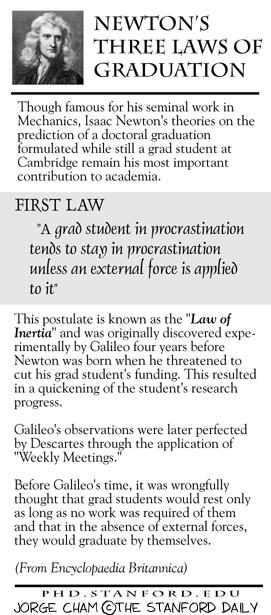
\includegraphics[width=3.5cm]{bilder/newton_1.png}
    %~ \hspace{0.55cm}
    %~ 
\includegraphics[width=3.5cm]{bilder/newton_2.png}
    %~ \hspace{0.55cm}
    %~ 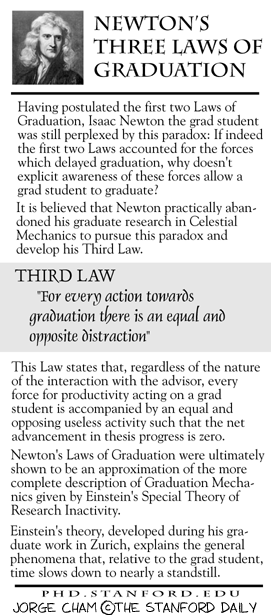
\includegraphics[width=3.5cm]{bilder/newton_3.png}
%~ }
%~ \end{figure}


%%%%%%%%%%%%%%%%%%%%%%%%%%%%%%%%%%%%%%%%%%%%%%%%%%%%%%%%%%%%%%%%%%%%%%%%%%%%
\chapter{Studieren -- wie geht das?}
\section{Lehrveranstaltungen an der Uni}
Im Gegensatz zur Schule gibt es an der Uni eine Reihe verschiedenartiger
Veranstaltungen, in denen der Lehrstoff vermittelt werden soll. Im wesentlichen
sind das: Vorlesungen, Übungen, Seminare und Praktika. Ihr habt im ersten
Semester nur mit den ersten beiden zu tun. Diejenigen unter Euch, die Physik
studieren, werden ab dem zweiten Semester auch Praktika machen. Proseminare
werden in Mathe ab dem zweiten Semester angeboten. Beides braucht Euch also
jetzt noch nicht zu beunruhigen.

Theoretisch sollte in den Vorlesungen eine Dozentin oder ein Dozent ein abgestecktes Teilgebiet der Mathematik bzw. Physik vermitteln.

Die Praxis sieht jedoch oft anders aus. In der Physik werden in atemberaubenden
Tempo erstaunliche Phänomene vorgeführt und zur Erklärung noch erstaunlichere
Formeln herangezogen, oft unterstützt durch erstaunlichste Versuche (die
mitunter zur Multi-Media-Show geraten).

In Mathe bedecken die Profs in ebenfalls atemberaubendem Tempo gleichmäßig die
Tafel mit ebenfalls erstaunlichen Zeichen die, kaum definiert, bereits in
abenteuerliche Beweise verwickelt werden.  Diese wiederum ermuntern dann einige
unterforderte Studis dazu, Quervergleiche zum Lebesgueschen Lemma und ebenfalls
verwirrenden Korollaren vorzuschlagen.

Es gibt zwei Wege, um trotz oft unbefriedigender Vorlesungspraxis an Lehrstoff
zu kommen, d.h.  etwas zu verstehen und nicht gleich am Anfang den Faden zu
verlieren. Der eine ist, Fragen zu stellen, auch wenn das häufig Überwindung
kostet. Es ist dabei gar nicht so wichtig, ob mit einer Frage etwas sofort klar
wird, es ist schon gut, dass durch eine Frage den anderen und sich selbst
Gelegenheit gegeben wird, die eigenen Gedanken zu ordnen (und nicht nur
mitschreiben zu müssen).  Außerdem wird nur so den DozentInnen gezeigt, dass es
überhaupt Fragen gibt und nicht alles selbstverständlich ist. Dabei ist zu
sagen, dass man sich mit Fragen nicht unbedingt eine Blöße gibt, denn manche
scheinbar „blöde“ Frage hat schon viele DozentInnen aus dem Konzept geworfen.

Die andere Methode folgt dem Motto: „Gemeinsam macht stark“ . Wenn ihr Euch in
Arbeitsgruppen zusammensetzt, könnt ihr Vieles klären, was Euch alleine völlig
unerklärlich schien. Für das Lösen der Übungsaufgaben (siehe unten) ist es
sowieso unerlässlich zusammenzuarbeiten, denn nur so könnt ihr damit klar
kommen.

Mit dem Wort „Übungen“ wird eigentlich zweierlei bezeichnet: Einerseits die
wöchentlich ausgegebenen Übungsaufgaben, die ihr für Eure Scheine braucht
(siehe dort), andererseits die Übungsgruppen, in denen die Aufgaben besprochen
und Probleme aus den Vorlesungen geklärt werden sollen. Auch hier gibt es
wieder Unterschiede zwischen Mathe/Informatik und Physik: In Physik werden die
Übungen in der Regel mindestens von Promovierten, oft auch von Habilitierten
(also Profs) gehalten, die jedoch der Studiertätigkeit ziemlich entwachsen
sind. Dementsprechend akademisch geht es häufig zu, viele halten eigene
Privatvorlesungen. Und auch hier gilt es, so viele Fragen wie möglich zu
stellen. Im ersten Semester werdet ihr neben dem fakultativen Basiskurs je zwei
Semesterwochenstunden Übungen in Experimentalphysik und Theoretischer Physik
haben. Manchmal werden vor Klausuren auch noch Sonderstunden angeboten, was ihr
allerdings mit Eurem Tutor ausmachen müsst.

In Mathe und Informatik werden die Übungsgruppen von Studierenden höherer
Semester, sogenannten Hiwis, gehalten. In den Übungsgruppen ist es am
leichtesten, Probleme und Verständnisfragen zu klären. Leider werden aber oft
nur die Aufgaben „heruntergerechnet“, man passt nicht mehr auf und versteht
trotzdem nicht mehr von der Aufgabe als vorher. Sollte dies der Fall sein,
fragt penetrant nach dem Sinn der Aufgabenstellung, nach ihrem Zusammenhang mit
der Vorlesung oder was Euch sonst noch durch den Kopf geht. Nur so habt ihr
eine Chance, dass ihr auch etwas aus der nervenzermürbenden Rechnerei lernt. Es
kann z.B. ein Überblick gegeben werden, wozu man einen Satz später braucht oder
auch mal ein Satz aus der Vorlesung ausführlich erklärt werden. Manchmal wird
auch zum Beginn jeder Übung die letzte Vorlesung von einem der Teilnehmer
zusammengefasst. Das gibt demjenigen die Gelegenheit, die Vorlesung intensiver
nachzubereiten, und den anderen, nochmal eine einfachere Darstellung des
Stoffes zu bekommen - und zwar von jemandem, der die gleichen Probleme wie man
selbst hat und eine andere Sichtweise als die Profs.

Natürlich ist es auch möglich, alle Veranstaltungen (bis auf die Abgabe der
scheinpflichtigen Übungsblätter) sausen zu lassen und nur aus Büchern zu
lernen. Manchmal, bei sehr schlechten Vorlesungen, ist dies sogar die einzige
sinnvolle Möglichkeit etwas zu lernen und seine Zeit sinnvoll zu nutzen. Hier
muss jedeR seinen/ihren eigenen Stil entwickeln. Sprecht Euch aber in jedem
Fall mit dem/der ÜbungsleiterIn ab, wenn ihr dort regelmäßig fehlen wollt, denn
manchmal ist die Anwesenheit und das unfreiwillige Vorrechnen notwendige
Voraussetzung für die Scheinvergabe.

\section{Vorlesungen}
\subsection{Einführung in die Praktische Informatik}
\label{info1}
Die Einführung in die Praktische Informatik (Info-I) ist für alle InformatikerInnen und Mathe-Bachelors verpflichtend. Einstieg bilden einige Grundstrukturen und Abläufe in der Informatik, die im Verlauf dann angewendet werden müssen um gegebene Probleme zu lösen. Das passiert dann meist mit einem C++-Programm, wobei aber auch das Denken in informatischen Strukturen immer mitschwingt. Idealerweise hat man am Ende genug Herangehensweisen angehäuft um Aufgaben vor dem geisten Auge zu modellieren und später in richtigen Code umsetzen zu können. Vor allem MathematikerInnen sollten die Vorlesung nicht auf die leichte Schulter nehmen, auch wenn der geringe Aufwand dazu verleitet. Spätestens mit der „Numerik 0“ muss wieder programmiert werden -- sich darum drücken kann man also nicht. Auch für LehrämtlerInnen kann es interessant sein, die Vorlesung zu hören, um sich später den Einstieg in die Numerik zu vereinfachen.

\subsection{Analysis I}
\label{ana1}

Die Analysis I (Ana I) muss von MathematikerInnen und InformatikerInnen gehört werden, jedoch sind auch PhysikerInnen nicht unbedingt schlecht beraten. Hier lernt ihr richtige, fundierte Mathematik in all ihrer Schönheit und Abstraktion (was sehr abstrakt sein kann). Diese Vorlesung hat mit dem Matheunterricht aus der Schule ähnlich viel gemeinsam wie mit dem Sportunterricht.

Ihr lernt das formell richtige Argumentieren und Beweisen und erhaltet einen Einblick darin, was das Gebäude der Mathematik eigentlich ausmacht und wie dieses aufgebaut ist. Inhaltlich beginnt sie mit der Konstruktion der reellen Zahlen, führt über Folgen und Reihen zur Stetigkeit von (reellen) Funktionen und schließlich zur Differential- und Integralrechnung. Der Arbeitsaufwand für die Vorlesung schwankt (je nach Prof) zwischen lächerlich und immens, auch hier sind zehn oder mehr Stunden für einen Zettel nicht unbedingt Seltenheit (Es lohnt sich Zettelgruppen zu bilden und gemeinsam zu rechnen). Was das unglaublich frustrierende und hilflose Gefühl betrifft, man würde nichts verstehen und wäre völlig falsch in seinem Studiengang, keine Angst, das haben alle. Wenig härtet so gut gegen Frust ab wie eine erbarmungslose Mathevorlesung im ersten Semester. Aber lasst Euch davon nicht täuschen, dass Begriffe die ihr meint aus der Schule zu kennen unnötig umständlich eingeführt werden. Es hat alles durchaus seine mathematische Berechtigung und schafft ein Fundament auf das ihr später aufbauen werdet. Sich ein sauberes, formelles Vorgehen und Denken anzugewöhnen ist unabdingbar.

\subsection{Lineare Algebra I}
\label{la1}
Die Lineare Algebra I (LA I) hören MathematikerInnen, PhysikerInnen und InformatikerInnen zusammen, bereitet Euch also auf eine sehr große Vorlesung vor. Neben den vielen Grundlagen die euch hier vermittelt werden,  handelt es sich inhaltlich um die Vektorrechnung, wie ihr sie bereits aus der Schule kennt. Diese wird jedoch viel allgemeiner und abstrakter als bisher eingeführt, was am Anfang etwas umständlich erscheint, später die Vorteile jedoch offenbar werden und „Sie sehen, dass das wieder eine Matrix wird und wir das selbe wie immer können“ (Prof. Wingberg). Im weiteren Verlauf kommen auf der Vektorrechnung aufbauend noch lineare Operatoren und Innenprodukträume hinzu, die euch Begriffe und Sätze wie Determinanten, Eigenwerte oder den Spektralsatz näher bringen. Die Inhalte werden euch euer ganzes Studium nicht mehr verlassen, da praktisch alle höheren Vorlesungen auf das mächtige Werkzeug der Linearen Algebra zurückgreifen.

\label{mathephysik}

Die Mathematikausbildung für Physiker*innen sieht vor, dass ihr die Lineare Algebra I im ersten Semester hört. Laut Modulhandbuch kann man sich dann vor dem zweiten Semester entscheiden, ob man mit Analysis II und III (was auch die Mathematiker*innen hören) oder mit Höhere Mathematik für Physiker (HöMa) II und III weitermacht.\\

Was spricht für Höhere Mathematik für Physiker (HöMa)?\\
Die Vorlesung ist extra auf euch als Physiker*innen zugeschnitten und legt ihren Schwerpunkt auf die Vorlesungen Analysis 1-3 in strafferer Form. Während Mathematikvorlesungen einer gewissen
Freiheit unterliegen und es durchaus vorkommen kann, dass die/der Dozent*in einen Schwerpunkt auf ihr/sein Forschungsgebiet legt, hört ihr in HöMa größtenteils auch nur jene Dinge, die in der Physik auch verwendet werden. Außerdem kommen Beispiele gerne aus der Physik und liegen euch deshalb vielleicht näher. Trotzdem handelt es sich nicht um eine Schmalspurversion, sondern um eine vollwertige Mathematikvorlesung, die auch für zukünftige Theoretiker nicht ungeeignet ist.\\

Was spricht für die Analysis?\\
Die Analysis bietet als eine für Mathematiker*innen konzipierte Veranstaltung eine präzisere Formulierung der Definitionen, Sätze und insbesondere Beweise. Somit wird es möglich die mathematischen Hintergründe in der Physik besser zu durchdringen und weitergehende Verbindungen der Gebiete zu erkennen. Dieses tiefere Verständnis kann unter anderem in der theoretischen Physik oder auch in weiterführenden Matheveranstaltungen von Vorteil sein und lässt euch insgesamt mehr Freiheiten im weiteren Studienverlauf, besonders bezüglich der Mathematik.
Zudem ist je nach Dozent*in und Forschungsbereich auch eine gewisse Schwerpunktlegung (vor allem in der Analysis III) möglich.\\

Auf den ersten Blick mag es verwundern, dass man in die Analysis II einsteigen soll, ohne die erste Vorlesung dazu gehört zu haben. Dies ist theoretisch zumindest möglich, jedoch vermutlich mit ein wenig Mehraufwand verbunden. Trotzdem können mathematisch Ambitionierte natürlich auch die Analysis I im ersten Semester hören, da diese eine schöne Einführung in den Themenbereich Analysis und die damit verbundenen Methoden darstellt. Das kann einem vor allem in weiterführenden Vorlesungen weiterhelfen; auch wird es eine große Erleichterung für die Analysis II sein, wenn man schon ein wenig mehr mit der Materie und dem Dozenten vertraut ist.
Andererseits werdet ihr mit dem Kursprogramm auch so schon stark ausgelastet sein. Wenn ihr es mit vier Vorlesungen versuchen wollt, solltet ihr euch nach zwei bis drei Wochen entschieden haben, ob ihr das im ersten Semester durchhaltet oder nicht, da es für den Übungsbetrieb ziemlich blöd ist, wenn in der Mitte des Semesters viele Leute aussteigen.

\subsection{Experimentalphysik I - Mechanik und Wärmelehre}
\label{ex1}

Die Physik I (Ex-I) ist eigentlich eine sehr angenehme Vorlesung, um ins erste Semester zu starten, zumindest sofern man in der Schule irgendwann mal Physik hatte. Echte Verständnishürden stellen sich gerade im Mechanikteil im Allgemeinen nicht. Im Großen und Ganzen stellt sie einen Schnelldurchlauf durch die Entwicklung der Mechanik dar, von den Anfängen (diese liegen, je nach Prof, zwischen den alten Griechen und Newtons Axiomen) bis zu etwas ausgefeilteren Sachen, die sich aber alle noch im Rahmen des Schulstoffs bewegen sollten. Was diese Vorlesung dennoch von der Schule unterscheidet ist die \emph{Art} der Präsentation, größtenteils frontaler Vortrag, gespickt mit vielen Experimenten (Manchmal durchaus eine Art „Knoff-Hoff-Show“) und sehr viel schneller und mathematischer als man das von seinem Lehrer gewohnt ist. Trotzdem ist dies die Vorlesung mit dem wahrscheinlich größten Unterhaltungswert Eurer ganzen Universitätskarriere.

\sidebar{
    \centering
    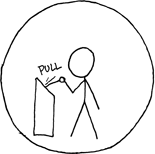
\includegraphics[width=3cm]{bilder/the_difference_1.png}\\\vspace{12mm}
    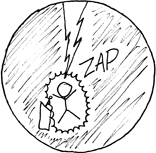
\includegraphics[width=3cm]{bilder/the_difference_2.png}\\\vspace{12mm}
    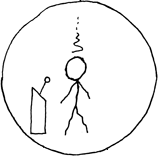
\includegraphics[width=3cm]{bilder/the_difference_3.png}\\\vspace{12mm}
    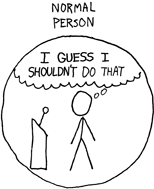
\includegraphics[width=3cm]{bilder/the_difference_4A.png}\\\vspace{12mm}
    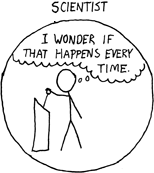
\includegraphics[width=3cm]{bilder/the_difference_4B.png}
}

\subsection{Theoretische Physik I - Mechanik und Mathem. Methoden}
\label{theo1}

Die Theoretische Physik I (Theo-I) beschäftigt sich mit der Newton'schen Mechanik und nützlichem mathematischen Werkzeug.

Hier werdet ihr im ersten Semester einige Zusammenhänge und Techniken einfach „vorgesetzt“ bekommen ohne sie völlig zu verstehen. Der genaue Grund, warum man das, was man da tut, eigentlich darf, wird im Normalfall erst in einer der späteren Mathevorlesungen klar, daran sollte man nicht verzweifeln. Dieses Vorgehen ist in der Physik nicht ungewöhnlich, was einer der Angriffspunkte von Witzen der Mathematiker über Physiker ist\dots

Ihr erhaltet hier aber nicht nur die mathematischen Techniken, die ihr in Eurem Studium brauchen werdet (und von denen ihr in vielen Fällen noch nie was gehört habt), sondern Euch wird auch eine theoretische Beschreibung der Mechanik vorgestellt. Diese unterscheidet sich im ersten Semester, bis auf einige seltsame Symbole und unglaubliche Umständlichkeit noch nicht sehr von der in der Ex-I, ab dem zweiten Semester tun sich zwischen den Sichtweisen jedoch Abgründe auf und ihr werdet verstehen, warum man auf diese Umständlichkeit bestanden hat.

Der Anspruch dieser Vorlesung an Verständnis und Wissen ist deutlich größer als in der Ex-I, womit ihr auch einen erheblich höheren Aufwand für die Bewältigung der Arbeitszettel einplanen könnt, je nach eigenem Interesse, Wissen und Perfektionismus sind zehn Stunden durchaus eine realistische Einschätzung für einen Zettel. Die Übungsgruppenleiter sind hier vor allem ältere Studierende, was den Vorteil hat, dass diese sich noch an ihre eigenen Probleme in ihrer Theo-I erinnern können und Euch das ganze verständlicher erklären können als der Theo-Prof es kann.

\section{Durchgefallen -- Was tun?}

In eurem Studium wird es aller Voraussicht nach hin und wieder vorkommen,
dass ihr durch die eine oder andere Klausur durchfallt.
Das ist an und für sich auch kein großes Problem. Zuerst einmal ist es aber
wichtig, zu wissen, was es eigentlich heißt, „durchgefallen“ zu sein.

Die meisten Leute setzen „durchgefallen“ mit „die Klausur nicht bestanden haben“
gleich. Das ist nicht ganz falsch, aber auch nicht ganz richtig. Ihr müsst
nämlich zwischen Klausur und Prüfungsleistung\footnote{ Der Unterschied zwischen
Prüfungsleistung und Prüfungsversuch besteht primär sprachlich, beide bezeichnen
meistens Klausur und Nachklausur als Einheit} unterscheiden.
In fast allen Vorlesungen werden eine Klausur und eine Nachklausur geschrieben,
die zusammen als ein Prüfungsversuch zählen. Erst wenn Ihr Klausur \emph{und}
Nachklausur nicht bestanden habt, habt ihr die entsprechende Prüfungsleistung
nicht bestanden. Ihr habt dann die Möglichkeit, die Prüfungsleistung zu
wiederholen. Dazu hört ihr das Modul dann einfach nochmal, und habt dann ein
weiteres Mal Klausur und Nachklausur vor euch. Besteht ihr beide nicht, könnt
ihr einen „Härtefallantrag“ stellen, und versuchen, vor dem Prüfungsausschuss
zu begründen, warum ihr vier Klausuren nicht bestanden habt. In der Physik habt
ihr zusätzlich in zwei Modulen einen dritten Prüfungsversuch.\footnote{Das nennt
sich dann in der Physik „Jokerregelung“} Wie genau dasgeregelt ist, steht an entsprechender Stelle im Modulhandbuch.
In der Informatik habt ihr die Chance in zusätzlich vier Modulen einen dritten Prüfungsversuch durchzuführen.

\subsection{Orientierungsprüfung}
Eine Ausnahme von dieser Regelung stellt die sogenannte \emph{Orientierungsprüfung} dar.
Diese Prüfung soll feststellen, ob Ihr überhaupt geeignet seid, das Fach, das
ihr studiert, zu studieren. Diese Prüfung müsst ihr, im Gegensatz zu allen
anderen Prüfungen, bis spätestens zum Ende des dritten Semesters erbracht haben,
und die Jokerregelung gilt hier nicht.

\subsection{Muss ich nochmal Zettel rechnen?}
Das kommt auf den Dozenten deiner Veranstaltung an. Es gibt einige, die finden,
dass man die Zettel nicht nochmal rechnen muss, einige wollen, dass du die
Zulassung noch mal neu erwirbst. So oder so ist es unglaublich hilfreich, die
Zettel trotzdem noch mal zu rechnen. Zwei mal die gleiche Veranstaltung bei zwei
verschiedenen Professoren ist eben doch ein Unterschied, und dass du
Nachholbedarf hast, hast du ja schon gezeigt ;)

\section{Was sind diese „Übungsgruppen“?}

\subsection{Übungszettel}
In den meisten Vorlesungen müsst ihr, um zur Klausur zugelassen zu werden,
Übungszettel rechnen. Das bedeutet, jede Woche werden irgendwo\footnote{Wo, wird
in der ersten Vorlesung bekannt gegeben} Übungsaufgaben hochgeladen, die ihr
euch ausdrucken und dann rechnen sollt. Weil das erfahrungsgemäß nicht so
einfach ist, und meistens viele viele Fragen auftreten, gibt es Übungsgruppen.

\subsection{Übungsgruppen}
In fast allen Vorlesungen werden vorlesungsbegleitend sogenannte „Übungsgruppen“
angeboten. Diese Übungsgruppen sind dazu da, euch bei euren Problemen mit der
Vorlesung zu helfen und die Zettel nachzubesprechen.
Dazu seid Ihr natürlich nicht auf euch allein gestellt, sondern euch wird eine
Tutorin zur Seite gestellt, die Euch bei allen Fragen, die auftreten, kompetente
Hilfe bietet.
Hier unterscheiden sich die Mathe/Informatik und die Physik: In der Physik
werden die Übungsgruppen meistens mindestens von Masterstudenten, häufig auch
von Doktoranden oder gar Profs gehalten. Dementsprechend studierendenfern sind
diese oftmals, aber natürlich gibt es auch Tutoren, die geradezu geniale
Übungsgruppen halten.
Grundsätzlich gilt es aber, so viele Fragen wie möglich zu stellen, auch um
dem Tutor Feedback zu eurem Kenntnisstand zu geben.
In der Mathe werden die Übungsgruppen in den meisten Fällen von Studierenden
höherer Semester gehalten, es ist durchaus nicht unüblich, einen Tutor zu
haben, der die Vorlesung selber erst vor zwei Semestern gehört hat.

\subsection{Was bringt mir das?}
Die Übungszettel und die dazugehörigen Übungsgruppen sind erfahrungsgemäß der
Ort, an dem euch der Stoff der Vorlesung nahe gebracht wird und ihr anfangt zu
verstehen, was eigentlich in der Vorlesung vor sich geht.
Eigentlich ist die Übungsgruppe also dazu da, die Vorlesung mit euch
nachzuarbeiten, an den Stellen an denen nicht klar ist was passiert Hilfe zu
bieten, mit euch die Zettel zu besprechen und einfach nochmal eine andere
Darstellung
Leider kommt es viel zu oft vor, dass in der Übung nur die Aufgaben
„runtergerechnet“ werden, man irgendwann nicht mehr aufpasst und am Ende auch
nicht mehr weiß, als vorher.  Wenn das passiert, fragt penetrant nach dem Sinn
der Aufgabenstellung, nach dem Zusammenhang mit der Vorlesung oder nach was
euch sonst noch so durch den Kopf geht. Das ist eure einzige Chance, noch etwas
aus der Rechnerei zu lernen.

\subsection{Anmeldung}
Ganz häufig stellen sich anfangende Studierende die Frage, ob sie sich zu den
Übungen anmelden müssen. Die Antwort ist meistens „ja“.
In der Physik nutzt man dazu das physikinterne Übungsgruppensystem\footnote{\url{https://uebungen.physik.uni-heidelberg.de/uebungen/}}
Das System ist leider nicht besonders leistungsfähig. Da kann es schon mal
vorkommen, dass es zu Zeiten, in denen die Übungsgruppenanmeldung großer
Vorlesungen freigeschaltet werden, abkackt. Das ist aber auch kein Drama, und
insbesondere kein Grund, das Rektorat zu alarmieren\footnote{Wann das wohl
passiert ist…}, denn nach einigen Minuten hat sich das System dann auch wieder
gefangen.
Die Mathe geht wie immer ihren eigenen Weg, und hat mit dem Müsli\footnote{Mathematisches Übungsgruppen- und ScheinListenInterface:\\ \url{https://www.mathi.uni-heidelberg.de/muesli/}}
Das ist deutlich leistungsfähiger, deutlich besser und viel schöner, aber man
kann als Physiker ja nicht alles haben.
Die Informatik wiederum nutzt in 90\% aller Fälle das Moodle\footnote{\url{https://elearning2.uni-heidelberg.de/}}, das E-Learning-System der Uni Heidelberg.
90\% aller Nutzer sind sich einig, dass dieses System ganz doll Grütze ist, aber
davon hat sich die Informatik noch nie beeinflussen lassen.

\section{Praktika}

In der Physik werdet ihr früher oder später Praktika absolvieren.
Dabei geht es darum, dass ihr eure ganzen erworbenen Kenntnisse aus den
Ex-Vorlesungen endlich anwendet, um eigene „Forschung“ zu betreiben.

\subsection{Wann ist das?}
In den Semesterferien zwischen dem zweiten und dem dritten Semester geht der
Praktikums-Spaß mit dem AP 1\footnote{AP == AnfängerPraktikum} los.
In eurem dritten Semester, den Semesterferien zwischen drittem und viertem
Semester und im vierten Semester absolviert ihr die beiden Teile des AP 2.
Ihr könnt euch dabei selber einteilen, welchen Teil ihr wann macht.
Erfahrungsgemäß ist AP 2.1 etwas mehr und etwas komplizierter, daher ist es
empfehlenswert, diesen Teil in den Semesterferien zu machen.

Sobald ihr eure Anfängerpraktika hinter euch habt, dürft ihr mit dem FP
\footnote{FP == FortgeschrittenenPraktikum} anfangen. Auch hier gibt es wieder
zwei Teile und ihr müsst aus beiden Teilen mindestens 3 Versuche machen,
insgesamt stehen 8 Versuche auf dem Plan. Zu einem davon müsst ihr dann auch
noch einen Vortrag halten, und zu einem müsst ihr eine ganz besonders
ausführliche Auswertung schreiben. Das FP wird aber nicht mehr -- wie die AP --
als Blockveranstaltung angeboten, sondern ihr dürft euch eure Versuche selber
so legen, wie es euch gerade passt -- vorrausgesetzt der Versuch wird dann, wann
ihr wollt, angeboten.

\subsection{Und wie geht das?}
Das grundlegende Konzept der Praktika ist, dass ihr selber einige Ergebnisse
aus Ex 1-5 reproduziert. Sei es jetzt die Erdbeschleunigung über
Pendelschwingungen oder die Boltzmannkonstante aus Brown'scher Bewegung, ihr
messt selber, wertet eure Ergebnisse selber aus und müsst selbst bewerten, ob
das, was ihr gemacht habt, signifikant ist.

Dabei gehen fast alle Versuche nach dem gleichen Schema vor:
Ihr bekommt ein Skript, in dem die Theorie des Versuchs, die Durchführung und
die Auswertung ausführlich beschrieben sind. Ihr schreibt dann mithilfe dieses
Skripts eine Einleitung zu eurem Versuch, in der ihr in eigenen Worten
formuliert, was ihr eigentlich tun werdet.
Am Tag des Versuchs selber werdet ihr von eurem Betreuer dann abgefragt, ob ihr
Bescheid wisst, was zu tun ist. Danach messt ihr alle wichtigen Größen für
diesen Versuch selber an den entsprechenden Apparaturen.
Ist das geschehen, schreibt ihr eine Auswertung, in der ihr die gemessenen
Größen auswertet und das eigentliche Resultat produziert.

\section{Seminare}

In eurem Studium werdet ihr früher oder später über Seminare und Proseminare
stolpern, in der Mathe früher und mehr als in der Physik.
Seminare dienen dazu, dass ihr euch selber ein Thema erarbeitet und dann lernt,
das vorzustellen.

Seminare fangen immer mit der Seminarvorbesprechung an. Alle Leute, die an dem
Thema interessiert sind, treffen sich und der Seminarbetreuer stellt die Themen
der einzelnen Vorträge vor und danach werden sie an die Teilnehmer vergeben.
Die Seminarvorbesprechungen in der Mathe finden meistens in der letzten Woche
des alten Semester statt, in der Info und Physik in der ersten Woche des neuen
Semesters.

Sobald ihr also euer Thema habt, habt ihr (je nach Thema) zwei Wochen bis ein
Semester Zeit, um euch vorzubereiten. Ihr lest also das entsprechende Kapitel
in dem Buch nach dem das Seminar gehalten wird oder beschäftigt euch sonst
mit dem Thema. Im Unterschied zu Vorlesungen arbeitet ihr euch selber in das
Thema ein, müsst euch Beweise oder Zusammenhänge selber überlegen und seid dann
selbst gefordert, denn ihr müsst das zuvor gelernte selber an die Tafel bringen.

Falls ihr irgendwo in eurer Vorbereitung über Dinge stolpert, die ihr nicht
versteht, oder falls irgendwo Fragen auftauchen, die ihr selber nicht
beantwortet bekommt, könnt ihr euren Seminarbetreuuer fragen, denn genau das
ist sein Job.

\subsection{Proseminar oder Seminar?}
Für viele Leute ist ein Seminar das erste Mal, dass sie an der Tafel stehen.
Weil in Seminaren der Inhalt doch stark im Vordergrund steht, gibt es in der
Mathe zusätzlich zu Seminaren auch noch sogenannte Proseminare. Der Unterschied
ist der folgende:
Seminare sind dazu da, euch ein bestimmtes Thema, das für eine Vorlesung zu
speziell wäre und zu wenig Leute interessiert, nahe zu bringen.
Diese Themen sind meistens relativ komplex und ihr müsst euch selber mit dem
Inhalt beschäftigen, selber Gedanken machen und quasi selber „Mathe“
produzieren. Der Fokus liegt also klar auf der Mathe und wenig auf eurem
Vortrag.
In Proseminaren hingegen sollte der Fokus auf dem Vortrag, und weniger auf dem
Inhalt liegen. Der ist natürlich auch wichtig, und man sollte nicht erwarten,
dass ein Proseminar inhaltlich einfach wird, aber meistens sind auch schwere
Prosenimare weniger anspruchsvoll als leichte Seminare.
Nach eurem Vortrag wird dieser daher deutlich ausführlicher analysiert und
nachbesprochen, als es bei einem Seminar der Fall wäre.

\subsection{Und wozu mache ich das?}
Für ein Seminar gibt es drei Gründe.

Der erste, und wohl offensichtlichste ist, dass es im Bachelor Pflicht ist.

Der zweite und wohl ebenso offensichtliche ist, dass Seminare die Möglichkeit
bieten, Themengebiete kennen zu lernen, die in den Grundvorlesungen nicht
vorkommen oder nur angeschnitten werden, oder sich in bestimmten Bereichen zu
vertiefen.

Der dritte und nicht ganz so offensichtliche Grundist, dass die meisten Profs
Seminare nutzen um die Studierenden kennenzulernen, die bei ihnen
Bachelorarbeiten schreiben wollen.  In der reinen Mathe geht das sogar so weit,
dass es relativ unmöglich ist, eine Bachelorarbeit zu bekommen, ohne vorher ein
Seminar gehört zu haben.  Die angewandte Mathe sieht das nicht ganz so eng,
aber auch da ist ein Seminar oder eine Vorlesung beim entsprechenden Prof
empfehlenswert.  In der Physik haben Seminare keinen so großen Stellenwert wie
in der Mathe, in den meisten Fällen hören Bachelorstudenten genau eines -- ihr
Pflichtseminar.

\section{Lehrbücher}

Bücher sind in erster Linie eine Geschmackssache. Die meisten Bücher, die
hier aufgelistet werden, behandeln Elemente des Stoffes, der für die ersten
zwei Semester gebraucht wird. Das richtige Buch für sich selbst zu finden,
geht aber nur durch Ausprobieren! Jedem Lerntyp liegen unterschiedliche
Herangehensweisen und damit auch unterschiedliche Bücher. Hier für sich
selbst den richtigen Weg zu finden, kann durchaus seine Zeit dauern -- macht
euch deshalb nicht verrückt wegen der Büchersuche, die Physik und Mathe ist
letztendlich in allen Werken die Gleiche.

Es ist jedoch durchaus empfehlenswert, in einer ruhigen Minute mal ein Thema
in verschiedenen Büchern nachzulesen. Dabei lernt man nicht nur viel über die
eigene bevorzugte Herangehensweise, die unterschiedlichen Blickwinkel können
auch dazu beitragen, ein Thema umfassender (oder überhaupt erst) zu verstehen.

Neben der Möglichkeit, sich in der Universitätsbibliothek Bücher auszuleihen,
darf hier auch ein Hinweis auf den Lesesaal nicht fehlen: Im Erdgeschoss der UB
befindet sich ein großer Bereich mit Arbeitsplätzen, in dem ein großer Teil der
Lehrbücher als Ansichtsexemplare ausliegen.  Dort kann man sich die
verschiedenen Bücher in Ruhe genauer ansehen, außerdem wird dieser Bereich von
manchen Studierenden auch als Lernumgebung sehr geschätzt, da dort absolute
Ruhe und eine sehr konzentrierte Lernatmosphäre herrscht und man alle nötigen
und unnötigen Nachschlagewerke direkt vor Ort hat. Ähnliches gilt übrigens auch
für die Präsenzbibliotheken der Fakultäten (s.o.).

Falls ihr vorhabt, ein Buch zu kaufen, dann lasst Euch Zeit dafür und leiht euch
die Bücher lieber erst einmal aus (alle hier vorgestellten Bücher sind im Bestand
der Leihbibliothek). Beim ersten Durchblättern eines Buches kann man meistens
nicht feststellen, ob einem die Art und Weise der Stoffvermittlung liegt. Das
führt häufig im ersten Semester dazu, dass in Extremfällen kleine dreistellige
Beträge für Fachliteratur ausgegeben werden, die anfangs als absolut notwendig
erscheint und sich dann nach einiger Zeit doch als mehr oder weniger nutzlos
erweist, weil einem die spezielle Herangehensweise des Buches zufällig nicht liegt\dots

Für viele Vorlesungen haben die Dozierenden ein Skript erstellt, was häufig eine gute
Hilfe bei der Nachbereitung des Stoffes ist. Einige dieser Skripte werden auch gedruckt
und im Laufe des Semesters in den Vorlesungen ausgeteilt. Anschließend sind sie im 
Fachschaftsraum kostenlos erhältlich -- kommt einfach bei uns vorbei und fragt nach,
ob das auch bei euren Vorlesungen der Fall ist.

Weiterhin solltet ihr auf jeden Fall die Skriptensammlung\footnote{\url{http://mathphys.fsk.uni-heidelberg.de/w/hauptseite/skripte/}}
der Fachschaft im Netz durchstöbern. Unter „Skriptensammlung (PDFs)“ findet
ihr unsere Links zu Vorlesungsskripten (dort finden sich passende Skripte zu fast
jeder Vorlesung).

\subsubsection{Analysis}
\begin{description}
%\item[Barner/Flohr: Analysis~I,~II; deGruyter]
%{Dieses zweibändige Werk führt ausführlich in das Gebiet der
%Analysis ein und ist zum Lernen des Stoffs gut, zur
%Prüfungsvorbereitung allerdings nur bedingt geeignet.}

\item[Forster] {Die ersten zwei
Bände behandeln recht knapp und kompakt den Stoff der ersten
zwei Semester des Analysis-Kurses. Der dritte Band ist ebenfalls
knapp geschrieben, allerdings sehr umfangreich, so dass meist
nicht einmal die Hälfte des Buches im dritten Semester behandelt
werden kann. Ein Standardbuch, da es auch sehr preisgünstig ist.
Aber zum erstmaligen Lernen nur bedingt geeignet,
dagegen zur Prüfungsvorbereitung relativ gut geeignet (Viele
Übungsaufgaben mit Lösungen in einem Extra-Band).}

%\item[Heuser: Lehrbuch der Analysis~I,~II; Teubner]{
%Sehr umfangreich mit vielen Beispielen und "Ubungsaufgaben (zum Teil mit
%Lösungen), dafür artet die Beschreibung streckenweise in Laberei aus.
%Das Buch enthält dafür allerdings viele historische Bemerkungen, die
%sehr interessante Einblicke in den Stoff und die Entwicklung der
%entsprechenden Themengebiete ermöglichen. Damit ist es zur
%Prüfungsvorbereitung nicht so gut  geeignet -- höchstens für
%Verständnisprobleme. Der hohe Umfang schlägt sich leider auch im
%Preis nieder.}

\item[Königsberger]{
Ein gut strukturiertes Standardbuch. Es wird nicht nur der Stoff der
ersten beiden Semester behandelt, sondern darüber hinaus auch einige
damit zusammenhängende oder weiterführende Themen. Es ist
deutlich ausführlicher geschrieben als Forster und ist so nicht nur
hervorragend zur Prüfungsvorbereitung geeignet, sondern auch
begleitend zur Vorlesung.}

%\item[Walter: Analysis~I,~II; Springer]{
%Ein Buch, das sich sehr gut liest und in etwa in der Mitte zwischen
%Forster und Heuser liegt. Für diejenigen, die mit dieser Art der
%Wissensübermittlung zurechtkommen, ist dies ein „Buch für
%alle Fälle\grqq.}

%\item[Behrens: Analysis ~I, ~II; Vieweg]{
%Mit studentischer Hilfe geschrieben. Wem andere Bücher zu kompliziert
%und unverständlich sind, hat hier oft an der richtigen Stelle die
%richtige Erklärung. Geht allerdings nicht so in die Tiefe, wie
%Königsberger oder Amann, Escher.}

\item[Amann, Escher]{
Ein sehr umfangreiches Buch, welches extrem in die Tiefe geht und eine
schöne Querverbindung zur linearen Algebra schlägt. Wer dieses Buch
durchgearbeitet bekommt, hat wohl alles Wissenswerte gut genug verstanden.
Allerdings ist es ziemlich kompliziert und damit für die meisten Studis 
als erstes Buch nicht geeignet.}

%\item[Weiterführende Werke]{ sind von vielen Autoren erhältlich, hier seien
%nur Dieudonn\'e und S.~Lang erwähnt. Diese Bücher eignen sich aber
%nur zum Vertiefen von schon vorhandenen Analysiskenntnissen und nicht
%zum Studienbeginn.}
\end{description}


\subsubsection*{Lineare Algebra}
\begin{description}
\item[Fischer]{
Ein Standardwerk, das durch seinen günstigen Preis und seine kompakte
Darstellung zum wohl meistgelesenen LA-Buch geworden ist. Es ist
empfehlenswert, wenn man sich nicht von der etwas abstrakten Darstellung
abschrecken lässt. Es bringt den vollständigen Stoff der ersten zwei
Semester in einem Band (natürlich profabhängig). Zur
Prüfungsvorbereitung
ist es relativ gut geeignet. Wem die Mathematik zum Studienbeginn
sowieso
schon zu abstrakt ist, dem sei eher der Beutelspacher empfohlen.
Man sollte die älteren Auflagen (alles vor 10.) meiden, da sie
unübersichtlich sind.}

%\item[Anton: Lineare Algebra; Spektrum]{
%Gut geeignet für alle Studis, die zur oft trockenen Theorie der
%Vorlesung
%viele, viele Beispiele brauchen. Sehr leicht verständlich, umfasst er
%dennoch fast den gesamten Stoff aus LA 1 bis hin zur
%Hauptachsentransformation.}

%\item[Jänich: Lineare Algebra; Springer]{
%Dieses Buch ist wohl die einfachste Hinführung zu den ersten
%Begriffen der LA.
%Allerdings hat es den sehr großen Nachteil, dass in dem Buch nicht
%einmal
%der Stoff der ersten $\frac{2}{3}$ des ersten Semesters behandelt wird. Ein
%Buch, das
%Ihr Euch ausleihen solltet, aber zum Kauf eher nicht geeignet ist. Zur
%Prüfungsvorbereitung ist es absolut ungeeignet.}

%\item[Lipschutz: Lineare Algebra; Schaum's Outline]{
%Dieses Buch ist nicht als Lehrbuch konzipiert, sondern im wesentlichen
%zur
%Prüfungsvorbereitung gedacht, also wenn man einen Haufen
%Beispielaufgaben
%durchrechnen will. Zur Theorievermittlung ist es nicht geeignet.}

%\item[Lorenz: Lineare Algebra I, II; BI-Verlag]{
%Eine etwas theoretischere Einführung in die LA, die vor allem auch
%schon
%Begriffe aus der Algebra übermittelt. Besonders geeignet ist dieses
%Buch für
%Studierende, die sich später in Richtung reine Mathematik
%spezialisieren
%wollen. Aber auch alle anderen, die sich mit dieser Art der
%Präsentation des
%Stoffes zurechtfinden, ist dies ein empfehlenswertes Buch zum
%erstmaligen
%Lernen und zur Prüfungsvorbereitung. Der Stoff\-umfang des Buches geht
%etwas über den in den ersten zwei Semestern vermittelten Stoff
%hinaus.}

\item[Beutelspacher]{
Die wohl zugänglichste Einführung in die Lineare Algebra. Der Autor
verzichtet weitestgehend auf Formeln und versucht, die Ideen möglichst
intuitiv und sprachlich zu vermitteln. Daher ist es für Studis, denen
die
mathematische Vorgehensweise im Studium zu abstrakt ist, sehr zu
empfehlen.
Problematisch ist allerdings, dass gerade diese Fähigkeit zum
Abstrahieren eines der wichtigsten Ziele des ersten Semesters ist.
Außerdem ist der Stoffumfang nicht sehr
groß, wer also mal die ersten Hürden der Mathematik überwunden hat,
sollte
das Buch wechseln.}

%\item[Koecher: Lineare Algebra und analytische Geometrie; Springer]{
%Dieses Buch bringt den Stoff von zwei Semestern zusammen mit Einigem an
%analytischer Geometrie, aufgelockert mit historischen Bemerkungen und
%sehr gut
%gegliedert, allerdings auch ein wenig theoretischer als das Buch von
%Fischer.
%Für die Einführung ist das Buch nur mäßig geeignet, da es manches
%an
%Vorwissen fordert und Beweise teilweise sehr kurz abgehandelt werden.}

%\item[Kowalsky: Lineare Algebra; deGruyter]{
%Ein gutes Lehrbuch, das ähnlich wie der Fischer eher abstrakt
%geschrieben
%ist, aber dennoch verständlich (und nicht zu kurz) erklärt. Der
%behandelte
%Stoff ist mal abgesehen vom Brieskorn am unfangreichsten. Sowohl
%zum Lernen als auch zum Nachschlagen zu empfehlen.}

%\item[Walter: Einführung i. d. LA und analytische Geometrie; Vieweg]{
%Ein sehr gut aufgebautes Buch, das allerdings viel mehr als den
%üblichen Stoff
%%(in den ersten zwei Bänden) vermittelt. Dieses Buch ist zwar teuer
%für ein Grundvorlesungsbuch, doch didaktisch gut aufgebaut und sowohl
%zum Lernen
%als auch zur Prüfungsvorbereitung sehr gut geeignet.}

%\item[Brieskorn: Lineare Algebra und analytische Geometrie ~I,~II;
%Vieweg]{
%Die Bibel der LA. Hier steht (fast) alles drin, was zur Folge hat,
%daß das
%Lesen dieses Buches schnell zur Qual werden kann. Als Nachschlagewerk
%nur bedingt geeignet. Die Anschaffung dieses Buches lohnt sich
%wirklich nur
%für die, die sich mehr mit LA beschäftigen wollen.}

%\item[Bröcker: Lineare Algebra und analytische Geometrie; Birkhäuser]{
%Wenn man Frau Böge glaubt, DAS Buch für eine Prüfung in linearer
%Algebra. Der Stoffumfang ist groß doch
%muss man leider vorne anfangen zu lesen, der Umstieg von anderen
%Büchern auf den Bröcker wird einem nicht
%immer leicht gemacht. Er behandelt einiges, was nicht in jeder
%LA-Vorlesung dran kommt, liest sich dennoch
%ganz angenehm, wenn man sich die Zeit nimmt mit ihm zu arbeiten.}

\item[Bosch]{
Ein gutes Lehrbuch, welches in Heidelberg oft begleitend zur Vorlesung
verwendet wird. Es führt zuweilen relativ abstrakt in die Lineare
Algebra ein und legt bereits dort Grundlagen für die weitergehenden
Algebra-Vorlesungen, die man in anderen LA-Büchern nur zum Teil findet.
}

%\item[dtv Atlas für Mathematik]{
%Handliches und sehr preiswertes Nachschlagewerk. Aufgelistete
%Stichworte werden kurz und verständlich beschrieben und teilweise mit
%bunten Bildern erklärt. Sehr zu empfehlen.}
\end{description}

\subsubsection{Experimentalphysik}
\begin{description}

%\item[Alonso/Finn: Physik; Addison-Wesley]{
%Ein Komplettwerk der Experimentalphysik für die ersten zwei Semester.
%Die
%Darstellung der Physik ist ein wenig mathematischer als üblich, aber
%trotzdem
%ist es ein sehr empfehlenswertes Buch.}

%\item[Bergmann/Schäfer; deGruyter]{
%%Hier steht alles drin, was Mensch über Experimentalphysik wissen muß
%und noch
%viel, viel mehr. Diese Reihe ist nur zum Nachschlagen geeignet, denn
%alles zu
%lernen, was in ihr steht, ist unmöglich. Trotzdem sind diese Bücher
%gut
%geschrieben und eignen sich auch zum Lernen, es muß allerdings stark
%ausgewählt werden.}

%\item[Berkeley Physikkurs; Vieweg]{
%Ein insgesamt sechsbändiger Kurs, dessen erste drei Bände für die
%ersten
%zwei Semester bei weitem ausreichen. Die Reihe ist, ähnlich wie der
%Alonso/Finn, etwas theoretischer gehalten als die deutschen Lehrbücher
%(Gerthsen, Bergmann/Schäfer, ...) und geht an vielen Stellen deutlich
%tiefer,
%als es für das erste Lesen notwendig ist. Diese Stellen können aber
%auch
%guten Gewissens erst einmal überblättert werden und sind später zum
%Verständnis sehr wertvoll. Liest sich ansonsten sehr schön und hat
%auch
%mal bessere Erklärungen, als die deutschen Bücher.}

\item[Demtröder]{
Ein insgesamt vierbändiges Werk. Die Erklärungen sind gut und
tiefgehend, dafür ist das Buch stellenweise sehr theoretisch. Beim
ersten
Lesen empfiehlt es sich, einige Paragraphen zu überspringen. Zum Lernen
und zur Prüfungsvorbereitung ist es sehr empfehlenswert, doch muss
man bei
speziellen Themen und komplizierteren Formeln aufpassen, da selbst die
dritte
Auflage noch stark von Fehlern durchsetzt ist. Inzwischen hat sich das
Buch
trotzdem zu einer Art Standardwerk entwickelt, besonders in den höheren
Experimentalphysikvorlesungen eignet sich das Buch bei vielen Profs
sehr gut
für die Vorlesungsnachbereitung.}

\item[Feynman]{
Diese Bücher sind wunderschön zu lesen, da sie weniger aus Formeln,
sondern
hauptsächlich aus Erklärungen bestehen. Manche finden sie einfach
genial,
andere halten es nur für Gelaber. Es ist aber das einzige Buch, das
wirklich versucht,
Verständnis zu vermitteln (und nicht nur Wissen). Zum Nachschlagen
ist dieses Buch
denkbar ungeeignet -- für die verzweifelten Studierenden, die gerade dabei
sind, den Spaß
am Studium zu verlieren finden sich hier aber zahlreiche Passagen, die
sehr anschaulich
und auf eine unnachahmliche Art und Weise Physik vermitteln und so die
Freude am
Studium wiederbeleben können.}

%\item[Vogel: Gerthsen Physik; Springer]{
%Das Standardwerk schlechthin. Hier steht so ziemlich alles drin,
%was Mensch wissen muß. Die Meinungen sind allerdings auch hier geteilt.
%Die Erklärungen sind meist zu knapp, um Verständnis zu übermitteln
%und
%manche kommen mit dem Stil des Buches nicht zurecht. Dafür ist
%es locker geschrieben, geht sehr in die Tiefe und enthält interessante
%Aufgaben.}

\item[Tipler]{
Das Buch enthält den Stoff der ersten drei Semester. Die Erklärungen
sind
sehr ausführlich, das Buch eignet sich daher hervorragendend zum
Lernen und
zur Prüfungsvorbereitung. Es wird viel Wert auf Verständnis und
Aufgaben
gelegt und es ist einfach nett, im Tipler zu lesen. Allerdings werden
die
Themen nicht immer in der nötigen Tiefe behandelt. Es ist ein
Buch zum Lernen, nicht zum Nachschlagen. Super ist der Aufgabenteil,
zu dem es
ein Lösungsheft mit ausführlichen Beschreibungen gibt. (Den Tipler
könnt ihr euch auch
im FS-Raum ansehen.)}

%\item[dtv Atlas für Physik]{
%Handliches und sehr preiswertes Nachschlagewerk. Aufgelistete
%Stichworte werden
%kurz und verständlich beschrieben und teilweise mit bunten Bildern
%erklärt. Sehr zu empfehlen.}
\end{description}

\subsubsection*{Theoretische Physik}

Bei Büchern der theoretischen Physik muss man leider immer damit rechnen,
dass sie einen recht abstrakten Blick auf die Welt haben didaktisch nicht
dermaßen hervorragend sind, wie man sich das oft wünscht. 

\begin{description}

%\item[Goldstein]{
%Wohl das erste richtige Mechanik Buch, deshalb auch nicht mehr auf der
%Höhe der Zeit,
%was Didaktik und Methodik angeht. Trotzdem wird von Profs und Autoren
%gerne mal auf ihn
%zurück gegriffen.}

%\item[Kuypers]{
%Klassiker unter den Theo I Büchern. Behandelt wohl alles was man in
%der Mechanik machen
%kann und hat genügend ‹bungsaufgaben mit Lösungen.}

\item[Fließbach]{
Eines der einfacheren Bücher, allerdings auch nicht so umfangreich
und auch nur bedingt für das erste Semester geeignet, da die Newton'sche Mechanik
nur sehr knapp behandelt wird. Wer mit der theoretischen Physik 
Schwierigkeiten hat, findet hier ab dem zweiten Semester ein gutes Buch.
Dazu passend gibt auch ein Arbeitsbuch, in dem alles noch mal zusammengefasst
und an Aufgaben erläutert wird. (Beide sind im FS-Raum einzusehen.)}

%\item[Greiner]{
%Ein Buch, was für Leute wie Euch geschrieben ist, da in Frankfurt
%schon länger im ersten
%Semester mit der Theo I angefangen wird. Auch sonst ein hat das Buch
%Hand und Fuß.}

\item[Nolting]{Mehrbändige Theo-Reihe, die vor allem beim Lösen von
Übungsaufgaben und bei der Klausurvorbereitung hilfreich ist. Sehr
gut und nachvollziehbar strukturiert und eignet sich deshalb auch
zum Wiederholen. Entspricht bis auf die Reihenfolge von der
Vorgehensweise auch den Heidelberger Theorievorlesungen.
}

\item[Bartelmann]{Diese Komposition aus Heidelberger Gefilden deckt
alle für das Studium relevanten Bereiche der Theoretischen Physik in
einem Band ab. Geschrieben von Koryphäen der Lehre wird das Buch von
vielen Studierenden als sehr gut empfunden.}

%\item[Scheck]{Etwas komplizierter und anspruchsvoller als andere
%-- wer mal ein streng mathematisch geschriebenes Buch haben will,
%kann hier mal rein schauen. Behandelt viele Themen unter einem
%konzeptuell breiteren Aspekt als typische Theo-Bücher. Der
%Klassiker in dieser Hinsicht ist allerdings immer noch der
%Landau/Lifschitz. Dennoch in höheren Semestern lesenswert.}

%\item[Landau, Lifschitz]{
%Wohl das höchste der Gefühle, wenn es nach manchen Theoretikern geht.
%Für die Vorlesungen aber in der
%Regel zu abgefahren.}
\end{description}


\subsubsection{Mathematische Methoden}

Eine Vorlesung, die ihr zwar nicht mehr hört, doch trotzdem sind die
Themen für
Physiker wichtig, da hier die Mathematik auf Gebrauchsniveau gehievt
wird.

\begin{description}

\item[Boas: Mathematical Methods in the Physical Science]{
In diesem Buch wird die Mathematik so gebracht, wie sie in der Physik
gebraucht
wird. Es ist wohl das beste Buch zu diesem Thema. In der Boas werden
zahlreiche
für Physiker wichtige Vorgehensweisen anschaulich erklärt und in
vielen
Beispielen ausführlich vorgerechnet. Außerdem enthält das
Buch Aufgaben mit Lösungen. Vor dem Englisch braucht ihr keine Angst zu
haben, denn mathematical english ist immer sehr viel einfacher als
normal
english. Sehr zu empfehlen, sowohl als Nachschlagewerk als auch um
verschiedene
generelle Schwierigkeiten zu beheben.}

\item[Lang, Pucker: Mathematische Methoden in der Physik]{
Dieses Buch wird zur Zeit von den DozentInnen empfohlen und ist in etwa
äquivalent zur Boas -- nur auf Deutsch und etwas günstiger in der
Anschaffung.
Teilweise etwas weniger ausführlich.}

%\item[Großmann: Mathematischer Einführungskurs i. d. Physik]{
%Behandelt den Stoff des Vorkurses und etwas mehr. Es ist
%wahrscheinlich besser,
%gleich ein weiterführenderes Werk zu erwerben, ansonsten aber gut zum
%Einsteigen.}

%\item[Hefft: Mathematischer Vorkurs zum Studium der Physik]{
%DAS Begleitbuch zu eurem Vorkurs, später wohl weniger nützlich.
%Glaubt nicht,
%dass ihr alles verstehen müsst, was euch da serviert wird -- es ist
%aber schön, von den
%ein oder anderen Dingen schonmal etwas gehört zu haben.}

\item[Otto: Rechenmethoden für Studierende der Physik im ersten Jahr]{
In diesem Buch ist die Mathe, die man in den ersten beiden Semestern eines Physikstudiums braucht, anschaulich und ausführlich erklärt. Dabei wird bewusst auf mathematische Beweise verzichtet und mehr auf die physikalische Interpretation eingegangen. Sehr gut geeignet für Studies, die sich am Anfang in Theo ein wenig von der Mathe überrumpelt fühlen.}
\end{description}

\subsubsection*{Nachschlagewerke}

Als eine kommentierte Formelsammlung können folgende Bücher dienen:

\begin{description}

\item[Bronstein/Semendjajew]{
Eines der Bücher, die man als Physiker von jedem Prof empfohlen
bekommt -- zu
Recht. Da das Buch nur die Formeln und Beispiele enthält und keine
Beweise,
ist es für Mathematiker nicht so interessant, trotzdem aber nützlich,
wenn
man irgendetwas berechnen muss. Der Bronstein hat sich bei"
PhysikerInnen
zu einer Art Bibel entwickelt (jeder hat es, jeder benutzt es) da
hierin jede Menge Integrale,
Taylorreihenentwicklungen, usw. aufgelistet werden.}

\item[Stöcker: Taschenbuch der Physik]{
Experimentell orientiertes, sehr kompaktes Nachschlagewerk mit
teilweise sehr
guten und einprägsamen Erklärungen für die stabile Studi-
Jackentasche.
Auch praktisch zum Lernen in Bus und Straßenbahn.}
\end{description}


%%%%%%%%%%%%%%%%%%%%%%%%%%%%%%%%%%%%%%%%%%%%%%%%%%%%%%%%%%%%%%%%%%%%%%%%%%%%%
\chapter{An der Uni \dots}
\section{Kummerkasten}
\label{kummerkasten}

Dank des KummerKasten\footnote{\url{http://kummerkasten.uni-hd.de}} kannst du den Dozentinnen und Dozenten einfach und anonym eine Nachricht
zukommen lassen, und so bereits während der Vorlesung Rückmeldung geben. Dabei
kann es sich um technische Probleme (Mikrofonanlage zu leise), inhaltliche
Aspekte (Vorlesungstempo zu gering) aber selbstverständlich auch Lob handeln.
Alles was nicht die DozentInnen direkt betrifft, was sie nicht beantworten
können oder beleidigend ist, wird dabei durch die Fachschaft zurückgehalten.
Inhaltliche Fragen solltet ihr an eure Tutorin oder euren Tutor richten; gibt
es Probleme mit dem Übungsbetrieb wendet euch an die Obertutorin bzw. den
Obertutor. Im Zweifelsfall kannst Du der Fachschaft eine
E-Mail\footnote{\email{fachschaft@mathphys.fsk.uni-heidelberg.de}} schreiben,
da auch wir dir über den KummerKasten nicht antworten können.

% !TEX ROOT = ../ersti.tex
\section{EDV}

\subsection{Universitätsrechenzentrum (URZ)}
\label{urz}
Computer sind die Triebfeder unseres Zeitalters und auch im Studium kommt ihr nicht um sie herum. Das beginnt zum Beispiel schon damit, dass die meisten Übungszettel nur online erscheinen und selbst ausgedruckt werden müssen. Später möchtet ihr eure Bachelor- oder Masterarbeit bzw.\ eure Examensarbeit sicher nicht handschriftlich anfertigen sondern lieber in \LaTeX \footnote{„Latech“ gesprochen. LibreOffice -- oder noch schlimmer -- Word helfen nicht weiter, weil man Formeln nur sehr umständlich eingeben kann. Außerdem schafft es \LaTeX{} Blocktexte ohne größere Freiräume und mit weniger Bindestrichen zu setzen, wie man z.\,B.\ an diesem Ersti-Info sehen kann. Wenn ihr \LaTeX{} lernen möchtet, haltet in den nächsten Semestern nach einem entsprechenden Kurs Ausschau oder nutzt eins der vielen Onlinetutorials.} setzen. Das  \gls{URZ} bietet eine ganze Menge von Services an, die hier kurz erläutert werden sollen.

\subsection*{Multifunktionaler Studierendenausweis (Campus Card)}
\label{campuscard}
Wie an den meisten Unis ist der Studierendenausweis auch in Heidelberg voll modern und also multifunktional.
Neben der Ausweisfunktion wird er zum Ausleihen von Büchern in der Universitätsbibliothek und als „Geldkarte“ zum Bezahlen sowohl in der Mensa als auch an Kopierern und an einigen Waschstationen des Studentenwerks benutzt. Um diese Funktion nutzen zu können, muss man Geld auf den Ausweis laden, dafür stehen in den Mensen Automaten zur Verfügung.
Zusätzlich gilt der Ausweis im \gls{VRN} werktags ab 19 Uhr und an Wochenenden ohne Zeitbegrenzung auch als Fahrausweis (siehe auch \autopageref{verkehrsmittel}).

Auf dem RFID-Chip der Karte ist nur die ID für die Bezahlfunktion des Studentenwerks gespeichert und daher auch die einzige Information, die sich ohne Sichtverbindung auslesen lässt. Sofern euer Geldbeutel dünn genug ist und die Campus Card nicht durch Kleingeld, Bankkarten o.ä. abgeschirmt wird, lässt sich sogar durch auflegen des Geldbeutel bezahlen -- allerdings sind die Lesegeräte nicht besonders stark und auch nicht besonders schnell, sodass ihr das am besten dann ausprobiert, wenn nicht so viel Betrieb ist. Alle anderen Informationen wie euer Name, die Matrikelnummer usw. sind lediglich aufgedruckt.
.
Wichtig ist vor allem, dass euer Studierendenausweis auch validiert ist, sonst ist er nämlich nicht gültig. Diese Validierung müsst ihr jedes Semester nach eurer Rückmeldung durchführen, vergesst das nicht!

\subsection*{Account}
Damit ihr überhaupt Zugang zum URZ bekommt, benötigt ihr Nutzername
und Passwort. Euer Nutzername („Uni-ID“) ist auf eurem multifunktionalen Studentenausweis aufgedruckt.
Um dann den Account nutzen zu können, muss die Uni-ID auf der Seite \url{http://freischalten.uni-hd.de} freigeschaltet werden. Hier könnt ihr auch euer Passwort und eure Uni-E-Mail-Adresse auswählen.
Die Freischaltung kann man auch direkt beim Infoservice im URZ erledigen.

\subsection*{E-Mail}
Mit der Freischaltung erhaltet ihr automatisch eine E-Mail-Adresse die auf \emph{@stud.uni-heidelberg.de} endet und mit momentan 1000 MB Speicherplatz nicht so schlecht ausgestattet ist. Größter Vorteil ist ihre Werbefreiheit und sehr gute Verfügbarkeit. \textbf{Achtung:} Solltet ihr die Adresse trotz allem nicht verwenden wollen, ändert \emph{unbedingt} eure Stammdaten im LSF\footnote{\url{https://lsf.uni-heidelberg.de}} und lasst euch die E-Mail-Adresse weiterleiten. Viele wichtige E-Mails wie die Rückmelde"=Erinnerung, Nachrichten von euren TutorInnen oder Rundmails der Vorlesungen gehen dort ein.

\sidebar{
    \centering{
        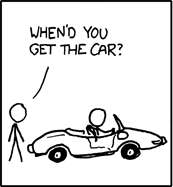
\includegraphics[width=3cm]{bilder/new_car_1.png}\\\vspace{20mm}
        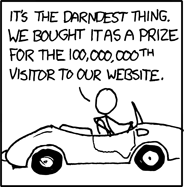
\includegraphics[width=3cm]{bilder/new_car_2.png}\\\vspace{20mm}
        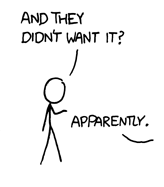
\includegraphics[width=3cm]{bilder/new_car_3.png}\\\vspace{20mm}
        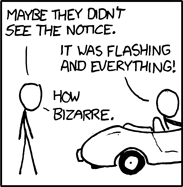
\includegraphics[width=3cm]{bilder/new_car_4.png}
    }
}

\subsection*{Drucken}

Zum Drucken kann man seine Dokumente auf einen speziellen Druck-Server\footnote{\url{http://drucker.uni-hd.de}} laden und dann an (fast) jedem der über den Campus verstreut aufgestellten Kopiergeräte ausdrucken.
Das zum Drucken benötigte Guthaben wird über die CampusCard abgerechnet, die man in den Mensen und in der \gls{UB} aufladen kann. Für größere Aufträge gibt es einen Druckerraum im Keller des \gls{URZ}, der von der Firma Ricoh betrieben wird.
Darüber hinaus bietet das URZ einen Poster-Druckservice\footnote{\url{http://www.urz.uni-heidelberg.de/service-katalog/druckservice/poster-service}} und einen 3D-Druckservice\footnote{\url{http://www.urz.uni-heidelberg.de/service-katalog/druckservice/3d-druckservice.html}} an.

\subsection*{CIP-Pools -- oder -- Internet ohne Notebook}
Rechnerräume stehen z.\,B.\ im \gls{KIP}, im \gls{PI}, im 1.~OG, im Keller der Institutsbibliothek der angewandten Mathe (\Gls{INF} 294), im \Gls{OMZ} und natürlich im \gls{URZ} bereit. In letzterem sogar mehrere -- wo noch Plätze frei sind erfahrt ihr am Infobildschirm (linker Eingang).

\subsection*{WLAN -- oder -- Internet mit Notebook}
\marginpar{
    \centering
    \vspace{1mm}
    \ifthenelse{\boolean{druckversion}}{
        
\includegraphics[width=3cm]{eduroam_sw.pdf}
    }{
        
\includegraphics[width=3cm]{eduroam.pdf}
    }
}
Am einfachsten und komfortabelsten ist der WLAN-Zugang über das eduroam-Netz.
Die Uni Heidelberg beteiligt sich an der eduroam-Initiative und bietet jedem Rechenzentrums-Nutzer einen entsprechenden Zugang. Damit könnt ihr nicht nur an vielen Stellen auf dem Campus kabellos ins Internet, sondern auch mehreren hundert Hochschulen und Forschungseinrichtungen in über 60 Ländern – einfach so.

Wie man sein Notebook konfigurieren muss, um eduroam zu nutzen ist auf den Webseiten des URZ\footnote{\url{http://www.urz.uni-heidelberg.de/zugang/eduroam/}} für die unterschiedlichsten Betriebssysteme sehr detailiert erklärt.

Neben eduroam bietet das URZ an einigen Stellen noch das Netwerk „UNI-HEIDELBERG“, das man mit einem VPN-Zugang nutzen kann, sowie das unverschlüsselte „UNI-WEBACCESS“, bei dem man sich in einem Captive Portal autentifiziert. Näheres hierzu bietet auch die URZ-Seite.%\footnote{\url{http://www.urz.uni-heidelberg.de/netz/laptop/wlan.html}}.

Sollte euch der ein WLAN-Zugang nicht mehr ausreichen, gibt es an einigen Orten auch kabelgebundene Zugänge mit mehr Bandbreite. Wo ihr Empfang haben solltet und wo sich LAN-Buchsen befinden, erfahrt ihr auf den Seiten des \gls{URZ}\footnote{\url{http://www.urz.uni-heidelberg.de/netz/laptop/verbreitung.html}}. Wer jetzt schon feuchte Hände bekommt und sich die niegelnagel neue externe Platte mit Inhalten aus zweifelhaften Quellen vollladen möchte, sei auf die Benutzerordnung\footnote{\url{http://urz-benutzerordnung.uni-hd.de}} verwiesen. Nach zu viel Traffic dreht euch das \gls{URZ} den Hahn ab und schaltet ihn erst wieder frei, wenn ihr bestätigt, dass ihr keine bösen Dinge damit anstellt.

\subsection*{VPN}
Um auf manche Dienste zugreifen zu können, müsst ihr euch im internen Uni-Netz befinden. Weil das von zu Hause irgendwie schwer ist, braucht ihr einen VPN-Tunnel. Damit stellt euer Rechner über einen Internetzugang eine Verbindung zur Uni her und es ist so, als würdet ihr mit einem LAN-Kabel in der Uni sitzen. Eine ausführliche Anleitung findet ihr online\footnote{\url{http://www.urz.uni-heidelberg.de/service-katalog/netzwerkdienste/vpn/}}, die neben allgemeinen Informationen auch Anleitungen zur Installation des \emph{Cisco Anyconnect VPN Client}, enthält. Hier aber dennoch die Kurzfassung:

Unter Linux könnt ihr einfach den \emph{openconnect} verwenden. Hier könnt ihr z.B. unter Ubuntu, Debian oder Mint das Paket \emph{network-manager-openconnect-gnome} nutzen und dort \emph{vpnsrv0.urz.uni-heidelberg.de} als Gateway und \emph{Deutsche\_Telekom\_Root\_CA\_2.pem} als CA Certificate einstellen.

Unter Windows\ldots Benutzt einfach kein Windows. Falls doch, nutzt den Cisco AnyConnect Client. Es gibt auch Alternativen, diese findet ihr auch auf den Seiten des Rechenzentrums.

Alternativ könnt ihr euch auch aus der Ferne direkt auf den Uni-Rechnern anmelden und so die dort installierte Software nutzen („Terminalserver“, „Remote Desktop“). Eine ausführliche Anleitung findet ihr online\footnote{\url{http://www.urz.uni-heidelberg.de/service-katalog/serverdienste/}}.

\subsection*{LSF}
Das LSF\footnote{\url{https://lsf.uni-heidelberg.de/}} ist das
Informationssystem der Uni. Hier findet ihr neben dem Vorlesungsverzeichnis und
Informationen zu Gebäuden und Personen auch eure Bescheinigungen,
beispielsweise für BAföG o.ä., euer Stammdatenblatt könnt ihr da auch
ausdrucken. Das braucht ihr, um später nachweisen zu können, das ihr auch
wirklich studiert habt.

Für einige Funktionen braucht ihr eine TAN. Diese müsst ihr euch einmal als
Liste ausdrucken. Das ist ein bisschen umständlich, sollte aber mit der
Anleitung, die ihr bei eurer Einschreibung bekommen habt, kein Problem sein.


%\section{Bibliotheken}
\mathphyssecnobar{Bibliotheken}%FIXME
Fachliteratur ist meistens unglaublich teuer. Um den totalen Ruin  der Studierenden zu vermeiden,
hat jede Universität Bibliotheken.  In Heidelberg ist die \gls{UB} dreigeteilt, und zwar
entsprechend  der Dreiteilung der Universität. Die für euch wahrscheinlich  interessanteste
Literatur über Mathe, Informatik und Physik befindet sich in  der Zweigstelle \gls{INF}~368, 3.~Stock.

Neben Physik-, Informatik-  und Mathebüchern können hier auch medizinische Literatur und Bücher zu allen anderen
Fakultäten, die im Neuenheimer Feld untergebracht sind, ausgeliehen werden. Im Hauptsitz der
\gls{UB} an der Peterskirche, Plöck~107-109, und der Campus-Bibliothek in Bergheim hingegen findet
sich die geisteswissenschaftliche Literatur sowie zahlreichen Jura- und VWL- Büchern. Bedingt durch
diese Dreiteilung wurde in Heidelberg sehr früh ein Computersystem („\gls{HEIDI}“
\footnote{\url{http://katalog.ub.uni-heidelberg.de}}) in der UB eingeführt. Mit Hilfe von Heidi und
eurer Uni-ID, die auf eurem Studiausweis steht, kann dort die gängige Fachliteratur ausgeliehen werden.
Übers Internet lässt sich auch direkt nach Büchern suchen, außerdem können ausgeliehene Bücher
online verlängert werden -- das kann einem durchaus den ein oder anderen Euro sparen, die
Mahngebühren bei überzogenen Fristen sind nämlich empfindlich teuer. Zu Semesterbeginn finden in der
UB Einführungskurse in Heidi statt, die jedoch nur bedingt sinnvoll sind, weil das System sehr
übersichtlich und intuitiv aufgebaut ist und sich größtenteils selbsterklärend bedienen lässt.

Wer weiterführende spezielle Fachliteratur sucht, muss sich an die Seminarbibliotheken der
einzelnen Fakultäten halten. Für Mathe- und Informatik-Literatur befindet sich die Seminarbibliothek
im Gebäude \gls{INF}~294 (rechter Eingang und dann geradeaus durch). Spezielle Physikbücher stehen
in der Physik-Seminarbibliothek im Philosophenweg~16. Einziger Nachteil: Die zahlreichen Bücher und
Spezialzeitschriften können hier nur zum Kopieren ausgeliehen werden. Wenn ein Buch in der UB
ausgeliehen ist, dann lohnt es sich manchmal auch, zur Stadtbücherei in der Poststraße zu gehen. Sie
wurde 1993 aufwendig umgebaut und besitzt seitdem ebenfalls ein „neues“ Computersystem. Zum Anmelden
braucht man nur einen Personalausweis. Die Ausleihe ist seit dem Umbau allerdings nicht mehr
kostenlos (\EUR{10}/Jahr).\\ Weitere Information kannst du auch direkt bei der Stadtbücherei
einholen\footnote{\url{http://www.stadtbuecherei-heidelberg.de}}.

In der Schulgasse~6 (3. Stock) gibt es zusätzlich noch die Studierendenbibliothek. Über zwei
Etagen sind hier vorwiegend geisteswissenschaftliche Bücher aufgereiht. Ein sehr fähiger und netter
Bibliothekar hilft beim Suchen. Die beiden letzten Bibliotheken eignen sich natürlich insbesondere
auch dazu, einfach mal nur zu schmökern.

\begin{table*}[htb]
\centering

% Diese Tabelle wurde mühsam angeordnet. Bitte nicht umbrechen, sondern scrollen!
%~ \newcommand{\bibKIP}{}
\begin{tabular}{lll@{ -- }l@{\quad}r@{ -- }l@{ Uhr}}
\toprule
Name                                    & Adresse                                                                                                                       & \multicolumn{4}{l}{"Offnungszeiten}    \\
\midrule
\multirow{3}{*}{\gls{UB} (Ausleihe)}    & \multirow{1}{*}{\href{http://www.openstreetmap.org/?mlat=49.40966&mlon=8.70594&zoom=17&layers=M}{Plöck 107-109 (Altstadt)}}   & Mo & Fr                    & 9    & 19 \\[-0.7\defaultaddspace]
                                        & \multicolumn{1}{c}{und}                                                                                                                                                \\[-0.7\defaultaddspace]
                                        & \multirow{1}{*}{\href{http://www.openstreetmap.org/?mlat=49.41767&mlon=8.66836&zoom=17&layers=M}{INF 368, 3. Stock (Feld)}}   & \multicolumn{2}{l}{Sa}     & 9    & 13 \\
\cmidrule{1-6}
\multirow{5}{*}{\gls{UB} (Lesesaal)}    & \multirow{2}{*}{\href{http://www.openstreetmap.org/?mlat=49.40966&mlon=8.70594&zoom=17&layers=M}{Plöck 107-109 (Altstadt)}}   & Mo & Fr                    & 8:30 & 1 \\
                                        &                                                                                                                               & \multicolumn{2}{l}{Sa}     & 9    & 1 \\[-0.7\defaultaddspace]
                                        & \multicolumn{1}{c}{}                                                                                                                                                \\[-0.7\defaultaddspace]
                                        & \multirow{2}{*}{\href{http://www.openstreetmap.org/?mlat=49.41767&mlon=8.66836&zoom=17&layers=M}{INF 368 (Feld)}}             & Mo & Fr                    & 8:30 & 22 \\
                                        &                                                                                                                               & Sa & So                    & 9    & 22 \\
\cmidrule{1-6}

\multirow{2}{*}{Angewandte Mathe}       & \multirow{2}{*}{\href{http://www.openstreetmap.org/?mlat=49.41905&mlon=8.67117&zoom=17&layers=M}{INF 294}}                    & Mo & Fr                    & 8    & 22 \\
                                        &                                                                                                                               & \multicolumn{2}{l}{Sa}     & 9    & 19 \\
\cmidrule{1-6}
\multirow{2}{*}{Physik}                 & \multirow{2}{*}{\href{http://www.openstreetmap.org/?mlat=49.41479&mlon=8.69686&zoom=17&layers=M}{Philosophenweg 16}}          & Mo & Do                    & 9    & 19 \\
                                        &                                                                                                                               & \multicolumn{2}{l}{Fr}     & 9    & 17 \\
\cmidrule{1-6}
\gls{KIP}                               & \href{http://www.openstreetmap.org/?mlat=49.41644&mlon=8.67168&zoom=17&layers=M}{INF 227 (3. Stock)}                          & Di & Do                    & 14    & 17 \\
\cmidrule{1-6}
\multirow{3}{*}{Stadtbücherei}          & \multirow{3}{*}{\href{http://www.openstreetmap.org/?mlat=49.40638&mlon=8.6866&zoom=17&layers=M}{Poststraße 15}}               & Di & Fr                    & 10   & 20 \\
                                        &                                                                                                                               & \multicolumn{2}{l}{Sa}     & 10   & 16 \\
                                        &                                                                                                                               & \multicolumn{4}{l}{Montags geschlossen!}\\
\cmidrule{1-6}
\multirow{2}{*}{Studibücherei}          & \multirow{2}{*}{\href{http://www.openstreetmap.org/?mlat=49.41082&mlon=8.70733&zoom=17&layers=M}{Schulgasse 6}}               & Mo & Do                    & 11   & 17 \\
                                        &                                                                                                                            & \multicolumn{2}{l}{Fr}     & 11   & 14 \\
\bottomrule
\end{tabular}

\end{table*}


\section{Arbeitsraum}
Seit dem letzten Semester gibt es am Philosophenweg 12 in den Räumen 60/61
einen studentischen Arbeitsraum, den wir vor allem für euch eingerichtet haben.
Das Tolle daran ist, dass drei TutorInnen eingestellt wurden, um Euch bei
Fragen und Problemen zur Verfügung zu stehen. Das läuft sehr gut und wir haben
viel positive Resonanz bekommen, besonders für die TutorInnen. Das Konzept
sieht vor, dass wir sowohl einen kleinen Stillarbeitsbereich, aber auch einen
Gruppenarbeitsraum für Diskussionen haben. Neben ein paar Standardbüchern gibt
es dort auch eine Kaffeemaschine und einen Wasserkocher. In der Zukunft soll
der Raum auch noch ausgebaut werden, allerdings muss er nun erst einmal über
einen längeren Zeitraum angenommen werden, bevor noch mehr Geld dort
hineingesteckt wird. Besonders oft verliert man nämlich im
Übungszetteldschungel den Überblick, was wirklich wichtig ist. Genau dabei
können einem aber oft ältere Studis helfen. Auch sollen sie dir helfen deine
Übungszettel besser zu lösen, indem sie hilfreiche Tipps geben.

Um Rückmeldung dazu zu geben, könnt ihr einfach kurz die Umfrage
\footnote{\url{http://goo.gl/forms/iDhmpx8kHx}} ausfüllen. Das hilft uns bei
den Verhandlungen mit der Fakultät enorm und außerdem können wir so abschätzen,
was die größten Probleme sind.

Der Raum ist während der Vorlesungszeit immer Montags bis Donnerstags von 14
bis 19 Uhr und Freitags bis 17 Uhr geöffnet. Falls dir also das KIP zu voll
ist, du eh eine Übungsgruppe am Philosophenweg hast oder einfach am
Philosophenweg Lust auf Kaffee hast, komm doch einfach mal vorbei.

\newpage
%\section{Was tun bei Problemen}
\mathphyssecnobar{Was tun bei Problemen}%FIXME
\label{dschungel}
Da seid ihr also: ordentlich immatrikuliert, auch schon eine Bleibe gefunden (zumindest vorläufig), möglicherweise bereits Bekanntschaft mit diversen Ämtern und Behörden geschlossen. Und nun kann es eigentlich losgehen mit dem „lustigen Studentenleben“. Oder?

Aber was ist das eigentlich, studieren? Wie wird das Studium im ersten Semester aussehen? Wie lernt man denn an der Uni, wenn einem niemand so richtig vorschreibt, was wann wie zu machen ist? Überall hört man von Studiengebühren -- betrifft mich das eigentlich? Und wie ist das mit dem BAfÖG? Wann muss ich meine ersten Prüfungen ablegen? Wie kann ich Studium und Job unter einen Hut bringen? Bleibt neben dem Studium überhaupt noch Zeit, etwas anderes zu machen?

Was im Weltall gilt, gilt auch in der geistigen Galaxie: Don't panic! Der Überblick, den ihr jetzt noch nicht habt, stellt sich noch ein. Vor allem seid ihr nicht allein. Ein Anliegen dieses Heftes ist es, euch die Anlaufstellen aufzuzeigen, wie z.\,B.\ die Zentrale Studienberatung, Sozial- und Rechtsberatung, oder die Psychosoziale Beratungsstelle des Studentenwerks\footnote{Überblick über die einzelnen Beratungsangebote:\\\url{http://www.uni-heidelberg.de/studium/imstudium/beratung.html}}.

Worüber ihr euch klar werden solltet, ist, was ihr euch vom Studium erwartet. Fragt euch also: Warum studiere ich? Welches Berufsziel schwebt mir vor? Warum gerade dieses Fach? Ihr müsst diese Entscheidungen für euch selbst treffen und Prioritäten setzen -- der Stundenplan bietet keine Anleitung dazu, die eigenen Fähigkeiten und Erwartungen im Studium umzusetzen.\enlargethispage{\baselineskip}%FIXME
%\begin{minipage}{1.5\textwidth}
%\hspace{-5mm}
%        \includegraphics[width=6cm]{bilder/dschungelbuch_1.png}
%        \hspace{10mm}
%        \includegraphics[width=6cm]{bilder/dschungelbuch_2.png}\\\vspace{5mm}
%\end{minipage}

%\section{Die kleine BAföG-Liste}
\mathphyssecnobar{Die kleine BAföG-Liste}%FIXME

\paragraph{Soll ich BAföG beantragen?}
JA! Ob du anspruchsberechtigt bist, lässt sich nur schätzen. Vom BAföG sind 50\% Zuschuss, die andere Hälfte zinsloses Darlehen. Zurückzuzahlen muss man es  frühestens drei Jahre nach Studienabschluss, aber nur ab einer bestimmten Einkommenshöhe. Rückzahlungsaufschub ist jederzeit ohne Nachteile möglich!

\paragraph{Wie viel gibt es und wie lange und ab wann?}
Maximal \EUR{648} (ohne Kind, abhängig von Miet(e)verhältnis, Einkommen der Eltern, eigenem Vermögen, Krankenversicherung, Geschwistern, etc.)
Die Förderungsdauer richtet sich nach der Regelstudienzeit (Bachelor und konsekutiver Master = 6 + 4, aber es gibt fachspezifische Ausnahmen), Anspruchszeit zählt ab Immatrikulation und ist nicht aufsparbar! Die Auszahlung geschieht in der Regel erst, wenn Bescheid eingegangen ist, bei dringender Bedürftigkeit ist  ggf. Vorschuss (in voller BAföG-Höhe, der hinterher verrechnet wird) möglich.

\paragraph{Wo und bis wann muss ich den Antrag stellen?}
Das geht beim BAföG-Amt des Studentenwerks im Marstallhof 3 je Mo.\ -- Fr.\ 8 – 18 Uhr. Kurzberatung im Neuenheimer Feld gibt es Mo.\ – Do.\ 10.00 -- 17.00 Uhr und Fr.\ 10.00 -- 15.00 Uhr. Das macht man am besten sobald man die Immatrikulationsbescheinigung hat, denn BAföG gibt es erst vom Antragsmonat an, wobei der frühestmöglichste Termin der Semesteranfang ist.

\paragraph{Was muss ich beim Antrag beachten?}
Antrag so früh wie möglich stellen, weil es teilweise zu langen Bearbeitungszeiten kommen kann. Der Antrag sollte idealerweise vollständig sein, da so Rückfragen entfallen und der Antrag schneller bearbeitet werden kann. Ansonsten gilt: lieber schnell beantragen und Papiere nachreichen. Die Angaben sollten wahrheitsgemäß sein, denn das Amt kann die Finanzdaten prüfen.

\paragraph{BAföG und nun? Was sonst noch zu beachten wäre.}
Man muss nach dem vierten Fachsemester seine Studienleistungen bescheinigen lassen!
Familiäre und persönliche wirtschaftliche Veränderungen immer sofort melden (Schwester/Bruder in Ausbildung/Arbeit, Arbeitslosigkeit, etc.)
Es gibt auch Auslands-BAföG und viele sonstige Ausnahmen, zu denen man sich am besten beraten lässt! Es kann sich lohnen!
Zuverdienst bis maximal \EUR{4\,880} Brutto im Jahr oder \EUR{450} im Monat (mit vielen Ausnahmen).\\[5mm]

\noindent Abschließend: Nutzt die Sprechstunde vom Sozialreferat des \gls{StuRa} (Mi.\ und Fr.\ 11 -- 13 Uhr). Die helfen Euch beim Antrag, erklären Ausnahmen, geben Tipps (um spätere Probleme zu vermeiden, bei denen sie natürlich auch helfen).

% !TEX ROOT = ../ersti.tex
%\section{Studium im Ausland}
\newpage\mathphyssecnobar{Studium im Ausland}%FIXME
Man hört immer wieder von den tollen Erfahrungen und Möglichkeiten, die ein
Studium im Ausland bietet. Die Leute schwärmen davon, wie schön es an der Uni
so-und-so war. Aber wie kommt man überhaupt dahin?

In den Bachelor-Studienordnungen der Physik und der Mathe heißt es, „Bei der
Anerkennung von Studienzeiten, Studien- und Prüfungsleistungen, die außerhalb
Deutschlands erbracht wurden, sind die von Kultusministerkonferenz und
Hochschulrektorenkonferenz gebilligten Äquivalenzvereinbarungen sowie
Absprachen im Rahmen von Hochschulpartnerschaften zu beachten. Bei Zweifeln an
der Gleichwertigkeit kann die Zentralstelle für ausländisches Bildungswesen
gehört werden.“ Das ist nicht sonderlich hilfreich, wenn man sich nicht
unbedingt durch Tonnen von Gesetzestext quälen will. Auf der Homepage der
jeweiligen Fakultät findet ihr eine Liste von Unis, mit denen
Austauschprogramme laufen (die also anerkannt werden), einige generelle Infos
und ein paar Erfahrungsberichte, die ihr bei Interesse anschauen solltet.
Die Gleichwertigkeit von Studienleistungen muss allerdings nicht von euch 
überprüft werden, die Beweispflicht liegt bei der Fakultät. Lasst euch also 
nicht beirren und hört im Zweifel die Veranstaltung im Ausland einfach, die
sollen erst mal zeigen, dass das nicht das gleiche war.

Allerdings sollte ein Auslandssemester im Moment nicht euer erstes Problem
sein -- während der ersten beiden Semester ist es ganz einfach fachlich nicht
möglich. Bis zur Einführung der Bachelor- und Masterstudiengänge konnte man
(wenigstens in der Mathe) an diesen Programmen nur nach abgeschlossenem
Grundstudium teilnehmen, inzwischen wird der Zeitraum letztes Jahr
Bachelor/erstes Jahr Master empfohlen. Das bedeutet, dass ihr nach dem zweiten
Semester damit beginnen solltet, euch umzuschauen, insbesondere in Bezug auf
Bewerbungsvoraussetzungen und -fristen.

Auslandsbafög müsst ihr übrigens separat beantragen, die Zuständigkeit dafür

hängt vom jeweiligen Ausland ab, eine Liste der zuständigen Ämter findet man
z.B. unter \url{Auslandsbafög.de}. In Heidelberg kann man sich auch direkt
an das Dezernat Internationale Beziehungen (früher Akademisches Auslandsamt, AAA)\footnote{\url{http://www.uni-heidelberg.de/studium/kontakt/auslandsamt/}} wenden, das ihr in der Seminarstraße 2 findet. Ihr müsst dann ins Zimmer 139.

\paragraph{Öffnungszeiten} Mo. -- Do. 10 -- 15 \qquad Fr. 10 -- 13



%%%%%%%%%%%%%%%%%%%%%%%%%%%%%%%%%%%%%%%%%%%%%%%%%%%%%%%%%%%%%%%%%%%%%%%%%%%%%
\chapter{\dots und in der Stadt}
\section{Wohnen in Heidelberg}

\sidebar{
    \chaptersidebarpushdown
    \centering
    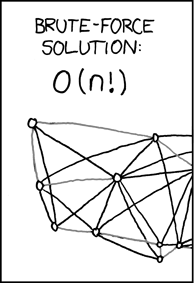
\includegraphics[width=3cm]{bilder/travelling_salesman_problem_1.png}\\\vspace{10mm}
    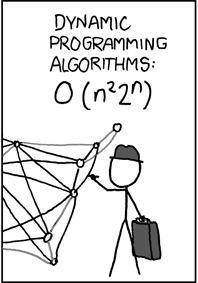
\includegraphics[width=3cm]{bilder/travelling_salesman_problem_2.png}\\\vspace{10mm}
    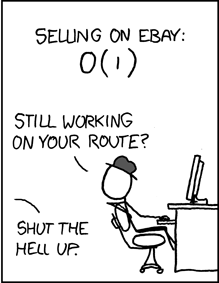
\includegraphics[width=3cm]{bilder/travelling_salesman_problem_3.png}
}


Wie in jeder Unistadt, so ist es auch in Heidelberg schwer, zu Anfang des Semesters
ein Zimmer zu finden, das bezahlbar ist und möglichst zentral liegt. Im Durchschnitt
muss man in Heidelberg mit Lebenshaltungskosten von ca. \EUR{650} (inklusive Miete)
pro Monat rechnen.

Am günstigsten wohnt man immer noch im Studentenwohnheim, dort muss man mit Mieten
von ca. \EUR{168 -- 300} pro Monat rechnen. Auch WG-Zimmer sind teilweise recht
günstig zu bekommen, in der Regel jedoch teurer als ein Zimmer im Wohnheim.

Die Idee, eine eigene WG zu gründen, liegt meist sehr nahe, jedoch wird man schnell
merken, dass das gar nicht so einfach ist. Oft werden Ehepaare ohne Kinder bevorzugt
oder ein Zimmer entpuppt sich als Durchgangszimmer. Egal, für was ihr euch
entscheidet: plant viel Zeit ein und lasst nicht locker!

Nun aber zur konkreten Zimmersuche: es gibt mehrere Möglichkeiten, ein Zimmer in
Heidelberg zu finden. Das Studentenwerk bietet mehrere Anlaufstellen: In der
Altstadt das Info-Café International in der Triplex-Mensa direkt am Uniplatz, im
Neuenheimer Feld im Infocenter der Zentralmensa. In den Mensen, aber auch in den
einzelnen Instituten empfiehlt es sich, die schwarzen Bretter abzuklappern und nach
privaten Aushängen Ausschau zu halten oder selbst Anfragen anzuhängen. Weitere gute
Quellen für Zimmerangebote sind natürlich die regionalen Zeitungen. Das wären u.a.
„Sperrmüll“, erscheint immer dienstags und freitags und die Rhein-Neckar-Zeitung,
mittwochs und samstags mit großem Immobilienteil.
%Aufpassen müsst ihr bei Makler-Vermittlungen, hier müsst ihr zusätzlich zwischen
%ein und zwei Monatsmieten Provision zahlen.
Eine eigene Anzeige kann natürlich nie schaden. Zu guter Letzt gibt es noch das
Internet, das eine Fülle an Portalen\footnote{z.B. \url{wg-gesucht.de}} zur
Wohnungssuche bietet.

\clearpage

\subsubsection{Wohnheime}
In und um Heidelberg gibt es ca. 50 Wohnheime des Studentenwerks, im Wintersemester
werden ca. ein Fünftel aller dieser Zimmer neu vermietet. Die Auswahl erfolgt nach
sozialen Kriterien wie zum Beispiel Heimatferne, Verdienst der Eltern,
Wohnverhältnisse usw. Die Wohnzeit ist auf sechs Semester begrenzt, aber es gibt
viele Möglichkeiten, diese zu verlängern, zum Beispiel durch Sonderaufgaben im
Wohnheim, Härtefälle etc. Die maximale Wohnzeit kann auf insgesamt zehn Semester ansteigen, was
durchaus vorkommt. Je nach Wohnheim gibt es Einzelzimmer mit Stockwerksküche und
-Bad, die ihr dann mit jeweils 15-20 Leuten teilt (was mittlerweile aber eher selten
ist), Einzelzimmer in 2er, 3er oder 4er WGs oder sogar Einzelappartments. Die Zimmer
sind in der Regel nicht sehr groß (11--16 \squaren\metre), aber ausreichend. Nachteile von
Wohnheimen können die teilweise sehr unterschiedlichen Vorstellungen von Hygiene
sein, ein hoher Lärmpegel und immer wieder neue Überraschungen. Allerdings bietet
ein Wohnheim vor allem für Leute, die neu in der Stadt sind den großen Vorteil sehr
schnell viele Leute kennen zu lernen, außerdem muss man sich um Reparaturen nicht
selbst kümmern. Es gibt keine konkreten Bewerbungsfristen. Die Bewerbung sollte
allerdings bis 1. Juli für das Wintersemester und bis 1. Januar für das
Sommersemester eingegangen sein, weil dann mit der Zimmereinteilung und dem Versand
der Mietverträge begonnen wird. Später eingehende Bewerbungen haben weitaus
geringere Chancen und Auswahlmöglichkeiten. Antragsformulare gibt es in den
Infocentern des Studentenwerks oder im Internet\footnote{\url{http://www.studentenwerk.uni-heidelberg.de}}.
Dort gibt es auch eine vollständige Liste aller Wohnheime des Studentenwerks.

Auch private, kirchliche oder sonstige Träger bieten Zimmer in Wohnheimen an, für
diese müsst ihr euch direkt beim Wohnheim bewerben, nicht beim Studentenwerk. Eine
Liste findet ihr aber beim Studentenwerk\footnote{\url{http://studentenwerk.uni-heidelberg.de/download/pdf/wo-in-hd-andere-traeger-de.pdf}}.


% !TEX ROOT = ../ersti.tex
\newcounter{zahl}
\newcommand{\place}[4]{\item[(\stepcounter{zahl}\thezahl) #1](#2)\\ #3\\\emph{Preis:} #4}

% Indikator für Frauenanteil? Nein!

\section{Bars, Kneipen \& Diskotheken}
\subsection*{In der Altstadt:}
Preis: $\star$ teuer, $\star\ \star$ noch teurer, $\star\ \star\ \star$ extrem teuer


\begin{description}

%    \place{Alfredo}{Untere Straße}{Wirklich sehr leckere Pizza, der Chef sorgt für den echt italienischen Flair.}{$\star$}

    \place{Cave 54}{Krämergasse 1}{(Deutschlands ältester) Jazzkeller. Kostet am Wochen\-ende Eintritt, hat dafür allerdings noch nach 3 Uhr geöffnet.}{$\star\ \star$}

%    \place{Coyote}{Hauptstraße}{Einer der Orte, um eine Kneipentour durch die Altstadt starten zu lassen. Weizenbier, Cocktails und Shots sind brauchbar und brauchen nicht ewig.}{$\star\ \star$}

    \place{Destille}{Untere Straße}{Große Auswahl an Shots. Kultiger Laden mit ständig wechselnder Dekoration.}{$\star\ \star$}

    \place{Eckstein}{am Fischmarkt 3}{Abgefahrene Kneipe. Je nach Wochentag ändert sich das Programm. Es gibt jedoch immer einen Kicker und reichlich Platz. Drei Mal wöchentlich Zaubershows.}{$\star\ \star$}

    \place{Hard Rock Cafe}{Hauptstraße 142}{Montags Bier für \EUR{1}, ab 18 Uhr Cocktails für \EUR{4}. Musik wie man es erwartet, durchgehend Rock.}{$\star$}

%    \place{Havanna}{Neckarstaden 24}{Cocktailbar mit Möglichkeit zum Salsa tanzen.}{$\star\ \star\ \star$}

    \place{Hemmingways}{Fahrtgasse 1}{Hier lässt es sich das gesamte Jahr draußen sitzen, dank warmen Decken und Heizstrahlern. Außerdem kann man wunderbar den Neckar beobachten.}{$\star\ \star$}

    \place{Karls}{Lauerstraße 7-9}{Kneipe mit Billardtisch und Dartscheibe. Gut um sich voll\/laufen zu lassen oder einfach nur zu versacken.}{$\star\ \star$}

    \place{Karlstorbahnhof}{Am Karlstor\,/\,S-Bahnhof Altstadt}{Richtig gute Diskothek (Nicht nur; im Gebäude gibts auch Theater, Lesungen ect. - viel Kultur) mit sehr variabler Musik. Was zum tanzen und weniger zum trinken, denn die Preise können sich meistens sehen lassen, genauso der Eintritt}{$\star\ \star\ \star$}

    \place{Marstall}{Marstallhof}{Keine typische Kneipe, vielmehr Mensa mit Bier. Trotzdem gut geeignet sich zu treffen, zum Vorglühen und entscheiden, wo die weitere Party ihren Anfang nehmen soll.}{$\star$}

%    \place{Maxbar}{Marktplatz 5}{Hier gibt es des öfteren Live-Musik}{$\star\ \star$}

    \place{Medoc}{Bismarckplatz}{Cafe Restaurant das für ca. \EUR{5} wechselnde Mittagsgerichte anbietet. Man kann draußen sitzen und den Betrieb auf dem Bismarckplatz beobachten.}{$\star\ \star$}

    \place{Mels}{Heiliggeiststr. 1}{Gewölbekeller in dem seit Jahren die selbe Musik läuft, aber zumindest weiß man dann, was einen erwartet. Haben unter der Woche immer sehr gute Spezialangebote z.B. Dienstags 123-Party (Bier \EUR{1}, Weizen 2, Cocktails 3).}{$\star\ \star$}

    \place{Mohr}{Untere Straße}{Hoher Mediziner*innen Anteil, Einlass erst ab 20 Jahren und spät abends meist so voll, dass man gar nicht mehr rein kommt. Drinnen wird dafür allerdings auf den Tischen getanzt.}{$\star\ \star$}

    \place{Orange}{Ingrimmstraße 26a}{Eine Kneipe wie ein Wohnzimmer. Eng aber gemütlich. Es gibt sogar Brettspiele.}{$\star\ \star$}

%    \place{Palmbräugasse}{Untere Straße}{Hier gibts das selbstgebraute Palmbräu. Palmen gehören zwar nicht typisch zu Heidelberg, aber die Schnitzel in der Palmbräugasse.}{$\star\ \star$}

    \place{Regie}{Theaterplatz}{Riesenauswahl an Cocktails, die nach Filmen benannt sind.}{$\star\ \star\ \star$}

    \place{Reichsapfel}{Untere Straße}{Sehr geräumig. Moderner Vorderbereich und urigere Atmosphäre im hinteren Teil, welcher über den Innenhof zugänglich ist. Dort findet man oft Platz wenn sonst alles voll ist.}{$\star\ \star$}

    \place{Sonderbar}{Untere Straße}{Jede nur erdenkliche Form von Absinth, auch viel guten Rum und Whisky. Immer ordentlich was auf die Ohren (Hard \& Heavy). Keine Angst vor dem Wirt, einfach nicht auf den Mund gefallen sein. Oft sehr voll und vollgeräuchert.}{$\star\ \star$}

    \place{Tangente}{Kettengasse 23}{Hoher Jurist*innenanteil und teils ältere Menschen. Türsteher und Gesichtskontrolle, dafür aber kein Eintritt. Hier kann man bis in die frühen Morgenstunden tanzen, mann sollte allerdings keine Platzangst haben.}{$\star\ \star$}

    \place{Vater Rhein}{Untere Neckarstraße 20}{Legendär für seine \EUR{1,90}-Spaghetti bis halb drei. Hier lässt sich der Abend gemütlich ausklingen.}{$\star$}

\end{description}

% trim=l b r t
\hspace*{-6mm}
\altstadtkarte

%%%%%%%%%
\subsection{In den Stadtteilen:}
\begin{description}

    \place{Alt Hendesse}{Muhltalstraße 4}{Ist eigentlich ein Restaurant, hat im Sommer aber auch einen netten Biergarten. Die Portionen sind groß und lecker. Stammlokal einiger Matheprofs.}{$\star\ \star$}

    \place{Bar 133}{Wohnheim \gls{INF} 133}{Wohnheimsbar, eigentlich nur für Bewohner der 1xx Wohnheime. Mittwochs und sonntags geöffnet mit gutem Angebot, günstigen Cocktails und Tischkicker. Immer wieder für einen Absturz gut.}{$\star$}

%    \place{Breidenbach Studios}{Hebelstraße 18}{Absoluter Hipster-Laden: Ehemalige Gasflaschenhandlung, die zu einem Künstlerhaus und Coworking-Space umgebaut wurde. Hier finden immer wieder großartige Partys statt.}{$\star\ \star\ \star$}

    \place{Cappuchino}{Bergheimer Straße 8}{Hippe Mischung von Kaffeehaus mit lautem Elektro.}{$\star\ \star$}

    \place{Halle 02}{Bahnstadt}{Electrofreunde werden hier ihren Spaß haben, es gibt aber auch viele Mainstream Partys. Meistens sind diese auch recht voll und es herrscht gute Stimmung. Ab und zu spielen auch bekanntere Bands.}{$\star\ \star$}

    \place{O'Reilly's}{Brückenkopfstraße 1}{Irish Pub mit Karaokee.}{$\star\ \star\ \star$}

    \place{schwimmbad club}{INF, am Tiergartenschwimmbad}{Hier läuft echt alles. Ob House, Latin, 80s oder Rock, es findet sich immer das passende Event, das mit \EUR{4}\,–\,\EUR{8} Eintritt auch halbwegs bezahlbar ist. Besonderes Sternchen ist das Schwarze Schwimmbad jeden 4. Samstag im Monat.}{$\star\ \star$}

    \place{P11}{am Römerkreis}{Nettes Café, dass Abends bis etwa 1 Barbetrieb hat. Geile Tapete!}{$\star\ \star$}

    \place{Villa Nachttanz}{Im Klingenbühl 6}{Alternativer Kulturverein -- rechnet mit allem außer Mainstream. Sehr günstig, mit Lagerfeuer im Garten. Lohnt sich jedes mal.}{$\star$}

    \place{Ziegler}{Bergheimer Straße 1}{Kneipe mit Disco, welche allerdings Eintritt kostet und auch sonst recht hohe Preise hat. Oft auch Live Musik}{$\star\ \star\ \star$}

    \place{Zwitscherstube}{Blumenstraße 25}{Urige Kneipe mit Alt, Kölsch und original Underberggürtel. Hier kommen vor allem Fußballfans auf ihre Kosten. Wenn kein Fußball läuft kann man super Skat spielen.}{$\star$}


\end{description}


%\section{Geschichte der Ruprecht-Karls-Universität Heidelberg}
\label{geschichte}
Die Ruperto Carola wurde im Jahre 1386 mit päpstlicher Genehmigung von Kurfürst 
Ruprecht I. als Ruprechts-Universität Heidelberg gegründet. Sie ist die Dritte im 
Heiligen römischen Reich deutscher Nation nach Prag und Wien, also die älteste in 
den Grenzen des heutigen Deutschlands. Aufgrund der Spaltung der Kirche war es 
nötig geworden, eine Ausbildung eigener Theologen zu ermöglichen, da 
Sorbonne-Absolventen nicht mehr im römischen Reich in kirchliche Dienste treten durften.
Marsilius von Inghen, der Gründungsrektor, wegen der Kirchenspaltung aus Paris geflohen, eröffnet die Universität im Oktober 1386 mit einer feierlichen Messe. Die Anfänge 
der Universität sind durch erhebliche Raumprobleme gekennzeichnet: Kirchen und 
Klostersäle werden für Vorlesungen genutzt. Erst später können eigene Gebäude für 
die Lehre errichtet werden. Im Zuge der Universitätsgründung werden die 
Stiftsbibliotheken der umliegenden Klöster vereinigt, um eine einigermaßen solide 
Ausbildung zu gewährleisten; die Büchersammlung wird dabei kontinuierlich erweitert 
(zum Beispiel durch vererbte Bestände der Augsburger Handelsfamilie Fugger) und im 
16. Jahrhundert zur Bibliotheca Palatina vereinigt.

1556 wird die Universität im Zuge der Reformation in eine evangelische 
Landeshochschule umgewandelt. Kurfürst Ottheinrich führt normale bürgerliche 
Kleidung statt der sonst üblichen geistlichen Tracht für Studierende ein. Auch die 
finanzielle Situation verbessert sich stark durch die Übertragung von Kirchengut an 
die Universität. Später wird die Universität sogar als calvinistische Hochschule im 
„deutschen Genf“ bezeichnet. So blüht sie bis 1618 auf, die Studierendenzahlen wachsen, 
auch wenn die Universität im Vergleich zu anderen deutschen Universitäten immer noch 
zu den kleinen zählt.
\marginpar{
    \centering{
        \vspace{-50mm}
        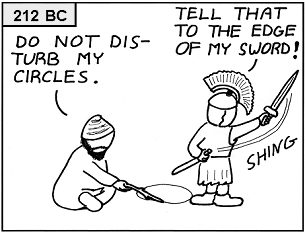
\includegraphics[width=3cm]{bilder/a_wise_man_once_said_1.PNG}\\\vspace{13mm}
        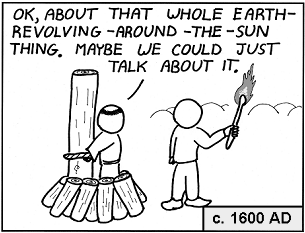
\includegraphics[width=3cm]{bilder/a_wise_man_once_said_2.PNG}\\\vspace{13mm}
        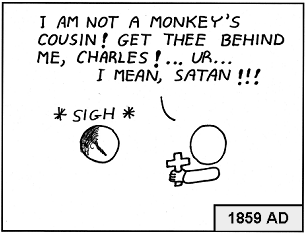
\includegraphics[width=3cm]{bilder/a_wise_man_once_said_3.PNG}\\\vspace{13mm}
        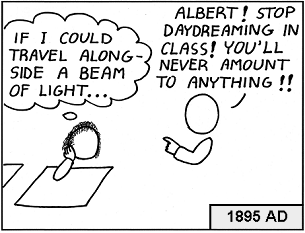
\includegraphics[width=3cm]{bilder/a_wise_man_once_said_4.PNG}\\\vspace{13mm}
        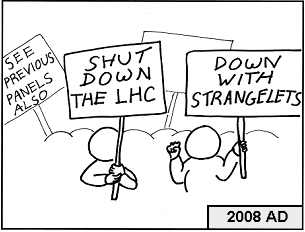
\includegraphics[width=3cm]{bilder/a_wise_man_once_said_5.PNG}\\\vspace{13mm}
        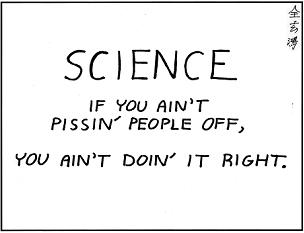
\includegraphics[width=3cm]{bilder/a_wise_man_once_said_6.PNG}\\\vspace{13mm}
    }
}



Während des 30-jährigen Kriegs wird die Universität ziemlich stark beschädigt und 
der Lehrbetrieb muss immer wieder unterbrochen werden bis sie schließlich 1652 
wiedereröffnet wird. Doch der Frieden hält nicht lange an. Im Zuge des Pfälzer 
Erbfolgekrieges wird die ganze Stadt Heidelberg verwüstet. Die Bibliotheca Palatina 
wird als Kriegskostenersatz an den Papst verschenkt. 

%% der lehrbetrieb wurde eingestellt und eigentlich gabs die Uni nicht Davon erholt sich die 
%Universität nur sehr langsam.

Mitte des 18. Jahrhunderts beginnen sich die Naturwissenschaften zu etablieren. 
Zuerst als Teil der philosophischen Fakultät entsteht 1752 der Lehrstuhl für 
Mathematik und Experimentalphysik. Diese Entwicklung setzt sich 1802 mit dem 
Übergang Heidelbergs an Baden fort. Die Universität erweitert nach dem ersten 
Großherzog von Baden ihren Namen zu „Ruprecht-Karls-Universität Heidelberg“. Sie ist 
von jetzt an staatlich finanziert und wird komplett reorganisiert. Die 
Naturwissenschaftlich-Mathematische Fakultät trennt sich von der Philosophischen und 
entwickelt sich vor allem unter dem Einfluss von Robert Bunsen, Gustav Kirchhoff und 
Hermann von Helmholtz. Georg Wilhelm Friedrich Hegel lehrt zwei Jahre an der 
philosophischen Fakultät, die medizinische Fakultät zieht Patienten aus aller Welt an. 
Trotzdem wird Heidelberg vor allem als juristische Universität gesehen. Auch kommt 
es in dieser Zeit zu Entwicklungen in der Frauengleichstellung. Im Jahr 1895 
promoviert Katharina Windscheid als erste Doktorandin in Heidelberg. 1900 wird 
Georgine Sexauer als erste Studentin immatrikuliert und 1923 wird Gerta von Ubisch 
als Professorin für Botanik habilitiert.

Im 20. Jahrhundert setzt sich dieser Trend fort. Heidelberg ist eine weltoffene und 
liberale Universität, an der man auch eine große Zahl von ausländischen Studierenden 
findet. Das interdisziplinäre Gespräch wird gesucht, was der Uni ihren typischen 
„Heidelberger Geist“ verleiht, der in der Weimarer Republik auch häufig als 
demokratischer Geist bezeichnet wird.

Trotzdem wird die Studierendenschaft im Verlauf des 20. Jahrhunderts immer radikaler 
und mit dem Erstarken des Nationalsozialismus werden viele ProfessorenInnen entlassen und 
Studierende aus politischen und rassistischen Gründen ausgeschlossen. Bei der 
Bücherverbrennung auf dem Universitätsplatz 1933 nehmen viele Mitglieder der 
Universität aktiv teil; die Ruperto Carola ist als braune Universität verrufen.
Die Athene wich dem Hakenkreuz, der lebendige Geist dem deutschen. 

Nach dem zweiten Weltkrieg ist die Universität äußerlich zerstört, gravierender sind jedoch die Schäden die durch die nationalsozialistische Ideologie verbleiben. Der inneren Erneuerung widmeten sich maßgeblich Karl Jaspers und Karl Heinrich Bauer, die eine 
neue Satzung ausgearbeitet und in den folgenden Jahren die Universität stark erweitern. 

Trotz aller wissenschaftlichen Erneuerung bleibt das reaktionäre Geflecht an der Universität erhalten - Athene hat ihren Platz zurück erobert, doch der lebendige freie Geist ist nicht zurück gekehrt.
Gegen diese Verkrustungen begehrt die Studierendenbewegung Ende der 60er Jahre auf. Mit der polizeilichen Räumung von besetzten Universitätsgebäuden und Verhaftung von Studierenden findet diese Bewegung in Heidelberg wie auch ganz Deutschland ein jähes Ende. Als Reaktion und Bestrafung wurden studentische Mitbestimmungsrechte massiv beschnitten und seit dem nur teilweise wieder eingeführt (hier fehlt das - Verweis auf HOPO artikel).

Die Universität gewinnt stetig Studierende und wird mit der Erschließung des Neuenheimer Feldes stark erweitert. Bis zum Jubiläumsjahr 1986 wächst die Zahl 
der Studierenden auf ca. 27\,000 an. Heidelberg erarbeitet sich in Deutschland und darüber hinaus einen Ruf als forschungsstarke Universität.





Die neuesten Entwicklungen stammen aus dem Jahr 2007. Seitdem darf sich die 
Universität „Exzellenzuni“ nennen, denn ihr Zukunftskonzept „Heidelberg: Realising 
the Potential of a Comprehensive University“ wurde als förderungswürdig ausgewählt. 

%\section{nightline}
\newpage
\mathphyssecnobar{Nightline}%FIXME
Die Nightline ist eine telefonische Anlaufstelle von Studierenden für Studierende. 
Jeder kann bei uns anrufen, um über alles, was ihn oder sie gerade beschäftigt, 
anonym und vertraulich zu reden. Egal ob Erstsemester oder Doktorand, ob 18 oder 48 
Jahre alt, egal, ob jemand einfach nur kurz etwas loswerden will oder gerade alles 
über einem zusammenbricht. Die Nightline bietet die Möglichkeit zum offenen Gespräch 
am späten Abend und nachts, wenn belastende Gefühle und Ängste bestehen, die 
tagsüber noch gekonnt verdrängt wurden und andere Gesprächspartner nicht oder nicht 
mehr erreichbar sind. Wir sind selbst Studierende, befinden uns also in einer 
ähnlichen Lebenslage wie ihr.

\marginpar{
    \centering{
        
\includegraphics[width=4cm]{bilder/nightline_logo.png}
    }
}

Seit Mai 1995 existiert die Nightline in Heidelberg als eingetragener, ehrenamtlich 
tätiger Verein. Sie wurde von einem Heidelberger Studenten gegründet, der die Idee 
1994 nach einem Auslandsaufenthalt aus England „importierte“. Dort gibt es in jeder 
größeren Unistadt Nightlines, die ihren Service wöchentlich die ganze Nacht lang 
anbieten. Dies sollte auch in Heidelberg entstehen und nach ausgiebigen Gesprächen 
mit Experten und einer ersten Schulung begann im Sommersemester '95 der erste 
Dienst.

Für viele Anrufende ist es sicherlich einfacher, sich erstmal ebenfalls an 
Studierende zu wenden, da sich diese in einer ähnlichen Lebenssituation befinden. 
Die Universität und das Studentenwerk bietet ihren Studierenden zwar eine 
professionelle Betreuung in der psychotherapeutischen Beratungsstelle, doch ist dazu 
zunächst eine Terminvereinbarung nötig, weshalb es Studierenden erstmal leichter 
fällt, bei der Nightline anzurufen. Hier kann man sofort wenn der Schuh drückt, der 
Kummer überhand nimmt oder man während einer nächtlichen Lerneinheit eine kleine 
Sinnkrise erleidet anrufen und seinen Problemen Platz machen.

Generell werden wir aus ganz unterschiedlichen Gründen angerufen. Häufige Themen 
sind zum Beispiel Probleme mit Freunden oder Familie, Stress in der Uni oder 
Liebeskummer. Außerdem helfen wir auch gerne bei allgemeinen Fragen zur Uni oder zum 
Unileben weiter.

Einer der Grundpfeiler unserer Arbeit am Telefon ist die Vertraulichkeit. Die 
Themen, die am Telefon angesprochen werden, bleiben innerhalb der Nightline und 
kursieren nicht darüber hinaus. Der Anrufende muss seinen Namen nicht nennen und 
auch der Nightliner stellt sich nicht persönlich vor. Dadurch wollen wir einen 
vorurteilsfreien und neutralen Raum schaffen. Der Anrufende bleibt vollkommen anonym 
– am Telefon der Nightline ist noch nicht einmal dessen Rufnummer zu sehen. Die 
bestehende Anonymität kann dem Anrufenden helfen, sein Problem offen auszusprechen 
ohne das Gefühl zu haben, sich auf irgendeine Art und Weise dem Nightliner 
offenbaren zu müssen.

Im Grunde verstehen wir unsere Aufgabe im Zuhören. Uns ist es wichtig 
vorurteilsfrei, anonym und vertraulich zu sein. Die Briten haben den Leitspruch: „We 
listen, not lecture!“ Daran halten auch wir uns. Unsere Aufgabe ist es nicht 
Ratschläge zu erteilen, sondern zuzuhören. Die Nightline wird von zwei 
Diplompsychologen betreut, die eine Schulung für Nightliner durchführen und mehrmals 
im Semester Supervisionen abhalten. Sie sind ausgebildete Therapeuten und vermitteln 
ihre Kenntnisse über Gesprächsführung an uns weiter.

Prinzipiell versuchen wir immer zu helfen und zuzuhören, doch wenn wir merken, dass 
ein Anrufender mehr braucht, als wir bieten können, oder wir unsere eigenen Grenzen 
überschritten sehen, leiten wir wenn dies gewünscht wird an professionelle Dienste 
weiter. Dazu haben wir eine Sammlung von verschiedenen Beratungsstellen und~Nummern 
angelegt, um beispielsweise an Suchtberatungsstellen, Trauerbegleitungen und 
fremdsprachige Telefonseelsorgen weiter verweisen zu können.

Die Nightline besteht aus etwa 30 ehrenamtlichen Mitarbeitern aus verschiedensten 
Fachbereichen. Das Geschlechterverhältnis ist nahezu ausgeglichen, so dass sich in 
der Nightline das breite Spektrum der Studierendenschaft widerspiegelt. Mitmachen kann 
jeder, der bereit ist, sich ehrenamtlich zu engagieren und einen Teil seiner 
Freizeit in den Dienst anderer zu stellen. Ein vorgegebenes Studienfach für 
Nightliner gibt es nicht.

Die Nightline ist während 
der Vorlesungszeit täglich zwischen 21 Uhr abends und 2 Uhr nachts unter der Nummer 
0\,62\,21 / 18\,47\,08 oder via Skype unter „nightline.heidelberg“ erreichbar.

\section{Verkehrsmittel in Heidelberg}
\label{verkehrsmittel}
Besorg' dir ein Fahrrad! Es ist das schnellste, zuverlässigste und auch günstigste\footnote{Wenn du dich an die StVo hälst -- oder dich nicht erwischen lässt.} Verkehrsmittel in Heidelberg. Für fast alle wichtigen Routen gibt es Radstreifen oder ausgeschilderte Wege über Seitenstraßen, sodass man vom Berufsverkehr weitgehend verschont bleibt. Selbst für die Distanzen auf dem Campus kann sich eine Anschaffung lohnen: vom Hörsaal über die \gls{UB} zur Mensa läuft man gerne 15 Minuten. Auch abends, wenn die Bahnen nur noch halbstündlich oder gar nicht mehr fahren, ist das Fahrrad oft die bessere Alternative. Und falls es mal kaputt geht, schaust du einfach im \emph{URRmEL}\footnote{Öffnungszeiten: DI \& Do von 16 - 20 Uhr} vorbei, der Uni-eigenen Fahrradwerkstatt. Da musst du dein Fahrrad zwar selber reparieren, dafür sind aber immer Leute da, die dir sagen wie das geht und dir auch mal helfen. An Werkzeugen und Ersatzteilen herrscht auch kein Mangel.

Wenn du doch mal Bus oder Bahn nutzen willst, brauchst du nicht gleich ein Ticket kaufen: ab 19 Uhr, am ganzen Wochenende und an gesetzlichen Feiertagen gilt Dein Studiausweis als Fahrkarte im Stadtgebiet\footnote{Wabe 125, das ist Heidelberg inkl. aller Stadtteile} und angrenzenden Gemeinden\footnote{Waben 105, 135, 145 bzw. Eppelheim, Dossenheim, Schriesheim, Leimen, Sandhausen}. Bezahlt hast du dafür bereits mit einem Solidarbeitrag innerhalb der \EUR{\beitragssumme}, die du Anfang des Semesters überwiesen hast.

Sollte dir das nicht reichen, weil du z.B. in die Heimat pendeln willst, gibt es noch das Semesterticket. Da es sich in den letzten Jahren stark verteuert hat (um 146\%) ist es jedoch nicht mehr uneingeschränkt zu empfehlen. Das Ticket gilt im ganzen VRN Gebiet ohne Westpfalz sowie einigen Übergangsgebieten und kostet \EUR{\semesterticket}. Wie man dem Wabenplan\footnote{\url{http://www.vrn.de/fahrausweise/wabenplan/}} des \glspl{VRN} entnehmen kann, kommt man dann zwar gut von Ost nach West, aber in Nord-Süd Richtung ist nach einigen Kilometern Schluss. Leider zeigte der \gls{VRN} in Verhandlungen auch kein Interesse, das Ticket durch z.B. Direktverbindungen in die umliegenden Großstädte attraktiver zu machen.

%In jedem Fall lohnt ein Vergleich der Ticketkosten mit denen für eine BahnCard. Letztere ist deutlich flexibler, was das Ziel anbelangt und je nach dem wie oft man vorhat zu pendeln sogar günstiger.

Bleibt noch das Auto. Sofern du nicht unglaublich viel Geld, Zeit und Nerven hast um die Parkplatzsuche und den Berufsverkehr zu bewältigen, kann man vom Auto nur abraten. Zum Pendeln in die Heimat am Wochenende ist es sicher noch zu gebrauchen, sofern du hier leicht Zugang zu einem Parkplatz hast. Wer täglich pendeln will oder muss, parkt jedoch besser weit außerhalb und legt den Rest mit \gls{OPNV} oder Fahrrad zurück.

\vfill
\begin{figure}[h]
\centering{
    
\includegraphics[width=\textwidth]{bilder/purity.png}
}
\end{figure}
\vfill


%%%%%%%%%%%%%%%%%%%%%%%%%%%%%%%%%%%%%%%%%%%%%%%%%%%%%%%%%%%%%%%%%%%%%%%%%%%%%
\chapter{Hochschulpolitik}
% !TEX ROOT = ../ersti.tex
\section{Überblick}
\label{hopo}
\marginpar{
    \centering{
        \vspace{2mm}
        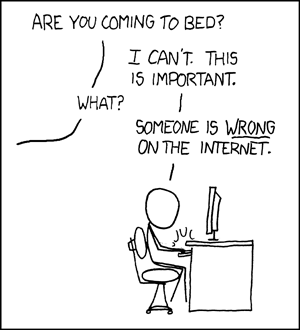
\includegraphics[width=3cm]{bilder/duty_calls.png}\\\vspace{5mm}
    }
}

Die Hochschulpolitik befasst sich mit allen politischen Vorgängen
bezüglich der Hochschulen in Deutschland. Dies beinhaltet Abläufe in den
Landes"= und Bundesparlamenten, den Gremien der universitären
Selbstverwaltung und der Öffentlichkeit. Thematisch umfasst die
Hochschulpolitik unter anderem den Bau, die Finanzierung, den rechtlichen
Status der Hochschulen, den Rahmen für Forschung und Lehre, aber auch die
soziale Stellung der Studierenden.

So wird über Studien"= und Prüfungsordnung, Organisation, Gliederung und
Ausrichtung der Hochschulen weitestgehend vor Ort entschieden, während
andere Entscheidungen die Kompetenz der Universität übersteigen. Sehr
deutlich wird dies bei den Regelungen über das BAföG
(Bundes"=Ausbildungsförderungs"=Gesetz), Wohnheimmieten oder kommunale
Verkehrspolitik (Fahrradwege, Semesterticket, \dots).

Die studentischen Belange werden bei der Entscheidungsfindung leider
häufig nur unzureichend berücksichtigt. Eine Ursache hierfür ist durch das
Hochschulrecht gegeben, welches den Studierenden nur eine bescheidene
Mitwirkung in den offiziellen Gremien der Universität zugesteht. Eine
Mitarbeit in anderen Gremien der Bildungslandschaft ist überhaupt nicht
vorgesehen. Natürlich gibt es Überschneidungen zwischen den Interessen der
Studierenden und denen des Landes bzw. des Bundes als Träger und
Finanziers der Hochschulen im Großen sowie zwischen den Studierenden und
den ProfessorInnen vor Ort. Die Entscheidungen, die in den letzten Jahren im
Bereich der Hochschule getroffen wurde, lassen allerdings deutlich
erkennen, dass diese Interessen im Vergleich zum Sparwillen der
öffentlichen Kassen nur geringe Priorität besaßen.

Ein weiterer Grund für die vergleichsweise geringe Beachtung der
Studierenden in Entscheidungsfindungsprozessen ist deren Situation und
sozialer Status. Zum einen sind die Studierenden keine homogene Gruppe:
Die einen finanzieren sich ihr Studium selbst, während andere durch ihre
Eltern unterstützt werden -- wieder andere werden von
einer Stiftung gefördert. Andererseits ist die Studienzeit gewöhnlich nur
ein auf politischer Skala kurzer Lebensabschnitt, der nach wenigen Jahren
wieder beendet ist. Die Wirkung von heute beschlossenen, politischen
Entscheidungen betrifft in den meisten Fällen erst die Studierenden von
morgen.

Umso wichtiger ist die studentische Mitwirkung aus eigenem Engagement. Der
folgende Artikel stellt den institutionellen Rahmen dar, in dem sich
politische Arbeit von Studierenden an der Universität und darüber hinaus
bewegt.

\subsection{Gesetzlicher Rahmen}
Grundsätzlich ist Hochschulrecht Landesrecht. Der Bund gab lange Zeit im
Hochschulrahmengesetz (HRG) Vorgaben, die im Landesrecht ausgestaltet
wurden. Am 26. Januar 2006 wurde vor dem Bundesverfassungsgericht (BVG)
ein Kompetenzstreit über die Zuständigkeit in der Hochschulpolitik
zwischen dem Bund und den Bundesländern Baden"=Württemberg, Bayern, dem
Saarland, Sachsen, Sachsen"=Anhalt und Hamburg geklärt. Der Bundestag hatte
in der 6. Novelle des Hochschulrahmengesetzes ein „in der Regel
gebührenfreies Erststudium“ verlangt und die Einführung von Verfassten
Studierendenschaften zwingend vorgeschrieben. (Die Verfassten
Studierendenschaften werden im Laufe dieses Artikels noch besprochen.) Das
Verfassungsgericht stellte fest, dass der Bund in diesen Fragen solange
nicht zuständig ist, bis die Notwendigkeit einer einheitlichen Regelung
für die Herstellung gleicher Lebensverhältnisse in den verschiedenen
Ländern nachgewiesen wurde. Die Fragestellung, ob eventuell einzuführende
Studiengebühren der Verfassung entsprechen, wurde dabei nicht verhandelt.
Seit der Förderalismusreform im Jahr 2006 ist die Gesetzgebungskompetenz
vollständig auf die Länder übergegangen. Der Bund ist lediglich indirekt
z.B. über das BAföG (Bundesausbildungsförderungsgesetz) oder
Forschungsförderungsprojekte (z.B. die Exzellenzinitiative) eingebunden.
Amtierende Ministerin auf Bundesebene ist \wissenschaftsministerbund.


Die Wissenschaftsministerin in Baden"=Württemberg ist zur Zeit \wissenschaftsministerbawue.
Das wesentliche Landesgesetz für die Form der
baden"=württembergischen Hochschulen wurde durch das seit 1. Januar 2000
geltende Universitätsgesetz (UG) bestimmt. Am 9. Dezember 2004
verabschiedete der Landtag von Baden"=Württemberg ein neues
Landeshochschulgesetz (LHG), das insbesondere Änderungen in der
Kompetenzverteilung zwischen den Gremien der universitären
Selbstverwaltung vorsah. Ziel schien dabei zu sein, Kompetenzen weg von
Gremien hin zu Einzelpersonen zu verlagern. So wurden dem Senat, dem
traditionellen akademischen Entscheidungsgremium der Universität (mit
Mitgliedern aller Gruppen und Fakultäten) zahlreiche Kompetenzen genommen
und auf das Rektorat übertragen. Genaueres zu den Gremien der Universität
und ihrer Verflechtung erfahrt ihr weiter unten. Die Möglichkeiten des
Wissenschaftsministeriums, auf die Besetzung der Position des Rektors und
die Zusammensetzung des Aufsichtsrates einzuwirken, wurden gesteigert.

Die aktuelle grün-rote Landesregierung hat eine Novelle des LHGs ausgearbeitet, 
die am 27.03.2014 als „Drittes Hochschulrechtsänderungsgesetz“ beschlossen wurde.
Inwiefern sich die dortigen Änderungen konkret auf den Alltag an den Universitäten 
auswirken werden, wir abzuwarten sein.


\subsection{Aus der jüngsten Geschichte der Mitbestimmung an den Hochschulen}
%\mathphyssecnobar{Aus der jüngsten Geschichte der Mitbestimmung an den Hochschulen}

\sidebar{
    \centering
    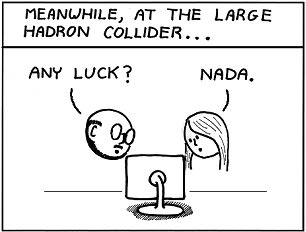
\includegraphics[width=3cm]{bilder/dear_CERN_1.png}\\\vspace{14mm}
    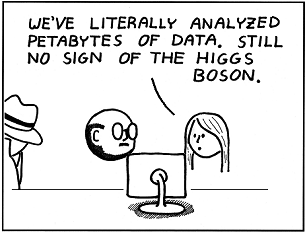
\includegraphics[width=3cm]{bilder/dear_CERN_2.png}\\\vspace{14mm}
    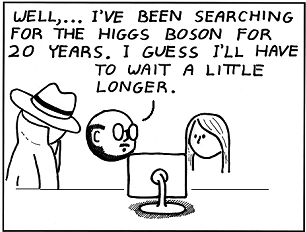
\includegraphics[width=3cm]{bilder/dear_CERN_3.png}\\\vspace{14mm}
    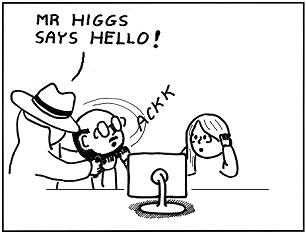
\includegraphics[width=3cm]{bilder/dear_CERN_4.png}\\\vspace{14mm}
    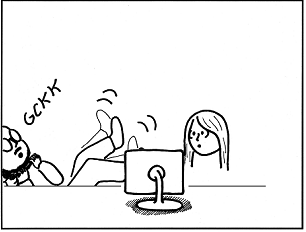
\includegraphics[width=3cm]{bilder/dear_CERN_5.png}\\\vspace{14mm}
    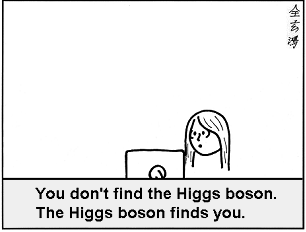
\includegraphics[width=3cm]{bilder/dear_CERN_6.png}
}

Bis 1969 hatten die LehrstuhlinhaberInnen (Ordinarien) das Sagen an den
Universitäten. Sie hatten praktisch die alleinige Entscheidungsbefugnis
für ihrenjeweiligen Lehr"= und Forschungsbereich. Sämtliche Gremien setzten
sich alleine aus LehrstuhlinhaberInnen zusammen. 1969 wurde diese
Ordinarienuniversität im Zuge der Forderungen nach Demokratisierung und
Mitbestimmung abgeschafft und die Gruppenuniversität eingeführt. Die
Mitglieder der Universität wurden in Gruppen eingeteilt, die
ProfessorInnen, die wissenschaftlichen MitarbeiterInnen (=\ Mittelbau), die
StudentInnen sowie die sonstigen MitarbeiterInnen (=\ Sonstige). Jeder
dieser „Stände“ wählt bei Uniwahlen eine bestimmte Anzahl VertreterInnen
in die Gremien der Uni. Der „erste Stand“, die ProfessorInnen, stellen
zusätzlich eine gewisse Anzahl von Mitgliedern kraft Amtes. Für eine kurze
Phase wählten alle Gruppen außer den Sonstigen (HausmeisterInnen,
SekretärInnen, \dots) gleich viele VertreterInnen („Drittelparität“).
1973 stellte das Bundesverfassungsgericht (mit 6:2 Stimmen) aber fest, dass
aufgrund der grundgesetzlich garantierten Freiheit von Forschung und Lehre
(Art. 5 GG) die Gruppe der ProfessorInnen in allen Gremien eine
maßgebende, bzw. in bestimmten Fragen eine ausschlaggebende Mehrheit haben
muss. Damit ist eine relative bzw. in einigen Gremien eine absolute
Mehrheit gemeint. Aufgrund dieses Urteils sind die Entscheidungsgremien so
zusammengesetzt, dass ProfessorInnen mindestens so viele Sitze haben wie
alle anderen Gruppen zusammen.



\section{Studentische Vertretung}
Um die Interessen der Studierenden artikulieren und durchsetzen zu können,
muss es eine Instanz geben, die sie vertritt. In einigen Bundesländern
(ab 01. Januar 2013 allen außer Bayern) nimmt diese Aufgabe die
Verfasste Studierendenschaft (VS) war, d.h. die Studierenden geben sich
in eine Vertretung, meistens einen Studierendenrat (StuRa)
oder auch ein Studierendenparlament, der/das eine „Regierung“, den AStA
(Allgemeiner Studierendenausschuß) wählt, welcher die Beschlüsse der VS
vollzieht und z.B. über die zur Verfügung stehenden Finanzen beschließt.
Die Rechte der Verfassten Studierendenschaft können dabei sogar so weit
reichen, dass diese als Gemeinschaft öffentlichen Rechtes eigene Verträge
abschließen kann -- oft basieren Semestertickets auf solchen Verträgen.

In Baden"=Württemberg gab es schon einemal (bis 1977) eine Verfasste
Studierendenschaft. Um die Studierenden vor politischen Dummheiten zu
bewahren, wurde jedoch 1977 - als weitere Folge des Urteils von 1973 - in
den Ländern Bayern und Baden"=Württemberg die VS in der bisherigen Form
vorsichtshalber abgeschafft. Da es aber einem demokratischen Staat mit
folglich demokratischen Universitäten wiedersprach, wenn die
zahlenmäßig stärkste Gruppe ausgeschaltet wird, richtete man einen
besonderen Ausschuss des Senats ein: den Ausschuss für musische,
sportliche, geistige und soziale Belange der Studierenden. Diesen rein
beratenden Ausschuss bezeichnete man einfach genauso wie die bisherige
Studierendenvertretung als AStA (im folgenden nur noch als sogenannter
AStA, „AStA“ bezeichnet). Er wird gebildet aus den studentischen
Mitgliedern des Senats und einigen KandidatInnen entsprechend der
erhaltenen Stimmenanzahl. Tätig werden durfte der baden"=württembergische
Pseudo-„AStA“ gemäß LHG nur unter der Rechtsaufsicht des Rektors. Zu
Fragen des Studiums, zu Problemen einzelner Fachbereiche oder gar zu
politischen Fragen, z.B. BAföG oder Semesterticket darf der „AStA“ nicht
aktiv werden. Eine Vertretung auf Fachbereichsebene war überhaupt nicht
vorgesehen.

Auf diese Beschneidung ihrer Rechte reagierten die
Studierenden, indem sie ihre eigenen Vertretungen parallel zur
Pseudovertretung im „AStA“ schufen. Im Gegensatz zu den abhängigen,
offiziellen Gremien wurden sie als unabhängige Gremien bezeichnet.
An vielen Fachbereichen gibt es kontinuierlich oder immer mal wieder
Institutsgruppen, Fachschaftsinitiativen oder unabhängige Fachschaften,
die sich durch öffentliche Treffen und ihre Arbeit am Fachbereich
(Gremienarbeit, Klausurensammlung, Vorlesungsumfragen, Feten,
ErstsemesterInneneinführungen) legitimieren. Sie setzen sich vor Ort für
die Belange der Studierenden eines Faches ein. Diese Vertretungs"= und
Arbeitsstrukturen ersetzten wirkungsvoll die bisher fehlende gesetzlich verankerte
Mitbestimmung oder gar Vertretung. Wie die Zusammenarbeit mit den
jeweiligen Instituten oder Seminaren klappt, hängt jedoch immer noch vom
Wohlwollen der ProfessorInnen, des Rektors/der Rektorin und des Ministeriums ab. In den
Fachbereichen Mathematik, Physik und Informatik übernahm diese Aufgabe
seit 1983 die Fachschaft MathPhys\footnote{\url{http://mathphys.fsk.uni-heidelberg.de}}.
Im Zuge der Einführung der Verfassten Studierendenschaft (siehe folgender Absatz) hat sich der Zusammenschluss MathPhys
wieder in die drei Teilfachschaften Mathematik, Informatik und Physik aufgeteilt.
Das gemeinsame „Dach“ MathPhys ist aber erhalten geblieben, um fachschaftsübergreifende
Arbeit zu koordinieren und weiterhin einen kollegialen Austausch zu ermöglichen.


\subsection{Ein Klassiker kehrt zurück: die VS}

Mit dem „Gesetz zur Einführung einer Verfassten Studierendenschaft und
zur Stärkung der akademischen Weiterbildung
(Verfasste-Studierendenschafts-Gesetz - VerfStudG)“ hat der Landtag am 27. Juni 2012
die Wiedereinführung\footnote{Offiziell ist nur von der „Einführung“ die
Rede, da die neue VS nicht die offizielle Rechtsnachfolge der alten VS sein soll.
Grund ist, dass das Land andernfalls höhere Millionenbeträge zurückzahlen müsste,
die der VS 1977 enteignet wurden.} der Verfassten Studierendenschaft beschlossen.

Über die Form der Verfassten Studierendenschaft -- also die Frage, welche
Struktur die studentische Selbstverwaltung bekommen sollte -- haben die Studierenden
der Universität Heidelberg vom 13. bis 15. Mai 2013 per Urabstimmung abgestimmt.
Es standen zwei Modelle zur Auswahl: Ein Modell mit zwei
Kammern (Studierendenparlament und FSK) sowie ein Modell mit nur einer
Kammer (ein sog. Studierendenrat). Unsere Fachschaft hatte nach intensiven Diskussionen mit
VertreterInnen beider Initiativen einen eindeutigen
Konsens dahingehend gefunden, dass sowohl für unsere Studierenden aus
Mathe/Info/Physik/Astronomie, als auch für die Studierendenschaft
insgesamt das Zweikammernmodell deutlich größere Vorteile besitzt als
das Einkammernmodell\footnote{Wen unsere Gründe interessieren, sie sind in unserem FS-Info-Heft MPI 1-2013 nachlesbar}.
Bei der Urabstimmung hat sich allerdings die Mehrheit der Studierenden (58,87\%)
für das Einkammernmodell ausgesprochen, weshalb wir im Folgenden nur dieses Modell beschreiben.



\subsection{Die Gremien der VS}

Die Verfasste Studierendenschaft gliedert sich in Heidelberg in sogenannte
Studienfachschaften. Eine Studienfachschaft umfasst alle
Studierenden eines Faches, in eurem Fall gehört ihr also zu einer der
Studienfachschaften Informatik, Mathematik oder Physik\footnote{Falls ihr
mehr als ein Hauptfach studiert -- z.B. im Lehramtsstudiengang -- werdet
ihr standardmäßig der Studienfachschaft eures ersten Hauptfaches zugeordnet.
Sofern ihr in eurem zweiten Hauptfach wählen möchtet, müsstet ihr dorthin „optieren“.
Details hierzu findet ihr auf der Homepage des Wahlamts der Universität}.
Bitte prüft in der Zeit vom 11. bis 18. Oktober euren Eintrag im Wäherverzeichnis
(einsehbar auf der Homepage des Wahlamts). Sofern ihr dort nicht auftaucht,
dürft ihr bei der Wahl vom 18. bis 20. November nicht wählen.

Auf Ebene der Studienfachschaften gibt es zwei Organe: Eine „Vollversammlung“ 
(auch „Fachschaftssitzung“ genannt) und einen gewählten „Fachschaftsrat“. In den 
Fachschaften Informatik, Mathematik und Physik haben wir uns dafür entschieden, 
den Fachschaftsrat als lediglich ausführendes Organ zu gestalten, die 
Entscheidungskompetenzen liegen bei der regelmäßig statt findenden Fachschaftssitzung.
Das bedeutet, ihr könnt ohne euch extra wählen lassen zu müssen jederzeit
auf Fachschaftsebene mitarbeiten und mitentscheiden.

Auf zentraler Ebene gibt es in Heidelberg als legislatives Orgen den Studierendenrat (StuRa). 
Er besteht aus VertreterInnen aller Studienfachschaften, die von diesen entsandt werden
(ca. 64 Personen) sowie aus direkt durch die Studierenden gewählten Mitgliedern.
Die Anzahl der direkt gewählten Mitglieder skaliert mit der Wahlbeteiligung
und liegt zwischen 0 Personen (bei 0\% Wahlbeteiligung) und ebenfalls 64 Personen
(bei 50\% oder höherer Wahlbeteiligung).

Der Studierendenrat beschließt als zentrales legislatives Organ über alle
zentralen Belange der Studierendenschaft (Höhe der Beiträge, Finanzen,
Wahl der Referate, etc.).

Das exekutive Organ der VS ist in Heidelberg die sogenannte „Referatekonferenz“ sein.
Sie besteht aus vom Studierendenrat für bestimmte Aufgabenbereiche (z.B.
Kommunales, Ökologie, Hochschulpolitik, Soziales, \dots) gewählten
ReferentInnen. Diese setzen Beschlüsse des StuRa um und können sogar --
sofern der StuRa keine Entscheidung treffen kann oder (z.B. weil zu
wenige Mitglieder anwesend sind) nicht beschlussfähig ist --
eigenständig im Namen der Studierendenschaft entscheiden.

\subsection{Hintergründe zur VS}

\paragraph{Mitgliedschaft in der Verfassten Studierendenschaft}

Alle Studierenden sind qua Immatrikulation automatisch Mitglied der
Verfassten Studierendenschaft. Weil sie die einzige Möglichkeit zur
Partizipation an legitimierter Studierendenvertretung ist und ihre
Leistungen für alle Studierenden offen stehen müssen, ist ein Austritt
nicht möglich.

\paragraph{Rechtsfähigkeit}

Bisher ist der „AStA“ (Allgemeiner Studierendenausschuss) nur ein Ausschuss
im Gesamtgebilde Universität. Durch die Verfasste Studierendenschaft wird
die Studierendenvertretung zu einer eigenständigen, rechtsfähigen Teilkörperschaft
innerhalb der Universität. Dadurch kann sie selbst Verträge abschließen und
so z.B. mit den Verkehrsbetrieben direkt über das Semesterticket verhandeln
oder Leasing-Fahrzeuge vergünstigt an die Studierenden vermieten.
Diese Rechtsfähigkeit gilt allerdings nur für die VS als ganzes,
nicht für ihre Organe (z.B. Fachschaften).

\paragraph{Beitragshoheit}

Die VS kann von allen Studierenden Beiträge erheben, die zusammen mit dem
sonstigen Semesterbeitrag eingezogen werden. Mit der Einführung der VS
wurde leider nicht festgeschrieben, dass das bisherige von der Uni verwaltete
Budget des „AStA“, auf das die Studierendenvertretung zurückgreift,
bestehen bleibt. Die VS erhebt deshalb einen Beitrag von \EUR{7.50} pro 
Semester. Von diesem werden qua Satzung 40 Prozent an die dezentrale 
Studierendenvertretung durch Fachschaften fließen, der Rest wird auf zentraler, 
sprich universitätsweiter Ebene durch den StuRa verwaltet Damit soll nicht 
nur die schon vor Einführung der VS verrichtete Arbeit fortgeführt, sondern 
auch die Etablierung und Förderung neuer studentischer Projekte, besserer 
Kampagnen zur Vertretung derstudentischen Interessen und mehr Service ermöglicht 
werden.

\paragraph{Mandat}

Früher war der offizielle „AStA“, also der Senatsausschuss mit 11 gewählten
Mitgliedern, mit einem sportlichen, kulturellen, musischen und eingeschränkt
sozialen Mandat ausgestattet.
Mit dem Gesetz erhält die neue VS zusätzlich zu den alten Kompetenzen ein
hochschulpolitisches und soziales Mandat; sie darf sich außerdem zum Wirken
der Hochschule in der Gesellschaft äußern, z.B. durch Technikfolgenabschätzung,
sowie die politische Bildung der Studierenden fördern. In diesem Sinne hat
sie ein politisches Mandat. Dabei ist sie an das übliche Neutralitätsgebot
für staatliche Organe mit Pflichtmitgliedschaft gebunden, darf also z.B.
keine Werbung für religiöse oder parteipolitische Strukturen machen.

\section{Entscheidungsgremien der Universität}
Die Universität Heidelberg ist eine Lehr"= und Forschungseinrichtung mit
über 500 ProfessorInnen, circa 31\,000 Studierenden und vielen sonstigen
MitarbeiterInnen. Der Etat der Universität beträgt um die 620 Millionen
Euro. Die Aufgabe der Universität, die „Pflege und Entwicklung der
Wissenschaften und der Künste durch Forschung, Lehre und Studium“ (§2
% Quelle: http://www.umwelt-online.de/recht/allgemei/laender/bw/hschg01.htm
LHG), stellt hohe finanzielle und organisatorische Ansprüche.
Entscheidungen für die gesamte Hochschule treffen die zentralen Gremien,
Rektorat, Senat und Universitätsrat. Der Senat beschließt über
universitätsweite Belange wie Verlegung der Semesterzeiten, die
Immatrikulationsordnung und generell über grundlegende Fragen, welche die
Gesamtuniversität betreffen. Der Senat bestätigt Vorschläge der einzelnen
Fachbereiche über die Berufung neuer Professoren, genehmigt Lehrpläne und
beschließt über die Einrichtung oder Aufhebung von Studiengängen. Dem
Senat gehören außer dem Rektorat alle DekanInnen (das sind die
Vorsitzenden der Fakultäten), die Frauenbeauftragte und 8 gewählte
ProfessorInnen, 4 Studierende, 4 VertreterInnen aus dem Mittelbau und 4
Sonstige an. Das macht also ein Verhältnis von 27, bzw. 28 Profs gegen 12
andere, davon 4 Studis. Besondere Themen wie Umweltfragen oder
Prüfungsangelegenheiten werden in beratenden Ausschüssen des Senats
vorbereitet, in denen alle Gruppen vertreten sind, die ProfessorInnen
natürlich mit absoluter Mehrheit.

\sidebar{
    \centering
    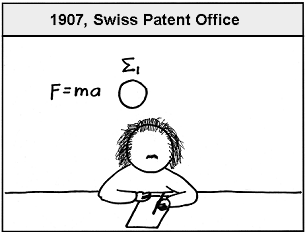
\includegraphics[width=3cm]{bilder/inequivalence_principle_1.png}\\\vspace{13mm}
    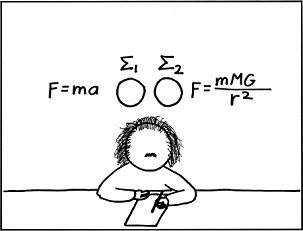
\includegraphics[width=3cm]{bilder/inequivalence_principle_2.png}\\\vspace{13mm}
    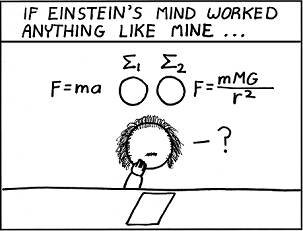
\includegraphics[width=3cm]{bilder/inequivalence_principle_3.png}\\\vspace{13mm}
    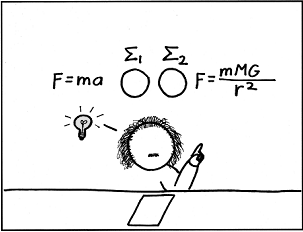
\includegraphics[width=3cm]{bilder/inequivalence_principle_4.png}\\\vspace{13mm}
    \includegraphics[width=3cm]{bilder/inequivalence_principle_5.png}\\\vspace{13mm}
    \includegraphics[width=3cm]{bilder/inequivalence_principle_6.png}
}


Den Universitätsrat gibt es erst seit dem Wintersemester 2000/2001. Er ist
eine Art Aufsichtsrat der Universität. Er berät über die strukturelle
Ausrichtung der Universität und hat das letzte Wort in
Finanzangelegenheiten. Er besitzt damit wesentlichen Einfluss auf die
künftige Entwicklung der Universität. 6 der 11 Mitglieder sind
Universitätsexterne aus Politik, Kultur und Wirtschaft, 5 Mitglieder
kommen aus der Universität. Alle Mitglieder werden vom
Wissenschaftsministerium benannt. Im Zuge der Novelle des LHG 2014 wurde
der Universitätsrat mit weiteren Kompetenzen ausgestattet.

Sieht man den Universitätsrat als Aufsichtsrat der Universität, wird das
Rektorat zum zugehörigen Vorstand. Es besteht aus dem/der RektorIn, 4
ProrektorInnen und dem/der LeiterIn der Verwaltung: dem/der KanzlerIn.
Rektor ist zur Zeit \rektor . Neben seinen Verwaltungsaufgaben in
der Uni, vertritt er sie auch nach außen, z.B. gegenüber dem Land. Das
Rektorat residiert in der alten Universität, Grabengasse 1. Die
Universitätsverwaltung ist in der Seminarstr. 2 angesiedelt.

\subsection{Die Fakultät}

Die speziellen Fragen eines Fachbereichs werden in der Fakultät, der
„organisatorischen Grundeinheit der Universität“, die „gleiche oder
verwandte Fachbereiche zusammenfasst“ (LHG), (vor)entschieden. Die
Universität Heidelberg ist in zwölf Fakultäten gegliedert, zum Beispiel 
die Fakultät für Mathematik und Informatik und die Fakultät für Physik und 
Astronomie. Während man an einigen Fakultäten nur ein bzw. wenige Fächer studieren
kann, gibt es andere Fakultäten, wie z.B. die Neuphilologische Fakultät,
an denen viele Fächer (Germanistik, Anglistik, Romanistik etc.) studiert
werden können. Geleitet wird die Fakultät von einem/einer DekanIn und dem
ihm unterstehenden Dekanat, das die laufenden Geschäfte erledigt. Der/Die
DekanIn wird für vier Jahre vom Fakultätsrat gewählt. Zur Zeit ist Dekan der
Mathematik Prof. \dekanmathe{} und in der Physik Prof. \dekanphysik. Zusammen mit dem
Studiendekan (s.u.) bilden Dekan und Prodekan den Fakultätsvorstand. Zu
finden ist das Dekanat der Mathe \gls{INF} 288, Zimmer 277 und das der Physik
INF 226, 2.OG.

Die Mitglieder der Fakultäten wählen in dem beschriebenen
Vierklassenwahlrecht den Fakultätsrat, das oberste Gremium der Fakultät.
Er ist zuständig für alle Fragen der Lehre und der Forschung. Ihm gehören
6 gewählte Profs, 5 Studierende, 4 Angehörige aus dem Mittelbau und 1 Mitglied
aus der Gruppe der MitarbeiterInnen aus Administration und Technik
an, außerdem alle InstitutsdirektorInnen und der Fakultätsvorstand, also Dekan,
Prodekan und Studiendekan. Abweichend davon kann sich eine Fakultät auch für einen
sogenannten „großen Fakultätsrat“ entscheiden (so geschehen beispielsweise in der 
Fakultät für Physik und Astronomie), in dem alle ProfessorInnen der Fakultät 
Mitglied sind. Die Mitgliederanzahlen der anderen Gruppen werden dabei ebenfalls
(leicht) erhöht. Der Fakultätsrat bildet Ausschüsse mit vergleichbarer
Zusammensetzung, die sich um bestimmte Bereiche kümmern, besonders wichtig
sind zum Beispiel die Prüfungsausschüsse oder die Studienkommissionen. Die
Mitglieder der Ausschüsse müssen nicht immer Mitglieder des Fakultätsrats
sein. Die Fakultäten gliedern sich weiter in Institute. Jedes Institut
wird von einem Institutsdirektor geleitet.

\subsection{StudiendekanIn und Studienkommission}

Mit dem Universtätsgesetz von 1995 wurde ein weiteres Gremium auf Fakultätsebene 
eingeführt: die Studienkommission. Diese ist ein Gremium, das den Studiendekan/die
StudiendekanIn, der/die Kraft Amtes ihr Vorsitzender/ihre Vorsitzende ist, berät.
StudiendekanIn und Studienkommission sollen gemeinsam zur Verbesserung der Lehre
beitragen. Die Studienkommission besteht aus StudiendekanIn, drei weiteren
ProfessorInnen, zwei VertreterInnen des Mittelbaus sowie vier Studierenden.
Hauptaufgaben der Kommission sind:
\begin{itemize}
    \addtolength{\itemsep}{-0.7\baselineskip}
    \item Empfehlungen zur Weiterentwicklung von Gegenständen und Formen des Studiums
    \item „Verfahren zur Bewertung und Verbesserung  der Qualität der Lehre unter
          Einbeziehung studentischer Veranstaltungskritik“ zu entwickeln
    \item In regelmäßigen Abständen einen Lehrbericht zu verfassen.
\end{itemize}

Die Umsetzung von Empfehlungen und die Wahrnehmung laufender Aufgaben
obliegt dem Studiendekan/der Studiendekanin. Die Kommission ist nur
beratend und die Durchsetzung ihrer Beschlüsse und Ideen ist vom guten
Willen des Fakultätsrats abhängig. Der Studiendekan / die Studiendekanin
nimmt die mit Forschung und Lehre zusammenhängenden laufenden Aufgaben
wahr; seine/ihre Aufgabe ist es insbesondere, auf ein ordnungsgemäßes und
vollständiges Lehrangebot hinzuwirken und die Beschlussfassung über
Studienpläne, Studien"= und Prüfungsordnungen und Lehrberichte
vorzubereiten.



% !TEX ROOT = ../ersti.tex
%
% TODO: stefanzen

%\section{Studiengebühren ade!}
\newpage
\mathphyssecnobar{Studiengebühren ade!}%FIXME
Seit dem Sommersemester 2012 sind die Studiengebühren, die im Sommersemester 2007 in ganz BaWü in Höhe von \EUR{500} eingeführt wurden, wieder abgeschafft. Es erfolgte ein vollständiger finanzieller Ausgleich in Höhe von \EUR{280} aus Landesmitteln, genannt "Qualitätssicherungsmittel", oder liebevoll: "QuaSiMi". Es sind nur \EUR{280} statt \EUR{500}, weil durch Ausnahmeregelungen wie die legendäre "Geschwisterregelung" seit 2009 im Durchschnitt nur dieser Betrag pro eingeschriebener Person an Studiengebühren eingenommen wurde.

Die QuaSiMi sind nicht nur zusätzliche Landesmittel für die Hochschule, sondern auch weiterhin zweckgebunden für die Verbesserung der Studienbedingungen. Außerdem wurde im Gesetz \footnote{StuGebAbschG vom 21.12.2011 \url{http://mwk.baden-wuerttemberg.de/fileadmin/pdf/gesetze/StuGebAbschG/GBl-2011_565_Studiengeb\%C3\%BChrenabschaffungsgesetz_21122011.pdf}} festgeschrieben, dass die QuaSiMi nur im Einvernehmen mit einer legitimierten Vertretung der Studierenden ausgegeben werden dürfen. Das heißt, keine Ausgabe kann gegen den Willen der Studis durchgesetzt werden. Das ist immerhin ein Schritt in Richtung Fairness und Gleichberechtigung.

\subsection*{Gebührenfreiheit?}
Weiterhin müsst ihr jedoch als Teil der \EUR{\beitragssumme}, die ihr jedes Semester an die Uni überweisen müsst, einen "Verwaltungskostenbeitrag" von \EUR{\verwaltungsbetrag} bezahlen. Dieser wird den Hochschulen auf ihren Etat angerechnet, sodass das Geld de facto als Ersparnis ans Land Baden-Württemberg geht. Weil das Land nach der nächsten Wahl die Studiengebühren als Mittel gegen die erste Anhebung des Hochschuletats seit 1996 wiederentdecken könnte, möchten wir das Thema Studiengebühren nicht einfach als Teil der hochschulpolitischen Geschichte abhaken, sondern in diesem Kapitel daran erinnern.
%Dieser Absatz sollte dann rein, wenn unten der historische Exkurs nicht hineinkommt!
\iffalse
Wir laden Euch darüberhinaus ein, Euch über die Hintergründe der Studiengebühren zu informieren, beispielsweise auf unserer Fachschaftshomepage \footnote{http://mathphys.fsk.uni-heidelberg.de/studgeb-historie.html}.
\fi
%

\subsection*{Ein paar Argumente gegen Studiengebühren}

Wie ihr sicher bemerkt habt, gehen wir davon aus, dass es gut sei, wenn es keine Studiengebühren gibt. Was veranlasst uns dazu, mal abgesehen von persönlicher Betroffenheit?
\begin{itemize}
\item {Barrieren zwischen Abi und Studium einreißen!}\\Ein Studium ist verglichen mit einer Ausbildung sehr teuer. Mit Studiengebühren wäre es nochmals knapp \EUR{100}/Monat teurer. Das schreckt nachweislich insbesondere AbiturientInnen ab, deren Eltern selbst nicht studiert haben. Außerdem schreckt es prozentual mehr Mädchen als Jungs ab. Kurzum: Menschen, deren Umgebung von ihnen traditionell weniger erwartet dass sie studieren, studieren weniger; gesellschaftliche Ungleichheit, Stratifizierung und überkommene Rollenbilder werden fortgeschrieben.
\item {Aufhebung von finanziell bedingten Nachteilen im Studium!}\\Studis, die knapp über die BAföG-Grenze fallen, sind am härtesten von Studiengebühren betroffen. Denn bei ihnen reicht das Geld der Eltern oft nicht, um Lebensunterhalt und Gebühren zu finanzieren. Sie müssen also jobben gehen und haben somit deutlich weniger Zeit, sich um ihr eigentliches Studium zu kümmern. Gerade in Zeiten der Master"=Zulassungsbeschränkung führt das im Endeffekt zu finanzieller Auslese.
\item {Bildung ist öffentliches Gut!}\\Die Einführung der Studiengebühren wurde von eingefrorenen Haushälten und massiven Kürzungen im Bildungsbereich seitens der Landesregierungen flankiert. Studiengebühren sind keine Notwendigkeit der Lage, sondern Politik. Unserer Auffassung nach ist Bildung jedoch eins der wichtigsten Güter einer Gesellschaft, und das meinen wir nicht im rein ökonomischen Sinn. Gerade die universitäre Bildung bietet (noch, vergleichsweise) viele Freiräume zum eigenständigen Denken. Dessen Bedeutung ist für eine Gesellschaft, die sich demokratisch nennen möchte, nicht zu unterschätzen. Deshalb sollte Bildung in den Landeshaushalten höchste Priorität haben.
\end{itemize}
%\vfill
%\begin{figure}[h]
%\centering{
%    \includegraphics[width=0.7\textwidth]{bilder/studiengebuehren.png}
%}
%\end{figure}
%\vfill

\subsection*{Verteilung der QuaSiMi an der Universität Heidelberg}

Die Studierenden in Heidelberg setzten durch, dass die Studiengebühren ausschließlich zur Verbesserung der Lehre verwendet werden durften. Um ausreichend Präsenz in den Diskussionen zu haben, wurde auch durchgesetzt dass Studierende in den Kommissionen zur Verteilung der Gelder die absolute Mehrheit haben. Die studentischen VertreterInnen der Kommission werden auf Vorschlag der Fachschaft vom Fakultätsrat gewählt. Diese Gremien haben allerdings nur beratende Funktion. Der von der Kommission beschlossene Verwendungsplan wird dem Fakultätsrat zur Entscheidung vorgelegt. Die Budgetverantwortung liegt beim Dekanat.

Diese Struktur wurde bei Einführung der QuaSiMi oftmals übernommen. An einigen Fakultäten, darunter die für Physik \& Astronomie, wurde die Kompetenz der Mittelverwendung an die Studienkommission übergeben und die Studiengebührenkommission aufgelöst.

\subsection*{Verwendung der QuaSiMi}

Der größte Teil des Gelds, etwa 80\%, geht an Deine Fakultät. Das Rektorat verfügt über 20\% der Mittel als zentrale QuaSiMi, wobei vor jeder Ausgabe das Einvernehmen mit den Studierenden in der zentralen QuaSiMi-Kommission hergestellt werden muss. Daraus geht auch Geld an die zentralen Einrichtungen der Universität, also an die Bibliothek, das Rechenzentrum oder den Hochschulsport. Aktuell werden viele Anträge diverser Einrichtungen und Institute an die zentrale QuaSiMi-Kommission entschieden.

Die einzelnen Fächer haben in den letzten Semestern die ihnen zur Verfügung stehenden Gelder nur teilweise ausgegeben, sodass insgesamt noch eine Summe von
%  STIMMT DIE SUMME??
\EUR{1,3\,Mio} auf den einzelnen Konten der Fakultäten liegen. Deshalb versucht das Rektorat immer wieder durchzusetzen, dass mehr Gelder in zentrale Einrichtungen fließen. Allerdings regt sich hier seitens der Fakultäten und der studentischen Vertretung Widerstand.
%Unklar ist auch, wie viel Prozent das Rektorat einbehalten wird.

Die größten Defizite im Bereich Lehre waren an unseren Fakultäten das schlechte Betreuungsverhältnis, vor allem in den Übungsgruppen und Seminaren, sowie ein ungenügendes Serviceangebot. Um diese Defizite auszugleichen wurde und wird mit den Sondermitteln aus Studiengebühren und QuaSiMi insbesondere in folgende Bereiche investiert:

\vspace{5mm}
\textbf{Mathematik und Informatik}
\begin{itemize}
 \item {Mitarbeiterstellen}\\Lehr-/Servicepersonal, Lehraufträge, AssistentInnen
\item {Hilfskraftmittel}\\ TutorInnen und zusätzliche Übungsgruppen
\item {Ausstattung}\\ Computerpools, Hörsäle, Seminarräume
\item {Materialien}\\ Softwarelizenzen, Skripte, Bücher, eBooks\footnote{\url{http://www.ub.uni-heidelberg.de/helios/epubl/eb/Welcome.html}}, Zeitschriften
\end{itemize}

Weiter wurden Mittel zur Modernisierung der mangelhaften Ausstattung der Hörsäle,
Computerpools, sowie der Bibliothek investiert.

\vspace{5mm}
\textbf{Physik}
\begin{itemize}
\item {Mittelbaustellen}\\Medizinerausbildung, Studienberatung, Lehramtsausbildung, Aufbau des IUP (Glossar) Praktikums
\item {AP + FP Versuche (Glossar)}\\Modernisierung bestehender Versuche, neue
Praktika im FP und dem IUP
\item {Öffnungszeiten}\\Erweiterung der Öffnungszeiten in der \gls{KIP}-Bibliothek sowie dem Studierendensekretariat
\item {Hilfskraftmittel}\\ TutorInnen und zusätzliche Übungsgruppen
\item {Materialien}\\Skripte, Bücher, eBooks\footnote{\url{http://www.ub.uni-heidelberg.de/helios/epubl/eb/Welcome.html}}, Zeitschriften
\end{itemize}

Da experimentelle Erfahrung enorm wichtig für einen Physiker ist, wurde und wird
viel Geld in aktuellste Versuche investiert. Eine Bereicherung stellen sicher auch
die Exkursionen nach vielen Kursvorlesungen dar (CERN, GSI\dots).

%VON 2008...
%Eine genauere aktuelle Auflistung findet ihr im aktuellen MathPhys-Info
%(siehe FS-Homepage\footnote{\url{http://mathphys.fsk.uni-heidelberg.de/mpi.html}}).

%Wenn das Erstiinfo zu fett wird, kann man das rausnehmen      ––– wird gemacht ;)
\iffalse
\subsection*{Historischer Exkurs: Geschichte der Studiengebühren -- Geschichte der Sparprogramme}

Im Wintersemester 1970/71 wurden in der Bundesrepublik Deutschland die allgemeinen Studiengebühren, damals "Hörergeld", mit Hilfe von Protesten und Boykotten abgeschafft.

Aber immer wieder gab es Bewegungen in der Politik, die Studiengebühren forderten. Das ging meistens mit einem Bild von Universität einher, das diese nicht als öffentliche Einrichtung zur Verbreitung des gesellschaftlichen Guts Bildung, sondern als Anbieterin von Leistungen auf dem Markt der Ware Bildung auffasst. Entsprechend wenig ist solche Politik bereit, Bildungseinrichtungen eine angemessene finanzielle Ausstattung zukommen zu lassen.

Es wurden Rückmeldegebühren eingeführt um die Haushaltslöcher der Hochschulen zu stopfen. Die Hochschulen mussten in BaWü Anfang der 1990er arge Kürzungen im Haushalt hinnehmen, der 1996 für 10 Jahre eingefroren wurde (bis auf Baumaßnahmen). Diese geplante finanzielle Austrocknung der Hochschulen wurde übrigens 2006 um weitere 10 Jahre verlängert. Gleichzeitig wurde damals laut darüber nachgedacht, Studiengebühren für Langzeitstudierende einzuführen. Diese wurden in verschiedenen Ländern auch durchgesetzt (in BaWü zum WS 1998/99).

2002 wurde von der Kultusministerkonferenz ein allgemeines Studiengebührenverbot festgeschrieben. Langzeitstudiengebühren waren in bestimmten Ausnahmefällen erlaubt.

Gegen dieses Verbot klagten einige Bundesländer vorm Bundesverfassungsgericht, darunter BaWü. Sie führten an, dass der Bund seine Gesetzgebungskompetenz überschritten und in die Länderkompetenz eingegriffen habe.

Am 26.01.2005 fällte das Bundesverfassungsgericht das Urteil, dass ein Verbot allgemeiner Studiengebühren nur gerechtfertigt sei, um „gleichwertige Lebensbedingungen“ in den Ländern zu wahren. In diesem Fall sei aber kein Anlass zu solcher Sorge gegeben. Somit wurde das Gesetz von 2002 gekippt und der Weg für die allgemeinen Studiengebühren geebnet.

Schon im Dezember 2005 wurde in Baden"=Württemberg Minister Frankenbergs Gesetzentwurf zur Einführung allgemeiner Studiengebühren von der Landesregierung beschlossen. Studiengebühren in Höhe von \EUR{500} pro Semester wurden zum Sommersemester 2007 eingeführt. Es gab weiter Proteste gegen die Einführung, Demos und Boykotts wurden organisiert.

Der AK Studiengebühren der \gls{FSK} organisierte einen Boykott und es wurden Klagen beim Verwaltungsgericht eingereicht. Wie an vielen anderen Universitäten in Baden"=Württemberg wurden die Studierenden in Heidelberg von der studentischen Vollversammlung dazu aufgefordert, die \EUR{500} nicht an die Universität, sondern auf ein Treuhandkonto zu überweisen. Man hätte dann unter Bezug auf das zurückgehaltene Geld als Druckmittel mit der Landesregierung Gespräche begonnen. Leider wurde das beschlossene Quorum mit nur ca. 1200 statt 4500 eingegangenen Zahlungen nicht erreicht und der Boykott daher nicht durchgeführt. Die Studiengebühren konnten damit nicht abgeschafft werden.

Auch im Bildungsstreik, der 2009-2011 die Bildungspolitik aufrüttelte, war die Forderung nach Abschaffung der Studiengebühren (als einer Bildungsgebühr von vielen) stets zentral. Darum organisierten viele baden"=württembergische Bildungsstreik-Gruppen, auch in Heidelberg, nach den Erfahrungen aus Hessen und NRW im Hinblick auf die Landtagswahl nochmals Demonstrationen im Januar 2011. Von SPD über Grüne bis Linkspartei fand sich im Wahlprogramm zur Landtagswahl 2011 denn auch die Absichtserklärung wieder, die Studiengebühren abzuschaffen.

Zum Sommersemester 2012 hat nun tatsächlich die grün-rote Landesregierung ihr Wahlversprechen eingelöst: Die Studiengebühren wurden, bei voller Kompensation aus Landesmitteln, abgeschafft!

%Von Gebühren befreit bist du auch schon in diesem Semester, wenn du ein Kind unter 14 Jahren hast, ein Praxissemester absolvierst, ein Stipendium erhältst, du mindestens zwei (auch Stief"=/Halb"=) Geschwister hast die nicht diese baden"=württembergische Geschwisterregelung in Anspruch nehmen, oder du unter einer studienerschwerenden Behinderung leidest. Eine Befreiung aufgrund außerordentlicher Studienleistungen ist gesetzlich möglich, wird aber von den Fakultäten für Mathematik und Physik abgelehnt und darum nicht gewährt.
\fi

% !TEX ROOT = ../ersti.tex
% 
% TODO stefanzen
% 
% Nicht vergessen die Copyright Zeile im Impressum wieder einzufügen
% —done!

%\section{Semesterticket}
\mathphyssecnobar{Semesterticket}
Seit mehr als 15 Jahren hat Heidelberg ein Semesterticket, 
das es den Studierenden ermöglicht kostengünstig den öffentlichen
Nahverkehr zu nutzen.
Zur Einführung waren alle Beteiligten von der großen Resonanz überrascht
und das Ticket entwickelte sich zu einem Erfolg.
Enorme Preissteigerungen von 127\% in den vergangenen 10\,Jahren haben
jedoch dazu geführt, dass die Nutzerzahlen deutlich sinken und 
das Semesterticket von vielen als unattraktiv und überteuert wahrgenommen 
wird.

Ein Semesterticket muss stets eine Vielzahl von Interessen befriedigen. Es 
sollte ein attraktives und günstiges Ticket im Stadtbereich sein und das 
direkte Umfeld des Hochschulstandortes erschließen. Des Weiteren ist es wünschenswert die ländliche Region anzubinden und den dort wohnhaften Studierenden einen Umzug und hohe Mieten zu ersparen. Neben dem täglichen Pendelverkehr ist die Heimreise zum elterlichen Wohnsitz ebenfalls für eine Vielzahl von Studierenden ein Grund ein Semesterticket zu erwerben.

Das aktuelle Semesterticket in Heidelberg wird vom Verkehrsverbund Rhein-Neckar (VRN) angeboten und gilt für ein Semester. Es berechtigt zu Fahrten im gesamten Tarifgebiet\footnote{\url{http://www.vrn.de/linienplaene/netzlinienplaene/gesamtnetz/}} -- „einem Schlauch von Polen nach Frankreich“\footnote{Zitat aus der Semesterticket Umfrage der FSK}. Die Ausdehnung ist in Ost-West Richtung sehr weitreichend, in Nord-Süd Richtung ist jedoch nach 20\,km von Heidelberg aus Schluss. Das Semesterticket finanziert sich aus einem Kaufpreis von aktuell \EUR{150} und einem solidarischen Sockelbeitrag von \EUR{25.80}, den alle Studierenden mit dem Studentenwerksbeitrag bei der Rückmeldung zahlen müssen -- auch wenn sie das Ticket nicht nutzen. Eine Heidelberger Besonderheit bei der Sockelfinanzierung ist, dass sie es allen Studierenden ermöglicht ab 19 Uhr innerhalb der Großwabe Heidelberg sowie den Waben Dossenheim, Eppelheim und Leimen kostenlos mit Bus und Bahn fahren zu können -- der Studiausweis gilt dabei als Fahrschein.


\subsection{Konflikt ums Semesterticket}
\marginpar{
    \centering
    \vspace{1mm}
    \includegraphics[width=3cm]{bilder/straba.pdf}
}
Seit Herbst 2008 verhandeln das Verkehrsreferat der Studierendenvertretung und das Studentenwerk mit dem VRN über einen neuen Vertrag. Die Studis fordern ein Ende der enormen Preissteigerungen, um auch in Zukunft mit dem Semesterticket ein günstiges Nahverkehrsangebot zu gewährleisten. Da der VRN jedoch weiter an Preissteigerungen von ca. 10\% pro Jahr festhalten will, stand das Semesterticket vor dem Aus. 
Nach einem Übergangsvertrag, auf den der VRN sich im WS 09/10 in letzer Minute eingelassen hat, wurde im WS 13/14 erneut verhandelt. Diesmal kam der Kommunalwahlkampf in Heidelberg den Studis zu Gute, aber trotz massiven Drucks aus der Politik und Zuschüssen durch den Gemeinderat ist das Semesterticket nach wie vor recht teuer und der VRN wird die Preise weiterhin regelmäßig erhöhen.

Eine Neuerung bei den letzten Vertragsverhandlungen war, dass der frisch eingerichtete \gls{StuRa} alle Studis zu einer Urabstimmung über das Vertragsangebot aufgerufen hat. Auch wenn die Urabstimmung wegen teils schwerer Formfehler von verschiedenen Seiten angefochten wurde, hat sich doch eine Mehrheit der Abstimmenden für das Semesterticket ausgesprochen, sodass der StuRa dem Vertragsangebot letztendlich zugestimmt hat.\\[1em]

Heidelberg ist eine eher kleine übersichtliche Stadt in welcher alles bequem mit dem Fahrrad erledigt werden können -- meist sogar schneller als mit Bus und Bahn. Dank der milden Temperaturen ist dies auch im Winter durchaus möglich. Wenn ihr in Heidelberg selbst wohnt ist daher gut zu überlegen ob sich ein Semesterticket lohnt oder man wie viele Andere das Fahrrad nutzt.

Weitere Informationen zu den Verhandlungen und dem Semesterticket findest du unter: \url{http://www.stura.uni-heidelberg.de/semesterticket}

%~ \begin{figure}[h]
%~ \centering{
    %~ \includegraphics[width=\textwidth]{bilder/purity.png}
%~ }
%~ \end{figure}




%%%%%%%%%%%%%%%%%%%%%%%%%%%%%%%%%%%%%%%%%%%%%%%%%%%%%%%%%%%%%%%%%%%%%%%%%%%%%
\chapter{Die Fachschaft MathPhys}
\label{diefsmathphys}
% !TEX ROOT = ../ersti.tex
\section{Die Fachschaft MathPhys}
Wir, die „Fachschaft“, sind ein Haufen von Studis quer durch alle Semester und auch immerhin zwei Fakultäten (Physik \& Astro sowie Mathe \& Info), die sich als basisdemokratisch organisierte, unabhängige Vertreterin der Physik"=, Mathe"= und Informatik"=Studis sieht. Folglich sind alle Studis der beiden Fakultäten in der Fachschaft willkommen, redeberechtigt und stimmberechtigt. Genaueres zur Arbeitsweise der Fachschaft findest du auf den nächsten Seiten.

Im weiteren Sinne sind die „Fachschaft“ alle Studierenden der Mathe, Physik oder Informatik. Ihr seid mit eurer Immatrikulation Teil der „Fachschaft“, wenn auch nicht unbedingt aktiv beteiligt. Ihr habt das Recht, Entscheidungen zu fällen – nutzt es!

Seit Einführung der Verfassten Studierendenschaft zum Wintersemester 2013/2014 befindet sich die Fachschaft allerdings in einem Umstrukturierungsprozess, da die Verfasste Studierendenschaft die bisherige Struktur nicht unterstützt. Bisher besteht die Umstrukturierung hauptsächlich aus der Aufspaltung der vormals gemeinsamen Sitzung in drei verschiedene Sitzungen, die der Dreh\= und Angelpunkt unsere Arbeit sind.

\begin{center}
\large
\textbf{Fachschaftssitzungen}

\textbf{jeden Mittwoch um 18 Uhr \gls{c.t.}}
\end{center}

\sidebar{
  \centering
  \chaptersidebarpushdown
  \ifthenelse{\boolean{druckversion}}{
        \includegraphics[width=3cm]{fs-logo_bw.pdf}
    }{
        \includegraphics[width=3cm]{fs-logo_4c.pdf}
    }
}

\subsection*{Alles verändert sich, wenn ihr es verändert\dots}
Wie bereits erwähnt, sehen wir unsere Aufgabe in der Studierendenvertretung. Dabei kommt es uns insbesondere darauf an, dass wir die von uns vertretenen Studiengänge verbessern. Darüber hinaus mischen wir uns manchmal auch in politische Fragestellungen an der Uni ein. Das alles geschieht auf vielerlei Weise.

Wenn ihr dieses Heft in den Händen hälst, habt ihr sicher schon von unserer Erstieinführung gehört oder daran teilgenommen. Sie soll den Schock der ersten Uniwoche abmildern und ist in der Regel der erste Berührungspunkt mit uns für eineN Ersti an der Uni Heidelberg.

Zu Beginn des Semesters werdet ihr in einigen Veranstaltungen Skripte ausgeteilt bekommen. Diese drucken wir, wenn die Profs ein Skript bereitstellen, für die laufenden Veranstaltungen seit dem Sommersemester 2008 aus Studiengebühren"=/Qualitätssicherungsmitteln. Wenn ihr die Skriptausgabe verpasst, kommt einfach in den Fachschaftsraum und fragt nach ob es noch welche gibt.

Während des Semesters arbeiten wir aktiv in den Gremien und Kommissionen der Fakultäten, wo wir die studentischen Interessen so gut vertreten, wie es die Umstände erlauben.
In den Studienkommissionen wird über Prüfungsordnungen, Zulassungsordnungen und generell alles was die Lehre an der Fakultät als ganzes betrifft, diskutiert. Auch über die Verwendung der Qualitätssicherungsmittel, welche die Studiengebührenmittel ersetzen, wird in der Studienkommission beraten. Hier wird ausgearbeitet, wie das Studium ablaufen soll -- entsprechend wichtig ist es, dass wir uns dazu in den Fachschaftssitzungen eine Meinung bilden und diese in den Kommissionen vertreten.
In den Berufungskommissionen, wo über die Berufung neuer ProfessorInnen an die Uni Heidelberg entschieden wird, setzen wir uns dafür ein, dass gute DidaktikerInnen mit spannendem Lehrangebot berufen werden.
Nach der Vorarbeit durch die Kommissionen diskutieren und entscheiden die Fakultätsräte als fakultätsweite Gremien. Die 5 bzw. 6 studentischen VertreterInnen in den Fakultätsräten der Mathe \& Info bzw. Physik \& Astro werden jährlich von allen Studis gewählt und kommen aus der Fachschaft.
Darüberhinaus erarbeiten und diskutieren wir universitätsweite Finanzierungs"= und Positionierungsanträge aus der Fachschaftskonferenz (FSK).
%!!!WICHTIG. die FSK gibt es nicht mehr, was machen wir da?!
Spätestens wenn sich das Semester zum Ende neigt, werdet ihr einen Service unsererseits zu schätzen wissen: Den Verleih von Altklausuren oder Prüfungsberichten für die Zwischenprüfungen. Auch wenn die Umstellung auf Bachelor und Master bereits einige Semester zurück liegt und wir für viele Fächer Altklausuren und Berichte haben, freuen wir uns immer über neuen Input. Insbesondere bei nicht obligatorischen Veranstaltungen und im Master ist der Vorrat noch mager. Von daher der Appell an euch: Bringt eure Klausuren ins Fachschaftsbüro und schreibt fleißig Prüfungsberichte, denn ihr habt ja schließlich auch davon profitiert.


\subsection*{Ich will lieber tanzen gehn\dots}
Um mit den hartnäckigen Vorurteilen gegenüber der Zunft der PhysikerInnen, InformatikerInnen und MathematikerInnen aufzuräumen (und natürlich um selbst Spaß zu haben) veranstalten wir einmal im Semester das legendäre MathPhysTheo-Fest und  mehrere Spieleabende.
Lange Zeit verstalteten wir zusammen mit der Fachschaft Romanistik das legendäre Fest „MathPhysRom“. Seit 2011 erbeten wir göttlichen Beistand und feiern nun zusammen mit der Fachschaft Theologie. Auch wenn das „MathPhysTheo“ nun einen neuen Namen trägt, ist es immernoch legendär, also: Kommt, tanzt, feiert und \dots Helft mit! Wir suchen immer HelferInnen in allen möglichen Bereichen. Als Dankeschön bekommt ihr ein tolles T-Shirt, Getränke- und Garderobengutscheine und natürlich freien Eintritt! Keine Sorge, ihr habt trotz Helferschicht noch genug Zeit um euren Uni-Zettel-Frust rauszutanzen.

Wenn das dann nicht reichen sollte, gibt es immer noch unseren Fachschaftsraum INF 305, Raum 045, als Anlaufstelle.
Am Philweg gibts außerdem die Caféte. Dies ist ein altes Gartenhäuschen im Philosophenweg 12, das wir im Sommer 2009 liebevoll renoviert und 2013 wieder nutzbar gemacht haben. Neben Sofas und Tischchen stehen auch Kaffeemaschine, Wasserkocher und Tassen drin. Kaffee und Tee gibt es zum Selbstkostenpreis und ab und zu stehen auch Kekse oder Gummibärchen da.

Falls euch das noch nicht genug Informationen sind, ihr etwas nicht verstanden habt, oder ihr Interesse an Mitarbeit habt, dann schaut einfach vorbei und fragt. Noch besser ist es allerdings, wenn ihr in der Fachschaftssitzung vorbeischaut. Dort laufen sozusagen alle Fäden zusammen, es wird diskutiert und beschlossen.

Einmal im Semester fahren wir auf das \gls{FSWE} irgendwo hin, meist tief in den Odenwald. Das Wochenende dient dazu alle fachschaftsrelevanten Themen ausführlich in einzelnen AKs (Arbeitskreise) besprechen zu können und natürlich nicht zuletzt um einander besser kennen zu lernen und Spaß zu haben. Für Erstis ist die Teilnahme kostenlos und von der Verpflegung könnte sich die Mensa mehr als nur eine Scheibe abschneiden.

% !TEX ROOT = ../ersti.tex
\section[Studierendenvertretung in der Fachschaft]{Studierendenvertretung in der Fachschaft -- Wer vertritt meine Interessen?}

Verkürzt heißt die Antwort: Vertritt Dich selbst!

Das Wort „Studierendenvertretung“ als Beschreibung für die Arbeit der Fachschaft MathPhys ist ein wenig missverständlich, weil man meinen könnte, dass einmal im Jahr eine Vertretung der Studierenden gewählt wird, die dann schon die Arbeit macht. Offiziell ist das auch so, weil das Landeshochschulgesetz es so vorschreibt. Tatsächlich meint „Studierendenvertretung“ hier jedoch die Vertretung der Studierenden durch sie selbst -- uns alle.

\subsection*{Offenheit der Fachschaft}

Deshalb passiert die meiste Arbeit in den Fachschaftssitzungen und in Arbeitskreisen. In einer Sitzung sind alle Studenten des jeweiligen Fachs willkommen, redeberechtigt und können an jedem Entscheidungsprozess gleichberechtigt mitwirken.

Offiziell werden die Fachschaft zwar auch vertretungsdemokratisch durch die jährliche Wahl von Fachschaftsmitgliedern in den Fakultätsrat legitimiert. Allerdings ist seit ewigen Zeiten zu dieser Wahl keine andere Liste als die Fachschaftsliste angetreten\dots denn tatsächlich zieht die Fachschaft ihre Legitimation aus ihrer basisdemokratischen Offenheit. Statt nur einmal im Jahr zur Urne zu trotten, kannst Du jede Woche bei der Fachschaftssitzung selbst mitentscheiden!

\subsection*{Mandatierung der GremienvertreterInnen}

Wer als VertreterIn der Fachschaft in Gremien gewählt wird, ist nicht nur dem eigenen Gewissen verpflichtet, sondern der ganzen Fachschaft. Diese diskutiert alle Themen, die im Gremium wahrscheinlich relevant werden, findet eine Fachschaftsposition, und beauftragt die Gewählten, diese Position zu vertreten. Die GremienvertreterInnen werden somit von der Fachschaftssitzung meistens imperativ mandatiert.

%\newpage

\subsection*{Arbeitskreise und Arbeitsgruppen der Fachschaft}

In zwei großen Fakultäten mit Studis vom ersten Semester bis zur Doktorarbeit gibt es natürlich äußerst verschiedene Interessen, und jedeR setzt eigene Prioritäten. Das ist super, weil daraus total verschiedene Aktivitäten entstehen -- vom Spieleabend bis zur Vortragsreihe über IT-Sicherheit finden diverse Ideen im Fachschaftsumfeld engagierte MitstreiterInnen für ihre Umsetzung.

Damit nicht die ganze Fachschaftssitzung darüber diskutieren muss, ob man neben Brettspielen auch Rollenspiele anbietet, gibt es verschiedene Arbeitskreise (AKs) der Fachschaft, die bei Bedarf in den Sitzungen berichten. Wenn eine Entscheidung oder Geld benötigt wird, entscheidet die Sitzung. Dort werden auch AK-Gründungen bekanntgegeben.

\subsection*{Entscheidungsfindung in der Fachschaft: Die Vielfalt der Interessen aushandeln}

%\sidebar{\parbox{3.5cm}{%Infobox Konsensstufen
\vspace*{-2em}

\subsubsection*{Konsensstufen}
\footnotesize
Wenn die Konsensstufen in einer Fachschaftssitzung abgefragt werden, kannst du durch die Zahl ausgestreckter Finger an deiner Hand anzeigen, wie Du zu einem Vorschlag stehst.
\begin{description}
\item[1. Vorbehaltlose Zustimmung]
Ich finds gut so.
\item[2. Zustimmung trotz leichter Bedenken]
Ich habe ein wenig Sorge, aber halte den Vorschlag grundsätzlich für eine gute Idee.
\item[3. Enthaltung]
Ich möchte nicht an der Entscheidung mitwirken, aber trage deren Ergebnis mit.
\item[4. Beiseitestehen]
Ihr könnt das für euch so entscheiden, aber ich mach da nicht mit.
\item[5. Schwere Bedenken]
Kein Konsens! Ich finde den Vorschlag echt scheiße.
\item[Faust = VETO]
Kein Konsens! Dieser Vorschlag widerspricht meinen Prinzipien. Entweder wird er unterlassen, oder wir müssen ab jetzt getrennte Wege gehen, möglicherweise sogar gegeneinander arbeiten.
\end{description}
}} %das passt leider nicht

Die verschiedenen Interessen und Prioritäten der Studis sind aber auch eine Herausforderung. Die Fachschaft lebt davon, dass die verschiedensten Studis ihre Gedanken und ihre Position einbringen und vertreten. Es gibt also a priori keine „Fachschaftsmeinung“, es gibt nur die Fülle der Einzelmeinungen, die durch alle Anwesenden wieder verändert wird. Die verschiedensten Ansichten zu einer gemeinsamen Position und Handlungsweise zusammenzubringen, ist dann die anspruchsvolle Aufgabe der Fachschaftssitzung.

Methodisch verwenden wir dabei ein Konsensstufensystem. Das heißt, zuerst werden alle angehört, die etwas zur Diskussion beizutragen haben. Angesichts dessen werden Vorschläge gemacht, wie man in der Frage vorgehen könnte. Deren Vor- und Nachteile werden abgewogen. Schließlich macht jemand einen Vorschlag für das Vorgehen der Fachschaft, den diese Person als konsensfähig einschätzt. Zu diesem werden die Konsensstufen (vgl. Infobox!) unter den Anwesenden abgefragt.

Alle, die keine vorbehaltlose Zustimmung angezeigt haben, können sich dann dazu äußern, warum sie nicht einfach zustimmen. Leichte Bedenken bis größere Vorbehalte (Konsensstufe 2"=4) können so bei der Umsetzung des Vorschlags bedacht und berücksichtigt werden. Vielleicht ergibt sich daraus auch ein noch besserer Vorschlag.

Wenn kein Konsens erreicht wurde (Konsensstufe 5 oder Veto), wird die Diskussion unter Berücksichtigung der Beweggründe fortgeführt, um auszuloten, ob nicht doch ein konsensfähiger Vorschlag möglich ist. Wenn das nicht der Fall ist, muss die Entscheidung entweder unterlassen werden, oder man geht ab da getrennter Wege. Letzteres ist noch nicht geschehen, seit wir im Mai 2012 das Konsensstufensystem eingeführt haben.
Bisher ist immer eine für alle tragfähige Lösung gefunden worden. Wir sehen das als große Stärke des Konsensprinzips. Es schließt aus, dass jemand übergangen wird. Wie man vorgeht, wenn die Ansichten doch einmal unvereinbar sind, müsste besprochen werden, wenn es passiert. Wichtig ist hier nur, dass die Möglichkeit besteht, getrennter Wege zu gehen, wenn man feststellt, dass man politisch gegeneinander arbeiten möchte.

%\vfill
\vspace*{\parskip}\null

\noindent\framebox{\parbox{\textwidth}{%Infobox Konsensstufen
\vspace*{-2em}

\subsubsection*{Konsensstufen}
\footnotesize
Wenn die Konsensstufen in einer Fachschaftssitzung abgefragt werden, kannst du durch die Zahl ausgestreckter Finger an deiner Hand anzeigen, wie Du zu einem Vorschlag stehst.
\begin{description}
\item[1. Vorbehaltlose Zustimmung]
Ich finds gut so.
\item[2. Zustimmung trotz leichter Bedenken]
Ich habe ein wenig Sorge, aber halte den Vorschlag grundsätzlich für eine gute Idee.
\item[3. Enthaltung]
Ich möchte nicht an der Entscheidung mitwirken, aber trage deren Ergebnis mit.
\item[4. Beiseitestehen]
Ihr könnt das für euch so entscheiden, aber ich mach da nicht mit.
\item[5. Schwere Bedenken]
Kein Konsens! Ich finde den Vorschlag echt scheiße.
\item[Faust = VETO]
Kein Konsens! Dieser Vorschlag widerspricht meinen Prinzipien. Entweder wird er unterlassen, oder wir müssen ab jetzt getrennte Wege gehen, möglicherweise sogar gegeneinander arbeiten.
\end{description}
}}

\subsection*{Die schöne Theorie und die reale Umsetzung}

Dir wird bestimmt einiges an der hier vorgestellten Arbeitsweise komisch vorkommen, vielleicht hast Du auch Einwände. Wir laden Dich zunächst ein, es Dir einfach mal anzuschauen! Wenn dann noch Diskussionsbedarf und Kritik an der Arbeitsweise besteht, kann und soll dies unbedingt angesprochen werden. Nichts von dem, was hier beschrieben wurde, ist in Stein gemeißelt; unsere Arbeitsweise wird ständig an unsere Erfordernisse angepasst.

Wir sind uns dessen bewusst, dass partizipative Demokratie zeitlich viel Einsatz verlangt. Solange wir die Studiengänge nicht so umgestaltet kriegen, dass allen genug Zeit dafür bleibt, ist das auch ein Legitimationsproblem. Durch Transparenz über aktuelle Themen und Entscheidungen schaffen wir Abmilderung. Doch bisher bleibt unsere Öffentlichkeitsarbeit hinter unserem Anspruch zurück. Da Fachschaftsarbeit freiwillig und ehrenamtlich ist, wird eben genau das gemacht, wofür sich jemand (ggf. mit ein bisschen Erwartungsdruck\dots) freiwillig Zeit nimmt. Wenn Du Lust darauf hast, bist Du herzlich dazu eingeladen, die Öffentlichkeitsarbeit zu verbessern! Wir freuen uns, und es gibt immer Leute, von denen man hier einiges lernen kann.

Natürlich sind Basisdemokratie und Konsensprinzip auf dem Papier leichter, als in der Realität. Man ist daran gewöhnt, dass Konflikte nicht durch Aushandlung eines Konsens gelöst, sondern durch Abstimmung entschieden werden. Das heißt, man hat wenig Übung darin, Kompromisse zu finden, und viel Übung darin, die eigene Meinung ohne Abstriche durchzusetzen, was Gift für die Konsensfindung ist. Doch wir haben bisher die Erfahrung gemacht, dass das Konsensprinzip, obwohl es zunächst unproduktiver wirkt, wesentlich bessere Ergebnisse hervorbringt, und dadurch mit ein bisschen Übung effizienter ist als der Abstimmungsmodus.

Vielleicht mag es auf Dich so wirken, als seien alle in den Sitzungen ein eingeschworener Haufen, die eigentlich eh die gleichen Meinungen vertreten. Aber genau das versuchen wir zu verhindern, der Konsens wird von jeder Person gebildet, die ihre Meinung äußert. Egal in welche Richtung Deine Meinung geht, Du kannst sicher sein, dass sie zu einer Diskussion und einer neuen Meinungsbildung führt. Die Fachschaft sind alle, die sich einbringen wollen, mit all ihrer Persönlichkeit.

Dominanz mancher Leute in der Sitzung ist und bleibt ein Problem. Informationsgefälle versuchen wir durch kurze Inputs um 18 Uhr \gls{s.t.} vor der Sitzung abzubauen. Nachfragen ist erlaubt und erwünscht! Damit nicht einzelne die ganze Diskussion bestimmen, führen wir bei Bedarf Redelisten, wobei Leute vorgezogen werden, die erst wenig gesagt haben. Wenn Du Unbehagen mit Redeverhalten oder Diskussionsweise empfindest, teile das der Sitzung mit! Generell appellieren wir an unsere Reife. =)

Wir alle sind Lernende in fairem demokratischem Verhalten.

\subsection*{Feedback zu Arbeitsweise \& Diskussionskultur}

Da Du als Ersti einen recht unverklärten Blick auf die Fachschaftssitzung hast, sollst Du Gelegenheit bekommen, Deine Eindrücke zu äußern. Damit wir Kritik, Anregungen und Streitfragen zur Arbeitsweise der Fachschaft in Ruhe gemeinsam besprechen können, soll nach ein paar Sitzungen die Diskussion darüber in der Fachschaftssitzung geführt werden. Den Bedarf dafür kannst Du einfach in einer Sitzung anmelden, dann machen wir einen Termin dafür fest.


Haben wir Dein Interesse geweckt? Gut, dann sehen wir uns am Mittwochabend um 18:00 Uhr!

\begin{center}
\large
\textbf{Fachschaftssitzungen}

\textbf{jeden Mittwoch um 18 Uhr \gls{c.t.}}
\end{center}

\section{Das Vorkurs Team}
Die Vorkurse für Erstsemester werden von einer kleinen Gruppe an Leuten, die in
der Fachschaft MathPhys tätig sind, ehrenamtlich organisiert. Diese kümmern
sich um die Planung und Koordination der Fachvorträge und des Rahmenprogramms,
damit es zu einem reibungslosen Ablauf kommt.

Die Fachvorträge des Vorkurses Mathematik\footnote{die Vorträge im
Physikvorkurs werden seit geraumer Zeit von der Fakultät  verantwortet} werden
vollständig von StudentInnen der Fachschaft und des „Sympi-Sumpf“\footnote{Gruppe von Alt - Fachschaftlern, Freunden und allen die der FS
nahestehen} ausgearbeitet und gehalten. Darüber hinaus sind viele Studierned
der Info, Mathe und Physik als Helfer an der Durchführung der Spieleabende,
Kneipentouren und Wanderungen beteiligt. Dieses Engagement erfolgt ehrenamtlich
und unabhängig von den beiden Fakultäten. Alles in Allem sind mehr als 60
Personen in die Durchführung und Planung des Vorkurs involviert.

Der vor dem Vorkurs stattfindende Programmiervorkurs wird von zwei Studenten
verantwortet, die sich auch um das Skript für diesen kümmern.

Wenn du Lust hast, dich im nächsten Jahr beim Vorkurs zu engagieren, komm doch
einfach bei einer der FS - Sitzungen vorbei -- Helfer werden immer gebraucht
und sind herzlich willkommen. Auch im nächsten Jahr gilt es aufs Neue Spiele zu
planen, Referenten zu suchen, Räume zu reservieren und mit den Fakultäten zu
koordinieren.

\section{Das MathPhysTheo-Fest}

Das MathPhysTheo-Fest ist \emph{die} größte, komplett von Studis organisierte Party -- laute Musik, viel zu
trinken, jede Menge Leute (nicht nur Mathematiker, Informatiker und Physiker) -- ein \emph{Muss} für
alle feierwütigen Studierenden.  Es wird von den Fachschaften MathPhys und
Theologie gemeinsam veranstaltet und findet einmal pro Semester statt. Das Fest findet am \mathphystheotermin\ statt. Um euch von den Strapazen auf der Tanzfläche zu erholen, könnt ihr neben Bier zu günstigen Preisen auch leckere Cocktails trinken und euch mit Chili oder belegten Baguettes stärken.

Doch wer mal da war -- und das sind wie gesagt jede Menge Studis -- kann sich denken, dass da auch
jede Menge Organisation dahinter steckt. Damit beschäftigt sich der AK Fest. Wir
suchen dafür dringend Leute, die mitmachen! Wie der Ablauf funktioniert, ist
inzwischen schon gut getestet, aber trotzdem ist jedes Fest eine neue
Herausforderung. Um zu erfahren, wann sich der AK Fest trifft, könnt ihr Euch auf
die Mailingliste setzen. Das geht im Internet\footnote{\url{http://mathphys.fsk.uni-heidelberg.de/mailman/listinfo/akfest}} oder per E-Mail an \email{akfest@mathphys.fsk.uni-heidelberg.de}

Aber nicht nur für die Organisation, sondern auch für die vielen
Helferschichten, also Ausschank an der Theke, Auf- und Abbau
usw. suchen wir immer nach Helfern, also nach \emph{Dir}! Dafür hängen zu
gegebener Zeit Listen vor dem FS-Raum aus.




%%% Local Variables:
%%% mode: latex
%%% TeX-master: "ersti.tex"
%%% End:

%\input{fest}
%\section{Lehrevaluation}
\newpage\mathphyssecnobar{Lehrevaluation}
\label{eval}
\marginpar{
    \centering{
%        \vspace{20mm}
        \includegraphics{bilder/eval_1.png}\\
        \includegraphics{bilder/eval_2.png}\\
        \includegraphics{bilder/eval_3.png}\\
        \includegraphics{bilder/eval_4.png}\\
        \includegraphics{bilder/eval_5.png}\\
    }
}

\noindent Neben dem \hyperref[kummerkasten]{Kummerkasten} hast Du gegen Ende des
Semesters mit der \emph{Evaluation} noch eine Möglichkeit, Deine Profs und
TutorInnen zu bewerten. Das läuft dabei so ab, dass jemand von der Fachschaft
(in der Physik) oder von der ZUV (in der Mathe) in die Vorlesung kommt, eine
kleine Einleitung gibt und dann einen Bogen austeilt, den Du dann ausfüllst. In
den Tutorien der Mathe übernehmen die Tutoren die Evaluation.  Das ganze dient
zweierlei Zwecken: Zum Einen werden besonders schlechte (oder gute) Vorlesungen
mit den Dozierenden nachbesprochen um das Lehrniveau zu steigern bzw. zu
halten. Zum Anderen können Dir die Ergebnisse auch helfen, die richtigen
Vorlesungen oder Übungsgruppen zu wählen. Wenn der/die DozentIn sein/ihr
Einverständniss zur Veröffentlichung gegeben hat, dann findest Du die
Ergebnisse der letzten Semester z.B. vor dem Fachschaftsraum (im
Infoständer links der Tür), sowie im \gls{KIP}, im Hörsaalgebäude der Physik
(\Gls{INF} 308) und am Philosophenweg, jeweils an Infobrettern.

%\newpage\Large\mathphyssubsubsec{Volleyballturnier}\normalfont\small\\ \quad \\
%\section{Volleyballturnier}

% das Bild ist absichtlich in den Text eingebaut, weil die marginpar
% sonst verwirrt ist wegen des Seitenumbruchs (aka: it's complicated)
Einmal
\marginpar{
    \centering{
        \vspace{1mm}
        \includegraphics[width=3cm]{bilder/volley_nerdgag.png}\\
    }
}
im Semester beweisen wir, dass PhysikerInnen und MathematikerInnen sportlicher sind als ihr Ruf! Dazu wird zu studierendenfreundlichen Zeiten (ab 22 Uhr) im Olympiastützpunkt Volleyball gespielt und um Ruhm und Ehre gekämpft.
Seid also auch in diesem Semester dabei. Näheres zu Terminen und Anmeldung könnt ihr den zahlreichen Plakaten entnehmen oder einfach im FS-Raum nachfragen.

Der nächste Termin ist \volley.

\iftrue
\vfill

\begin{figure}[h]
    \centering
    \includegraphics[width=7cm]{bilder/volley_ballmond.jpg}
\end{figure}

\vfill
\fi


%%%%%%%%%%%%%%%%%%%%%%%%%%%%%%%%%%%%%%%%%%%%%%%%%%%%%%%%%%%%%%%%%%%%%%%%%%%%%
\chapter{Kontakte und Ansprechpartner}
% !TEX ROOT = ersti.tex
\section{Ansprechpartner im Studium}

Nicht nur am Anfang eures Studiums, sondern auch mitten drin, können kleinere und
größere Fragen und Probleme auftreten. Damit ihr mit diesen Problemen nicht alleine
da steht, gibt es mehrere Personen, die euch bei diesen helfen können. Erster
Ansprechpartner in allen Dingen ist natürlich die Fachschaft (siehe dazu Artikel
über die Fachschaft). Falls wir euch dann nicht weiter helfen können, gibt es an
jeder Fakultät noch weitere Ansprechpartner.

\newcommand{\proffoto}[2]{
    \centering
    \includegraphics[width=3cm]{#1}\\
    #2
    \vspace{4mm}
}

\begin{description}
\sidebar{
    \chaptersidebarpushdown
    \ifdefined\dekanphysikfoto
    \proffoto{\dekanphysikfoto}{\dekanphysiklang\\[-1ex]{\scriptsize Dekan Physik}}
    \fi

    \ifdefined\dekanmathefoto
    \proffoto{\dekanmathefoto}{\dekanmathelang\\[-1ex]{\scriptsize Dekan Mathe}}
    \fi

    \ifdefined\studiendekaninformatikfoto
    \proffoto{\studiendekaninformatikfoto}{\studiendekaninformatik\\[-1ex]{\scriptsize Studiendekanin Info}}
    \fi

    \ifdefined\studiendekanphysikfoto
    \proffoto{\studiendekanphysikfoto}{\studiendekanphysik\\[-1ex]{\scriptsize Studiendekan Physik}}
    \fi

    \vspace*{1.8cm}

    \ifdefined\studiendekanmathefoto
    \proffoto{\studiendekanmathefoto}{\studiendekanmathe\\[-1ex]{\scriptsize Studiendekan Mathe}}
    \fi

    \ifdefined\prodekanphyikfoto
    \proffoto{\prodekanphyikfoto}{\prodekanphysik\\[-1ex]{\scriptsize Prodekan Physik}}
    \fi

    % Rest weiter unten weil die Physik zwei Prodekane hat
    % und damit nicht mehr alles in die Spalten passt
}

\item[Der Dekan] ist sozusagen ChefIn der Fakultät und leitet diese. Er wird
	für vier Jahre gewählt. In der Mathe \& Informatik ist \dekanmathelang\
	Dekan, in der Physik \dekanphysiklang .

\item[Der Prodekan] ist VertreterIn des Dekans und unterstützt diesen in seinen
	Aufgaben. In der Mathe \& Informatik ist \prodekanmathe\ Prodekan, in der
	Physik \prodekanphysik .

\item[Das Dekanat] ist das Sekretariat der Fakultät. Hier kann euch geholfen
	werden, wenn ihr nicht wisst, an wen ihr euch genau wenden sollt. (In der
	Mathe: Tel.  \dekanatmathetelefon , in der Physik: Tel.
	\dekanatphysiktelefon )

\item[Der Studiendekan] ist Vorsitzender der Studienkommission. Diese ist für
	alle Fragen der Lehre zuständig und auch die erste Adresse bei Fragen und
	Problemen. In der Mathe ist \studiendekanmathe\ Studiendekan, in der
	Informatik \studiendekaninformatik , in der Physik \studiendekanphysik .

\item[Die Studienberatung] Fragen zur persönlichen Studienplanung, zur
	Orientierung und zur allgemeinen Beratung beantworten in jeder Fakultät
	eigens abgestellte Studienberater. So zum Beispiel \studienberatungmathe\
	in der Mathe, \studienberatunginformatik\ in der Informatik und
	\studienberatungphysik\ in der Physik.

\item[Deine Fachschaft] vertritt die Interessen der Studierenden in den
	Fakultätsgremien und ist diskreter Ansprechpartner bei Problemen mit einem
	Dozenten oder Fragen zur Prüfungsordnung. \\\fsraum;
	\url{fachschaft@mathphys.fsk.uni-heidelberg.de}

\item[Das Prüfungssekretariat] ist zuständig für Prüfungsfragen aller Art. Ob
	es jetzt um die Anrechnung von Modulen anderer Fakultäten, die Anmeldung
	von Bachelor-Arbeiten oder sonstige Fragen rund um die Prüfungsordnung
	geht, im Prüfungssekretariat sitzen kompetente Menschen, die dir
	weiterhelfen. In der Informatik ist das \pruefsekinfo, in der Mathe
	\pruefsekmathe, in der Physik \pruefsekphysik.

\item[BAföG-Beauftragter] Spätestens zu Beginn des 5. Semesters braucht ihr
	einen Leistungsnachweis, dass ihr die bei geordnetem Verlauf der Ausbildung
	bis zum Ende des 4. Fachsemesters üblichen Leistungen erbracht habt. Dies
	bestätigt Euch in der Mathe \bafogmathe , in der Informatik
	\bafoginformatik\ und in der Physik \bafogphysik .

\item[Lehramt] Alle Fragen, die das Lehramt betreffen, können euch im Zentrum
	für Lehrerbildung beantwortet werden: ZLB, Akademiestr. 3 Zimmer 237

\item[Gleichstellungskommissionen] setzen sich für die Chancengleichheit von
	Frauen und Männern ein und informieren über gesetzliche Regelungen. Falls
	ihr Fragen zum Thema Gleichstellung habt, könnt ihr euch jederzeit an sie
	wenden. Gleichstellungsbeauftragte in der Physik ist
	\frauenbeauftragtephysik\ (\url{gleichstellung@lsw.uni-heidelberg.de}), in
	der Mathe \& Informatik \frauenbeauftragtemathe .


\end{description}


\noindent Die Zuständigen für die jeweiligen Bereiche wechseln gelegentlich, können aber immer
aktuell auf den Internetseiten der entsprechenden Fakultäten eingesehen werden. Dort
findet ihr auch alle Sprechzeiten und Telefonnummern. Achtung: manchmal ist auch
eine vorherige Anmeldung erforderlich! Oft kann man die DozentInnen aber auch
außerhalb ihrer Sprechzeiten erreichen, zur Not immer per E-Mail.\\[.9cm]

\relax

% Hinweis zu den Abständen:
% die 1.3cm oben sind von Hand abgemessen, sodass der Abstand zwischen
% den Fotos in der Sidebar hier fortgesetzt wird
% die -5.52cm sind von Hand abgemessen, sodass die Fotos links bündig
% sind (bzw. die -1.695cm rechtsbündig für ungerade Seiten)
% die 1.51\textwidth sind auch von Hand abgemessen, sodass das Foto
% bzw. die Fotounterschrift (je nach dem was länger ist) rechts mit dem
% Text oben drüber bündig wird
% Alle Fotos sind 4 cm breit. Die Fotos in sollten alle das gleiche
% Seitenverhältnis (BxH: 200x267 bzw. wer Lust hat darf das kürzen)
% haben, wenn man unschöne Effekte vermeiden will
\iftrue
\checkoddpage
\ifoddpage
    %\hspace*{-1.695cm}
    \hspace*{-1.15cm}
\else
    \hspace*{-5.52cm}
\fi
\begin{minipage}{1.51\textwidth}
\parbox [t]{0.3\textwidth}{
    \ifdefined\prodekanmathefoto
    \proffoto{\prodekanmathefoto}{\prodekanmathe\\[-1ex]{\scriptsize Prodekan Mathe}}
    \fi
}
\hfill
\parbox[t]{0.3\textwidth}{
    \ifdefined\prodekanphysikfotoA
    \proffoto{\prodekanphysikfotoA}{\prodekanphysikA\\[-1ex]{\scriptsize Prodekan Physik}}
    \fi
}
\hfill
\parbox [t]{0.3\textwidth}{
    \ifdefined\prodekanphysikfotoB
    \proffoto{\prodekanphysikfotoB}{\prodekanphysikB\\[-1ex]{\scriptsize Prodekan Physik}}
    \fi
}
\end{minipage}
\else
\checkoddpage
\ifoddpage
    \hspace*{-1.695cm}
    %\hspace*{-1.15cm}
\else
    %\hspace*{-5.52cm}
    \hspace*{-4.55cm}
\fi
\begin{minipage}{1.51\textwidth}
%\hfill
\parbox [t]{0.24\textwidth}{
    \ifdefined\prodekanmathefoto
    \proffoto{\prodekanmathefoto}{\prodekanmathe\\[-1ex]{\scriptsize Prodekan Mathe}}
    \fi
}
\hfill
\parbox[t]{0.24\textwidth}{
    \ifdefined\prodekanphysikfotoA
    \proffoto{\prodekanphysikfotoA}{\prodekanphysikA\\[-1ex]{\scriptsize Prodekan Physik}}
    \fi
}
\hfill
\parbox [t]{0.24\textwidth}{
    \ifdefined\prodekanphysikfotoB
    \proffoto{\prodekanphysikfotoB}{\prodekanphysikB\\[-1ex]{\scriptsize Prodekan Physik}}
    \fi
}
\hfill
\parbox [t]{0.24\textwidth}{
    \ifdefined\studiendekanmathefoto
    \proffoto{\studiendekanmathefoto}{\studiendekanmathe\\[-1ex]{\scriptsize Studiendekan Mathe}}
    \fi
}
\end{minipage}
\fi

% Wenn noch Platz ist, z.B. weil Fotos fehlen oder die Physik
% nur noch einen Prodekan hat, kann man das als Lückenfüller nehmen:

%~ \begin{figure}[h]
%~ \vspace{10mm}
%~ \centering{
    %~ \includegraphics[width=\textwidth]{bilder/Prof.png}
%~ }
%~ \end{figure}




%%
\stepcounter{chapter}
\printglossaries

\end{document}
